% ******************************* PhD Thesis Template **************************
% Please have a look at the README.md file for info on how to use the template

\documentclass[a4paper,12pt,times,authoryear,index]{common/PhDThesisPSnPDF}

%\usepackage{draftwatermark}
%\SetWatermarkLightness{0.95}

% ******************************************************************************
% ****************************** Custom Margin *********************************

% Add `custommargin' in the document class options to use this section
% Set {innerside margin / outerside margin / topmargin / bottom margin}  and
% other page dimensions

\ifsetMargin
\else
    \RequirePackage[left=37mm,right=30mm,top=35mm,bottom=30mm]{geometry}
    \setFancyHdr % To apply fancy header after geometry package is loaded
\fi


%\chead{Unfinished draft}
%\cfoot{\texttt{Unfinished draft - compiled on \today{} at \currenttime}}

% *****************************************************************************
% ******************* Fonts (like different typewriter fonts etc.)*************

% Add `customfont' in the document class option to use this section

\ifsetFont
\else
    % Set your custom font here and use `customfont' in options. Leave empty to
    % load computer modern font (default LaTeX font).  

    \RequirePackage{libertine} 
\fi

% *****************************************************************************
% *************************** Bibliography  and References ********************

%\usepackage{cleveref} %Referencing without need to explicitly state fig /table

% Add `custombib' in the document class option to use this section
\ifsetBib % True, Bibliography option is chosen in class options
\else % If custom bibliography style chosen then load bibstyle here

   \RequirePackage[square, sort, numbers, authoryear]{natbib} % CustomBib

% If you would like to use biblatex for your reference management, as opposed to the default `natbibpackage` pass the option `custombib` in the document class. Comment out the previous line to make sure you don't load the natbib package. Uncomment the following lines and specify the location of references.bib file

% \RequirePackage[backend=biber, style=numeric-comp, citestyle=numeric, sorting=nty, natbib=true]{biblatex}
% \bibliography{References/references} %Location of references.bib only for biblatex

\fi


% changes the default name `Bibliography` -> `References'
\renewcommand{\bibname}{References}


% *****************************************************************************
% *************** Changing the Visual Style of Chapter Headings ***************
% Uncomment the section below. Requires titlesec package.

%\RequirePackage{titlesec}
%\newcommand{\PreContentTitleFormat}{\titleformat{\chapter}[display]{\scshape\Large}
%{\Large\filleft{\chaptertitlename} \Huge\thechapter}
%{1ex}{}
%[\vspace{1ex}\titlerule]}
%\newcommand{\ContentTitleFormat}{\titleformat{\chapter}[display]{\scshape\huge}
%{\Large\filleft{\chaptertitlename} \Huge\thechapter}{1ex}
%{\titlerule\vspace{1ex}\filright}
%[\vspace{1ex}\titlerule]}
%\newcommand{\PostContentTitleFormat}{\PreContentTitleFormat}
%\PreContentTitleFormat


% *****************************************************************************
% **************************** Custom Packages ********************************
% *****************************************************************************


% ************************* Algorithms and Pseudocode **************************

%\usepackage{algpseudocode} 


% ********************Captions and Hyperreferencing / URL **********************

% Captions: This makes captions of figures use a boldfaced small font. 
%\RequirePackage[small,bf]{caption}

\RequirePackage[labelsep=space,tableposition=top]{caption} 
%\renewcommand{\figurename}{Figure} %to support older versions of captions.sty
\captionsetup{belowskip=12pt,aboveskip=4pt}

% ************************ Formatting / Footnote *******************************

%\usepackage[perpage]{footmisc} %Range of footnote options 


% ****************************** Line Numbers **********************************

%\RequirePackage{lineno}
%\linenumbers

% ************************** Graphics and figures *****************************

%\usepackage{rotating}
%\usepackage{wrapfig}
%\usepackage{float}
\usepackage{subfig} %note: subfig must be included after the `caption` package. 


% ********************************* Table **************************************

%\usepackage{longtable}
%\usepackage{multicol}
%\usepackage{multirow}
%\usepackage{tabularx}


% ***************************** Math and SI Units ******************************

\usepackage{amsfonts}
\usepackage{amsmath}
\usepackage{amssymb}
%\usepackage{siunitx} % use this package module for SI units


% ******************************************************************************
% ************************* User Defined Commands ******************************
% ******************************************************************************

% *********** To change the name of Table of Contents / LOF and LOT ************

%\renewcommand{\contentsname}{My Table of Contents}
%\renewcommand{\listfigurename}{List of figures}
%\renewcommand{\listtablename}{List of tables}


% ********************** TOC depth and numbering depth *************************

\setcounter{secnumdepth}{2}
\setcounter{tocdepth}{2}

% ******************************* Nomenclature *********************************

% To change the name of the Nomenclature section, uncomment the following line

%\renewcommand{\nomname}{Symbols}


% ********************************* Appendix ***********************************

% The default value of both \appendixtocname and \appendixpagename is `Appendices'. These names can all be changed via: 

%\renewcommand{\appendixtocname}{List of appendices}
%\renewcommand{\appendixname}{Appndx}

% All my custom preamble stuff.  Shouldn't overlap with anything in official-preamble


% Paths to figure and table directories.
\newcommand{\symmetryfigsdir}{figures/symmetries}
\newcommand{\topologyfiguresdir}{figures/topology}
\newcommand{\infinitefiguresdir}{figures/infinite}
\newcommand{\grammarfiguresdir}{figures/grammar}
\newcommand{\introfigsdir}{figures/intro}
\newcommand{\gplvmfiguresdir}{figures/gplvm}
\newcommand{\warpedfiguresdir}{figures/warped-mixtures}
\newcommand{\deeplimitsfiguresdir}{figures/deep-limits}
\newcommand{\quadraturefigsdir}{figures/quadrature}
\newcommand{\additivefigsdir}{figures/additive}
\newcommand{\decompfigsdir}{figures/decomp}
\newcommand{\examplefigsdir}{figures/worked-example}


\usepackage{bm}  % for warped mixtures - is this necessary?
\usepackage{booktabs}
\usepackage{tabularx}
\usepackage{multirow}
\usepackage{datetime}
\renewcommand{\tabularxcolumn}[1]{>{\arraybackslash}m{#1}}
\usepackage{relsize}
\usepackage{graphicx}
\usepackage{amsmath,amssymb,textcomp}
\usepackage{nicefrac}
\usepackage{amsthm}
\usepackage{tikz}
\usetikzlibrary{arrows}
\usetikzlibrary{calc}
\usepackage{nth}
\usepackage{rotating}
\usepackage{array}
\usepackage{fp}
\usepackage[hyperpageref]{backref}
\def\foo{\hspace{\fill}\mbox{}\linebreak[0]\hspace*{\fill}}
\renewcommand*{\backref}[1]{}
\renewcommand*{\backrefalt}[4]{%
\ifcase #1 %
%
\or
\foo(page #2)%
\else
\foo(pages #2)%
\fi
}

\usepackage{cleveref}
\crefname{equation}{equation}{equations}


%% For submission, make all render blank.
%%%%%%%%%%%%%%%%%%%%%%%%%%%%%%%%%%%%%%%%%%%%%%%%%%%%%%%%%%
%%%% EDITING HELPER FUNCTIONS  %%%%%%%%%%%%%%%%%%%%%%%%%%%
%%%%%%%%%%%%%%%%%%%%%%%%%%%%%%%%%%%%%%%%%%%%%%%%%%%%%%%%%%

%% NA: needs attention (rough writing whose correctness needs to be verified)
%% TBD: instructions for how to fix a gap ("Describe the propagation by ...")
%% PROBLEM: bug or missing crucial bit 

%% use \fXXX versions of these macros to put additional explanation into a footnote.  
%% The idea is that we don't want to interrupt the flow of the paper or make it 
%% impossible to read because there are a bunch of comments.

%% NA's (and TBDs, those less crucially) should be written so 
%% that they flow with the text.

\definecolor{WowColor}{rgb}{.75,0,.75}
\definecolor{SubtleColor}{rgb}{0,0,.50}

% inline
\newcommand{\NA}[1]{\textcolor{SubtleColor}{ {\tiny \bf ($\star$)} #1}}
\newcommand{\LATER}[1]{\textcolor{SubtleColor}{ {\tiny \bf ($\dagger$)} #1}}
\newcommand{\TBD}[1]{\textcolor{SubtleColor}{ {\tiny \bf (!)} #1}}
\newcommand{\PROBLEM}[1]{\textcolor{WowColor}{ {\bf (!!)} {\bf #1}}}

% as margin notes

\newcounter{margincounter}
\newcommand{\displaycounter}{{\arabic{margincounter}}}
\newcommand{\incdisplaycounter}{{\stepcounter{margincounter}\arabic{margincounter}}}

\newcommand{\fTBD}[1]{\textcolor{SubtleColor}{$\,^{(\incdisplaycounter)}$}\marginpar{\tiny\textcolor{SubtleColor}{ {\tiny $(\displaycounter)$} #1}}}

\newcommand{\fPROBLEM}[1]{\textcolor{WowColor}{$\,^{((\incdisplaycounter))}$}\marginpar{\tiny\textcolor{WowColor}{ {\bf $\mathbf{((\displaycounter))}$} {\bf #1}}}}

\newcommand{\fLATER}[1]{\textcolor{SubtleColor}{$\,^{(\incdisplaycounter\dagger)}$}\marginpar{\tiny\textcolor{SubtleColor}{ {\tiny $(\displaycounter\dagger)$} #1}}}

%\renewcommand{\LATER}[1]{}
%\renewcommand{\fLATER}[1]{}
%\renewcommand{\TBD}[1]{}
%\renewcommand{\fTBD}[1]{}
%\renewcommand{\PROBLEM}[1]{}
%\renewcommand{\fPROBLEM}[1]{}
%\renewcommand{\NA}[1]{}


% HUMBLE WORDS: shown slightly smaller when in normal text
% Thanks to Christian Steinruecken!

% HUMBLE WORDS: shown slightly smaller when in normal text
%
\makeatletter%
%\def\@humbleformat#1{{\fontsize{}{1em}\selectfont #1}}
%\def\@humbleformat#1{\textsmaller{#1}}%
\newlength{\nonHumbleHeight}
\def\@humbleformat#1{{\settoheight{\nonHumbleHeight}{#1}\resizebox{!}{0.94\nonHumbleHeight}{#1}}}%
\def\@idxhumbleformat#1{{\relscale{0.95}{#1}}}%
%\def\@humbleformat#1{{#1}}%
\def\declareHumble#1#2{%
  \expandafter\def\csname #1\endcsname{\@humbleformat{#2}}%
  \expandafter\def\csname s#1\endcsname{{#2}}%
  \expandafter\def\csname idx#1\endcsname{{\@idxhumbleformat{#2}}}%
}%
\def\humble#1{\@humbleformat{#1}}%
\def\idxhumble#1{\@idxhumbleformat{#1}}%
\makeatother%

% Convenient indexing for humble abbreviations
\def\humbleindex#1#2{\index{#1@\idxhumble{#1}}}



% TODO: Clean up duplicates
\declareHumble{ANOVA}{ANOVA}
\declareHumble{ARD}{ARD}
\declareHumble{BIC}{BIC}
\declareHumble{BMC}{BMC}
\declareHumble{bq}{BQ}
\declareHumble{CRP}{CRP}
\declareHumble{dirpro}{DP}
\declareHumble{HDMR}{HDMR}
\declareHumble{GAM}{GAM}
\declareHumble{GEM}{GEM}
\declareHumble{GMM}{GMM}
\declareHumble{gplvm}{GP-LVM}
\declareHumble{gpml}{GPML}
\declareHumble{GPML}{GPML}
\declareHumble{gprn}{GPRN}
\declareHumble{gpt}{GP}
\declareHumble{gp}{GP}
\declareHumble{HKL}{HKL}
\declareHumble{HMC}{HMC}
\declareHumble{ibp}{IBP}
\declareHumble{iGMM}{iGMM}
\declareHumble{iwmm}{iWMM}
\declareHumble{kCP}{CP}
\declareHumble{kCW}{CW}
\declareHumble{kC}{C}
\declareHumble{KDE}{KDE}
\declareHumble{kLin}{Lin}
\declareHumble{KPCA}{KPCA}
\declareHumble{kPer}{Per}
\declareHumble{kRQ}{RQ}
\declareHumble{kSE}{SE}
\declareHumble{kWN}{WN}
\declareHumble{Lin}{Lin}
\declareHumble{LBFGS}{L-BFGS}
\declareHumble{mcmc}{MCMC}
\declareHumble{MKL}{MKL}
\declareHumble{MLP}{MLP}
\declareHumble{MSE}{MSE}
\declareHumble{Per}{Per}
\declareHumble{RMSE}{RMSE}
\declareHumble{RQ}{RQ}
\declareHumble{SBQ}{SBQ}
\declareHumble{seard}{SE-ARD}
\declareHumble{sefull}{SE-\textnormal{full}}
\declareHumble{SEGP}{SE-GP}
\declareHumble{SE}{SE}
\declareHumble{SNR}{SNR}
\declareHumble{SSANOVA}{SS-ANOVA}
\declareHumble{SVM}{SVM}

\newcommand{\kSig}{\boldsymbol\sigma}

\def\subexpr{{\cal S}}
\def\baseker{{\cal B}}
\def\numWinners{k}

\def\ie{i.e.\ }
\def\eg{e.g.\ }
\def\etc{etc.\ }
\let\oldemptyset\emptyset
\let\emptyset 0




% Unify notation between neural-net land and GP-land.
\newcommand{\hphi}{h}
\newcommand{\hPhi}{\vh}
\newcommand{\walpha}{w}
\newcommand{\wboldalpha}{\bw}
\newcommand{\wcapalpha}{\vW}
\newcommand{\lengthscale}{w}

\newcommand{\layerindex}{\ell}



\newcommand{\gpdrawbox}[1]{
\setlength\fboxsep{0pt}
\hspace{-0.15in} 
\fbox{
\includegraphics[width=0.464\columnwidth]{\deeplimitsfiguresdir/deep_draws/deep_gp_sample_layer_#1}
}}



\newcommand{\procedurename}{ABCD}
\newcommand{\genText}[1]{{\sf #1}}



\newcommand{\asdf}{$^{\textnormal{th}}$}

\newcommand{\binarysum}{\sum_{\bf{x} \in \{0,1\}^D}}
\newcommand{\expect}{\mathbb{E}}
\newcommand{\expectargs}[2]{\mathbb{E}_{#1} \left[ {#2} \right]}
\newcommand{\var}{\mathbb{V}}
\newcommand{\varianceargs}[2]{\mathbb{V}_{#1} \left[ {#2} \right]}
\newcommand{\cov}{\operatorname{cov}}
\newcommand{\Cov}{\operatorname{Cov}}
\newcommand{\covargs}[2]{\cov \left[ {#1}, {#2} \right]}
\newcommand{\variance}{\mathbb{V}}
\newcommand{\vecop}[1]{\operatorname{vec} \left( {#1} \right)}

\newcommand{\covarianceargs}[2]{\Cov_{#1} \left[ {#2} \right]}
\newcommand{\colvec}[2]{\left[ \begin{array}{c} {#1} \\ {#2} \end{array} \right]}
\newcommand{\tbtmat}[4]{\left[ \begin{array}{cc} {#1} & {#2} \\ {#3} & {#4} \end{array} \right]}

%\newcommand{\covskinny}[2]{\var\!\left(#1\middle\vert#2\right)} 

\newcommand{\acro}[1]{{\humble{#1}}}
%\newcommand{\vect}[1]{\boldsymbol{#1}}
\newcommand{\vect}[1]{{\bf{#1}}}
\newcommand{\mat}[1]{\mathbf{#1}}
\newcommand{\pderiv}[2]{\frac{\partial #1}{\partial #2}}
\newcommand{\npderiv}[2]{\nicefrac{\partial #1}{\partial #2}}

\newcommand{\pha}{^{\phantom{:}}}

\newcommand{\argmin}{\operatornamewithlimits{argmin}}
\newcommand{\argmax}{\operatornamewithlimits{argmax}}

% The following designed for probabilities with long arguments

\newcommand{\Prob}[2]{P\!\left(\,#1\;\middle\vert\;#2\,\right)}
\newcommand{\ProbF}[3]{P\!\left(\,#1\!=\!#2\;\middle\vert\;#3\,\right)}
\newcommand{\p}[2]{p\!\left(#1\middle\vert#2\right)}
\newcommand{\po}[1]{p\!\left(#1\right)}
\newcommand{\pF}[3]{p\!\left(\,#1\!=\!#2\;\middle\vert\;#3\,\right)} 
\newcommand{\mean}[2]{{m}\!\left(#1\middle\vert#2\right)}



\newcommand{\valpha}{\boldsymbol{\alpha}}
\newcommand{\va}{\vect{a}}
\newcommand{\vA}{\vect{A}}
\newcommand{\vB}{\mat{B}}
\newcommand{\vb}{\vect{b}}
\newcommand{\vC}{\mat{C}}
\newcommand{\vc}{\vect{c}}
\newcommand{\vecf}{\boldsymbol{f}}
\newcommand{\vell}{\vect{\ell}}
\newcommand{\vepsilon}{\boldsymbol{\epsilon}}
\newcommand{\veps}{\boldsymbol{\epsilon}}
\newcommand{\ve}{\boldsymbol{\epsilon}}
\newcommand{\vf}{\vecf}
\newcommand{\vg}{\vect{g}}
\newcommand{\vh}{\vect{h}}
\newcommand{\vI}{\mat{I}}
\newcommand{\vK}{\mat{K}}
\newcommand{\vk}{\vect{k}}
\newcommand{\vL}{\mat{L}}
\newcommand{\vl}{\vect{l}}
\newcommand{\vmu}{\boldsymbol{\mu}}
\newcommand{\vone}{\vect{1}}
\newcommand{\vphi}{\boldsymbol{\phi}}
\newcommand{\vpi}{\boldsymbol{\pi}}
\newcommand{\vq}{\vect{q}}
\newcommand{\vR}{\mat{R}}
\newcommand{\vr}{\vect{r}}
\newcommand{\vsigma}{\boldsymbol{\sigma}}
\newcommand{\vSigma}{\mat{\Sigma}}
\newcommand{\vS}{\mat{S}}
\newcommand{\vs}{\vect{s}}
\newcommand{\vtheta}{\boldsymbol{\theta}}
\newcommand{\vu}{\vect{u}}
\newcommand{\vV}{\mat{V}}
\newcommand{\vW}{\mat{W}}
\newcommand{\vw}{\vect{w}}
\newcommand{\vX}{\mat{X}}
\newcommand{\vx}{\vect{x}}
\newcommand{\vY}{\mat{Y}}
\newcommand{\vy}{\vect{y}}
\newcommand{\vzero}{\vect{0}}
\newcommand{\vZ}{\mat{Z}}
\newcommand{\vz}{\vect{z}}


\newcommand{\netweights}{\alpha}
\newcommand{\vnetweights}{\valpha}

\newcommand{\He}{\mathcal{H}}
\newcommand{\normx}[2]{\left\|#1\right\|_{#2}}
\newcommand{\Hnorm}[1]{\normx{#1}{\He}}
\newcommand{\mmd}{{\rm MMD}}


\newcommand{\mf}{\bar{\vf}}

%\newcommand{\mf}{\mu} %{\bar{\ell}}
\newcommand{\lf}{f} % Likelihood function
\newcommand{\st}{_\star}

% from simpler log-bq writeup
\newcommand{\lftwo}{{\log \ell}}
\newcommand{\mftwo}{{\bar \ell}}
\newcommand{\loggp}{{\log\acro{GP}}}%| \bX, \vy )}}
\newcommand{\loggpdist}{{\acro{GP}(\lftwo)}}%| \vX, \vy )}}


\newcommand{\inv}{^{{\mathsmaller{-1}}}}
\newcommand{\tohalf}{^{{\mathsmaller{\nicefrac{1}{2}}}}}

\newcommand{\Normal}{\mathcal{N}}
\newcommand{\N}[3]{\mathcal{N}\!\left(#1 \middle| #2,#3\right)}
\newcommand{\Nt}[2]{\mathcal{N}\!\left(#1,#2\right)}
\newcommand{\NT}[2]{\mathcal{N}\!\left(#1,#2\right)}
\newcommand{\GPdist}[3]{\mathcal{GP}\!\left(#1 \, \middle| \, #2, #3 \right)}
\newcommand{\bN}[3]{\mathcal{N}\big(#1 \middle| #2,#3\big)}
\newcommand{\boldN}[3]{\text{\textbf{\mathcal{N}}}\big(#1;#2,#3\big)}
\newcommand{\ones}[1]{\mat{1}_{#1}}
\newcommand{\eye}[1]{\mat{E}_{#1}}
\newcommand{\tra}{^{\mathsf{T}}}
%\newcommand{\tra}{^{\top}}
%\mathsf{T}
\newcommand{\trace}{\operatorname{tr}}
\newcommand{\shift}{\operatorname{shift}}
\renewcommand{\mod}{\operatorname{mod}}
\newcommand{\deq}{:=}
\newcommand{\oneofk}{\operatorname{one-of-k}}
%\newcommand{\degree}{^\circ}

\newcommand{\GPt}[2]{\mathcal{GP}\!\left(#1,#2\right)}
%\newcommand{\GPt}[2]{\gp\!\left(#1,#2\right)}

\DeclareMathOperator{\tr}{tr}
\DeclareMathOperator{\chol}{chol}
\DeclareMathOperator{\diag}{diag}

\newenvironment{narrow}[2]{%
  \begin{list}{}{%
  \setlength{\topsep}{0pt}%
  \setlength{\leftmargin}{#1}%
  \setlength{\rightmargin}{#2}%
  \setlength{\listparindent}{\parindent}%
  \setlength{\itemindent}{\parindent}%
  \setlength{\parsep}{\parskip}}%
\item[]}{\end{list}}



\newcommand{\dist}{\ \sim\ }
\def\given{\,|\,}

% Table stuff
\newcolumntype{C}[1]{>{\centering\let\newline\\\arraybackslash\hspace{0pt}}m{#1}}
\newcolumntype{L}[1]{>{\raggedright\let\newline\\\arraybackslash\hspace{0pt}}m{#1}}
\newcolumntype{R}[1]{>{\raggedleft\let\newline\\\arraybackslash\hspace{0pt}}m{#1}}


\def\ie{i.e.\ }
\def\eg{e.g.\ }
\def\iid{i.i.d.\ }
%\def\simiid{\sim_{\mbox{\tiny iid}}}
\def\simiid{\overset{\mbox{\tiny iid}}{\sim}}
\def\simind{\overset{\mbox{\tiny \textnormal{ind}}}{\sim}}
\def\eqdist{\stackrel{\mbox{\tiny d}}{=}}
%\newcommand{\distas}[1]{\mathbin{\overset{#1}{\kern \z@ \sim}}}
%TODO: fix this - it worked outside the thesis!
\newcommand{\distas}[1]{\mathbin{\overset{#1}{\sim}}}

\def\Reals{\mathbb{R}}

\def\Uniform{\mbox{\rm Uniform}}
\def\Bernoulli{\mbox{\rm Bernoulli}}
\def\GP{\mathcal{GP}}
\def\GPLVM{\mathcal{GP-LVM}}




% Kernel stuff

\def\iva{\vect{\inputVar}}
\def\ivaone{\inputVar}
\def\inputVar{x}
\def\InputVar{X}
\def\InputSpace{\mathcal{X}}
\def\outputVar{y}
\def\OutputSpace{\mathcal{Y}}
\def\function{f}
\def\kernel{k}
\def\KernelMatrix{K}
\def\SumKernel{\sum}
\def\ProductKernel{\prod}
\def\expression{e}
\def\feat{\vh}

\newcommand{\kerntimes}{ \! \times \!}
\newcommand{\kernplus}{ \, + \,}


% Proof stuff
\theoremstyle{plain}
\newtheorem{theorem}{Theorem}[section]
\newtheorem{lemma}[theorem]{Lemma}
\newtheorem{prop}[theorem]{Proposition}
\newtheorem{proposition}{Proposition}
\newtheorem*{cor}{Corollary}

% For infinite bq
\newcommand{\iv}{\theta}
\newcommand{\viv}{\vtheta}

% For intro chapter
\newcommand{\funcval}{\vf(\vX)}
\newcommand{\testpoint}{{\vx^\star}}

\newcommand{\underwrite}[2]{{\underbrace{#1}_{\textnormal{#2}}}}



% For kernel figures
\newcommand{\fhbig}{2cm}%
\newcommand{\fwbig}{3cm}%
\newcommand{\kernpic}[1]{\includegraphics[height=\fhbig,width=\fwbig]{\grammarfiguresdir/structure_examples/#1}}%
\newcommand{\kernpicr}[1]{\rotatebox{90}{\includegraphics[height=\fwbig,width=\fhbig]{\grammarfiguresdir/structure_examples/#1}}}%
\newcommand{\addkernpic}[1]{{\includegraphics[height=\fhbig,width=\fwbig]{\grammarfiguresdir/additive_multi_d/#1}}}%
\newcommand{\largeplus}{\tabbox{{\Large+}}}%
\newcommand{\largeeq}{\tabbox{{\Large=}}}%
\newcommand{\largetimes}{\tabbox{{\Large$\times$}}}%
\newcommand{\fixedx}{$x$ (with $x' = 1$)}%


% ************************ Thesis Information & Meta-data **********************

%% The title of the thesis
%\title{Structured Gaussian Process Models} 
%\title{Automatic Model Construction \\ through \\ Structured Gaussian Processes}
%\title{Automatic Model-Building \\ through \\ Structured Gaussian Processes}
%\title{Automatic Modeling \\ with \\ Structured Gaussian Processes}    
\title{Automatic Model Construction \\ with Gaussian Processes}
%\title{Automatic Model Construction}
%\title{Automating Statistical Model Construction}


%\texorpdfstring is used for PDF metadata. Usage:
%\texorpdfstring{LaTeX_Version}{PDF Version (non-latex)} eg.,
%\texorpdfstring{$sigma$}{sigma}

%% The full name of the author
\author{David Kristjanson Duvenaud}

%% Department (eg. Department of Engineering, Maths, Physics)
%\dept{Department of Engineering}

%% University and Crest
\university{University of Cambridge}
\crest{
\includegraphics[width=0.25\textwidth]{University_Crest}}

%% You can redefine the submission text:
% Default as per the University guidelines: This dissertation is submitted for
% the degree of Doctor of Philosophy
%\renewcommand{\submissiontext}{change the default text here if needed}

%% Full title of the Degree 
\degree{Doctor of Philosophy}
 
%% College affiliation (optional)
\college{Pembroke College}

%% Submission date
\degreedate{June 2014} 

%% Meta information
\subject{LaTeX} \keywords{{LaTeX} {PhD Thesis} {Engineering} {University of Cambridge}}




\def \ismaindoc {}
%%
% A header that lets you compile a chapter by itself, or inside a larger document.
% Adapted from http://stackoverflow.com/questions/3655454/conditional-import-in-latex
%
%
%Use \inbpdocument and \outbpdocument in your individual files, in place of \begin{document} and \end{document}. In your main file, put in a \def \ismaindoc {} before including or importing anything.
%
% David Duvenaud
% June 2011
% 
% ======================================
%
%


\ifx\ismaindoc\undefined
	\newcommand{\inbpdocument}{
		\def \ismaindoc {}
		% Use this header if we are compiling by ourselves.
		\documentclass[a4paper,11pt,authoryear,index]{common/PhDThesisPSnPDF}
		
%\usepackage{draftwatermark}
%\SetWatermarkLightness{0.95}

% ******************************************************************************
% ****************************** Custom Margin *********************************

% Add `custommargin' in the document class options to use this section
% Set {innerside margin / outerside margin / topmargin / bottom margin}  and
% other page dimensions

\ifsetMargin
\else
    \RequirePackage[left=37mm,right=30mm,top=35mm,bottom=30mm]{geometry}
    \setFancyHdr % To apply fancy header after geometry package is loaded
\fi


%\chead{Unfinished draft}
%\cfoot{\texttt{Unfinished draft - compiled on \today{} at \currenttime}}

% *****************************************************************************
% ******************* Fonts (like different typewriter fonts etc.)*************

% Add `customfont' in the document class option to use this section

\ifsetFont
\else
    % Set your custom font here and use `customfont' in options. Leave empty to
    % load computer modern font (default LaTeX font).  

    \RequirePackage{libertine} 
\fi

% *****************************************************************************
% *************************** Bibliography  and References ********************

%\usepackage{cleveref} %Referencing without need to explicitly state fig /table

% Add `custombib' in the document class option to use this section
\ifsetBib % True, Bibliography option is chosen in class options
\else % If custom bibliography style chosen then load bibstyle here

   \RequirePackage[square, sort, numbers, authoryear]{natbib} % CustomBib

% If you would like to use biblatex for your reference management, as opposed to the default `natbibpackage` pass the option `custombib` in the document class. Comment out the previous line to make sure you don't load the natbib package. Uncomment the following lines and specify the location of references.bib file

% \RequirePackage[backend=biber, style=numeric-comp, citestyle=numeric, sorting=nty, natbib=true]{biblatex}
% \bibliography{References/references} %Location of references.bib only for biblatex

\fi


% changes the default name `Bibliography` -> `References'
\renewcommand{\bibname}{References}


% *****************************************************************************
% *************** Changing the Visual Style of Chapter Headings ***************
% Uncomment the section below. Requires titlesec package.

%\RequirePackage{titlesec}
%\newcommand{\PreContentTitleFormat}{\titleformat{\chapter}[display]{\scshape\Large}
%{\Large\filleft{\chaptertitlename} \Huge\thechapter}
%{1ex}{}
%[\vspace{1ex}\titlerule]}
%\newcommand{\ContentTitleFormat}{\titleformat{\chapter}[display]{\scshape\huge}
%{\Large\filleft{\chaptertitlename} \Huge\thechapter}{1ex}
%{\titlerule\vspace{1ex}\filright}
%[\vspace{1ex}\titlerule]}
%\newcommand{\PostContentTitleFormat}{\PreContentTitleFormat}
%\PreContentTitleFormat


% *****************************************************************************
% **************************** Custom Packages ********************************
% *****************************************************************************


% ************************* Algorithms and Pseudocode **************************

%\usepackage{algpseudocode} 


% ********************Captions and Hyperreferencing / URL **********************

% Captions: This makes captions of figures use a boldfaced small font. 
%\RequirePackage[small,bf]{caption}

\RequirePackage[labelsep=space,tableposition=top]{caption} 
%\renewcommand{\figurename}{Figure} %to support older versions of captions.sty
\captionsetup{belowskip=12pt,aboveskip=4pt}

% ************************ Formatting / Footnote *******************************

%\usepackage[perpage]{footmisc} %Range of footnote options 


% ****************************** Line Numbers **********************************

%\RequirePackage{lineno}
%\linenumbers

% ************************** Graphics and figures *****************************

%\usepackage{rotating}
%\usepackage{wrapfig}
%\usepackage{float}
\usepackage{subfig} %note: subfig must be included after the `caption` package. 


% ********************************* Table **************************************

%\usepackage{longtable}
%\usepackage{multicol}
%\usepackage{multirow}
%\usepackage{tabularx}


% ***************************** Math and SI Units ******************************

\usepackage{amsfonts}
\usepackage{amsmath}
\usepackage{amssymb}
%\usepackage{siunitx} % use this package module for SI units


% ******************************************************************************
% ************************* User Defined Commands ******************************
% ******************************************************************************

% *********** To change the name of Table of Contents / LOF and LOT ************

%\renewcommand{\contentsname}{My Table of Contents}
%\renewcommand{\listfigurename}{List of figures}
%\renewcommand{\listtablename}{List of tables}


% ********************** TOC depth and numbering depth *************************

\setcounter{secnumdepth}{2}
\setcounter{tocdepth}{2}

% ******************************* Nomenclature *********************************

% To change the name of the Nomenclature section, uncomment the following line

%\renewcommand{\nomname}{Symbols}


% ********************************* Appendix ***********************************

% The default value of both \appendixtocname and \appendixpagename is `Appendices'. These names can all be changed via: 

%\renewcommand{\appendixtocname}{List of appendices}
%\renewcommand{\appendixname}{Appndx}

		% All my custom preamble stuff.  Shouldn't overlap with anything in official-preamble


% Paths to figure and table directories.
\newcommand{\symmetryfigsdir}{figures/symmetries}
\newcommand{\topologyfiguresdir}{figures/topology}
\newcommand{\infinitefiguresdir}{figures/infinite}
\newcommand{\grammarfiguresdir}{figures/grammar}
\newcommand{\introfigsdir}{figures/intro}
\newcommand{\gplvmfiguresdir}{figures/gplvm}
\newcommand{\warpedfiguresdir}{figures/warped-mixtures}
\newcommand{\deeplimitsfiguresdir}{figures/deep-limits}
\newcommand{\quadraturefigsdir}{figures/quadrature}
\newcommand{\additivefigsdir}{figures/additive}
\newcommand{\decompfigsdir}{figures/decomp}
\newcommand{\examplefigsdir}{figures/worked-example}


\usepackage{bm}  % for warped mixtures - is this necessary?
\usepackage{booktabs}
\usepackage{tabularx}
\usepackage{multirow}
\usepackage{datetime}
\renewcommand{\tabularxcolumn}[1]{>{\arraybackslash}m{#1}}
\usepackage{relsize}
\usepackage{graphicx}
\usepackage{amsmath,amssymb,textcomp}
\usepackage{nicefrac}
\usepackage{amsthm}
\usepackage{tikz}
\usetikzlibrary{arrows}
\usetikzlibrary{calc}
\usepackage{nth}
\usepackage{rotating}
\usepackage{array}
\usepackage{fp}
\usepackage[hyperpageref]{backref}
\def\foo{\hspace{\fill}\mbox{}\linebreak[0]\hspace*{\fill}}
\renewcommand*{\backref}[1]{}
\renewcommand*{\backrefalt}[4]{%
\ifcase #1 %
%
\or
\foo(page #2)%
\else
\foo(pages #2)%
\fi
}

\usepackage{cleveref}
\crefname{equation}{equation}{equations}


%% For submission, make all render blank.
%%%%%%%%%%%%%%%%%%%%%%%%%%%%%%%%%%%%%%%%%%%%%%%%%%%%%%%%%%
%%%% EDITING HELPER FUNCTIONS  %%%%%%%%%%%%%%%%%%%%%%%%%%%
%%%%%%%%%%%%%%%%%%%%%%%%%%%%%%%%%%%%%%%%%%%%%%%%%%%%%%%%%%

%% NA: needs attention (rough writing whose correctness needs to be verified)
%% TBD: instructions for how to fix a gap ("Describe the propagation by ...")
%% PROBLEM: bug or missing crucial bit 

%% use \fXXX versions of these macros to put additional explanation into a footnote.  
%% The idea is that we don't want to interrupt the flow of the paper or make it 
%% impossible to read because there are a bunch of comments.

%% NA's (and TBDs, those less crucially) should be written so 
%% that they flow with the text.

\definecolor{WowColor}{rgb}{.75,0,.75}
\definecolor{SubtleColor}{rgb}{0,0,.50}

% inline
\newcommand{\NA}[1]{\textcolor{SubtleColor}{ {\tiny \bf ($\star$)} #1}}
\newcommand{\LATER}[1]{\textcolor{SubtleColor}{ {\tiny \bf ($\dagger$)} #1}}
\newcommand{\TBD}[1]{\textcolor{SubtleColor}{ {\tiny \bf (!)} #1}}
\newcommand{\PROBLEM}[1]{\textcolor{WowColor}{ {\bf (!!)} {\bf #1}}}

% as margin notes

\newcounter{margincounter}
\newcommand{\displaycounter}{{\arabic{margincounter}}}
\newcommand{\incdisplaycounter}{{\stepcounter{margincounter}\arabic{margincounter}}}

\newcommand{\fTBD}[1]{\textcolor{SubtleColor}{$\,^{(\incdisplaycounter)}$}\marginpar{\tiny\textcolor{SubtleColor}{ {\tiny $(\displaycounter)$} #1}}}

\newcommand{\fPROBLEM}[1]{\textcolor{WowColor}{$\,^{((\incdisplaycounter))}$}\marginpar{\tiny\textcolor{WowColor}{ {\bf $\mathbf{((\displaycounter))}$} {\bf #1}}}}

\newcommand{\fLATER}[1]{\textcolor{SubtleColor}{$\,^{(\incdisplaycounter\dagger)}$}\marginpar{\tiny\textcolor{SubtleColor}{ {\tiny $(\displaycounter\dagger)$} #1}}}

%\renewcommand{\LATER}[1]{}
%\renewcommand{\fLATER}[1]{}
%\renewcommand{\TBD}[1]{}
%\renewcommand{\fTBD}[1]{}
%\renewcommand{\PROBLEM}[1]{}
%\renewcommand{\fPROBLEM}[1]{}
%\renewcommand{\NA}[1]{}


% HUMBLE WORDS: shown slightly smaller when in normal text
% Thanks to Christian Steinruecken!

% HUMBLE WORDS: shown slightly smaller when in normal text
%
\makeatletter%
%\def\@humbleformat#1{{\fontsize{}{1em}\selectfont #1}}
%\def\@humbleformat#1{\textsmaller{#1}}%
\newlength{\nonHumbleHeight}
\def\@humbleformat#1{{\settoheight{\nonHumbleHeight}{#1}\resizebox{!}{0.94\nonHumbleHeight}{#1}}}%
\def\@idxhumbleformat#1{{\relscale{0.95}{#1}}}%
%\def\@humbleformat#1{{#1}}%
\def\declareHumble#1#2{%
  \expandafter\def\csname #1\endcsname{\@humbleformat{#2}}%
  \expandafter\def\csname s#1\endcsname{{#2}}%
  \expandafter\def\csname idx#1\endcsname{{\@idxhumbleformat{#2}}}%
}%
\def\humble#1{\@humbleformat{#1}}%
\def\idxhumble#1{\@idxhumbleformat{#1}}%
\makeatother%

% Convenient indexing for humble abbreviations
\def\humbleindex#1#2{\index{#1@\idxhumble{#1}}}



% TODO: Clean up duplicates
\declareHumble{ANOVA}{ANOVA}
\declareHumble{ARD}{ARD}
\declareHumble{BIC}{BIC}
\declareHumble{BMC}{BMC}
\declareHumble{bq}{BQ}
\declareHumble{CRP}{CRP}
\declareHumble{dirpro}{DP}
\declareHumble{HDMR}{HDMR}
\declareHumble{GAM}{GAM}
\declareHumble{GEM}{GEM}
\declareHumble{GMM}{GMM}
\declareHumble{gplvm}{GP-LVM}
\declareHumble{gpml}{GPML}
\declareHumble{GPML}{GPML}
\declareHumble{gprn}{GPRN}
\declareHumble{gpt}{GP}
\declareHumble{gp}{GP}
\declareHumble{HKL}{HKL}
\declareHumble{HMC}{HMC}
\declareHumble{ibp}{IBP}
\declareHumble{iGMM}{iGMM}
\declareHumble{iwmm}{iWMM}
\declareHumble{kCP}{CP}
\declareHumble{kCW}{CW}
\declareHumble{kC}{C}
\declareHumble{KDE}{KDE}
\declareHumble{kLin}{Lin}
\declareHumble{KPCA}{KPCA}
\declareHumble{kPer}{Per}
\declareHumble{kRQ}{RQ}
\declareHumble{kSE}{SE}
\declareHumble{kWN}{WN}
\declareHumble{Lin}{Lin}
\declareHumble{LBFGS}{L-BFGS}
\declareHumble{mcmc}{MCMC}
\declareHumble{MKL}{MKL}
\declareHumble{MLP}{MLP}
\declareHumble{MSE}{MSE}
\declareHumble{Per}{Per}
\declareHumble{RMSE}{RMSE}
\declareHumble{RQ}{RQ}
\declareHumble{SBQ}{SBQ}
\declareHumble{seard}{SE-ARD}
\declareHumble{sefull}{SE-\textnormal{full}}
\declareHumble{SEGP}{SE-GP}
\declareHumble{SE}{SE}
\declareHumble{SNR}{SNR}
\declareHumble{SSANOVA}{SS-ANOVA}
\declareHumble{SVM}{SVM}

\newcommand{\kSig}{\boldsymbol\sigma}

\def\subexpr{{\cal S}}
\def\baseker{{\cal B}}
\def\numWinners{k}

\def\ie{i.e.\ }
\def\eg{e.g.\ }
\def\etc{etc.\ }
\let\oldemptyset\emptyset
\let\emptyset 0




% Unify notation between neural-net land and GP-land.
\newcommand{\hphi}{h}
\newcommand{\hPhi}{\vh}
\newcommand{\walpha}{w}
\newcommand{\wboldalpha}{\bw}
\newcommand{\wcapalpha}{\vW}
\newcommand{\lengthscale}{w}

\newcommand{\layerindex}{\ell}



\newcommand{\gpdrawbox}[1]{
\setlength\fboxsep{0pt}
\hspace{-0.15in} 
\fbox{
\includegraphics[width=0.464\columnwidth]{\deeplimitsfiguresdir/deep_draws/deep_gp_sample_layer_#1}
}}



\newcommand{\procedurename}{ABCD}
\newcommand{\genText}[1]{{\sf #1}}



\newcommand{\asdf}{$^{\textnormal{th}}$}

\newcommand{\binarysum}{\sum_{\bf{x} \in \{0,1\}^D}}
\newcommand{\expect}{\mathbb{E}}
\newcommand{\expectargs}[2]{\mathbb{E}_{#1} \left[ {#2} \right]}
\newcommand{\var}{\mathbb{V}}
\newcommand{\varianceargs}[2]{\mathbb{V}_{#1} \left[ {#2} \right]}
\newcommand{\cov}{\operatorname{cov}}
\newcommand{\Cov}{\operatorname{Cov}}
\newcommand{\covargs}[2]{\cov \left[ {#1}, {#2} \right]}
\newcommand{\variance}{\mathbb{V}}
\newcommand{\vecop}[1]{\operatorname{vec} \left( {#1} \right)}

\newcommand{\covarianceargs}[2]{\Cov_{#1} \left[ {#2} \right]}
\newcommand{\colvec}[2]{\left[ \begin{array}{c} {#1} \\ {#2} \end{array} \right]}
\newcommand{\tbtmat}[4]{\left[ \begin{array}{cc} {#1} & {#2} \\ {#3} & {#4} \end{array} \right]}

%\newcommand{\covskinny}[2]{\var\!\left(#1\middle\vert#2\right)} 

\newcommand{\acro}[1]{{\humble{#1}}}
%\newcommand{\vect}[1]{\boldsymbol{#1}}
\newcommand{\vect}[1]{{\bf{#1}}}
\newcommand{\mat}[1]{\mathbf{#1}}
\newcommand{\pderiv}[2]{\frac{\partial #1}{\partial #2}}
\newcommand{\npderiv}[2]{\nicefrac{\partial #1}{\partial #2}}

\newcommand{\pha}{^{\phantom{:}}}

\newcommand{\argmin}{\operatornamewithlimits{argmin}}
\newcommand{\argmax}{\operatornamewithlimits{argmax}}

% The following designed for probabilities with long arguments

\newcommand{\Prob}[2]{P\!\left(\,#1\;\middle\vert\;#2\,\right)}
\newcommand{\ProbF}[3]{P\!\left(\,#1\!=\!#2\;\middle\vert\;#3\,\right)}
\newcommand{\p}[2]{p\!\left(#1\middle\vert#2\right)}
\newcommand{\po}[1]{p\!\left(#1\right)}
\newcommand{\pF}[3]{p\!\left(\,#1\!=\!#2\;\middle\vert\;#3\,\right)} 
\newcommand{\mean}[2]{{m}\!\left(#1\middle\vert#2\right)}



\newcommand{\valpha}{\boldsymbol{\alpha}}
\newcommand{\va}{\vect{a}}
\newcommand{\vA}{\vect{A}}
\newcommand{\vB}{\mat{B}}
\newcommand{\vb}{\vect{b}}
\newcommand{\vC}{\mat{C}}
\newcommand{\vc}{\vect{c}}
\newcommand{\vecf}{\boldsymbol{f}}
\newcommand{\vell}{\vect{\ell}}
\newcommand{\vepsilon}{\boldsymbol{\epsilon}}
\newcommand{\veps}{\boldsymbol{\epsilon}}
\newcommand{\ve}{\boldsymbol{\epsilon}}
\newcommand{\vf}{\vecf}
\newcommand{\vg}{\vect{g}}
\newcommand{\vh}{\vect{h}}
\newcommand{\vI}{\mat{I}}
\newcommand{\vK}{\mat{K}}
\newcommand{\vk}{\vect{k}}
\newcommand{\vL}{\mat{L}}
\newcommand{\vl}{\vect{l}}
\newcommand{\vmu}{\boldsymbol{\mu}}
\newcommand{\vone}{\vect{1}}
\newcommand{\vphi}{\boldsymbol{\phi}}
\newcommand{\vpi}{\boldsymbol{\pi}}
\newcommand{\vq}{\vect{q}}
\newcommand{\vR}{\mat{R}}
\newcommand{\vr}{\vect{r}}
\newcommand{\vsigma}{\boldsymbol{\sigma}}
\newcommand{\vSigma}{\mat{\Sigma}}
\newcommand{\vS}{\mat{S}}
\newcommand{\vs}{\vect{s}}
\newcommand{\vtheta}{\boldsymbol{\theta}}
\newcommand{\vu}{\vect{u}}
\newcommand{\vV}{\mat{V}}
\newcommand{\vW}{\mat{W}}
\newcommand{\vw}{\vect{w}}
\newcommand{\vX}{\mat{X}}
\newcommand{\vx}{\vect{x}}
\newcommand{\vY}{\mat{Y}}
\newcommand{\vy}{\vect{y}}
\newcommand{\vzero}{\vect{0}}
\newcommand{\vZ}{\mat{Z}}
\newcommand{\vz}{\vect{z}}


\newcommand{\netweights}{\alpha}
\newcommand{\vnetweights}{\valpha}

\newcommand{\He}{\mathcal{H}}
\newcommand{\normx}[2]{\left\|#1\right\|_{#2}}
\newcommand{\Hnorm}[1]{\normx{#1}{\He}}
\newcommand{\mmd}{{\rm MMD}}


\newcommand{\mf}{\bar{\vf}}

%\newcommand{\mf}{\mu} %{\bar{\ell}}
\newcommand{\lf}{f} % Likelihood function
\newcommand{\st}{_\star}

% from simpler log-bq writeup
\newcommand{\lftwo}{{\log \ell}}
\newcommand{\mftwo}{{\bar \ell}}
\newcommand{\loggp}{{\log\acro{GP}}}%| \bX, \vy )}}
\newcommand{\loggpdist}{{\acro{GP}(\lftwo)}}%| \vX, \vy )}}


\newcommand{\inv}{^{{\mathsmaller{-1}}}}
\newcommand{\tohalf}{^{{\mathsmaller{\nicefrac{1}{2}}}}}

\newcommand{\Normal}{\mathcal{N}}
\newcommand{\N}[3]{\mathcal{N}\!\left(#1 \middle| #2,#3\right)}
\newcommand{\Nt}[2]{\mathcal{N}\!\left(#1,#2\right)}
\newcommand{\NT}[2]{\mathcal{N}\!\left(#1,#2\right)}
\newcommand{\GPdist}[3]{\mathcal{GP}\!\left(#1 \, \middle| \, #2, #3 \right)}
\newcommand{\bN}[3]{\mathcal{N}\big(#1 \middle| #2,#3\big)}
\newcommand{\boldN}[3]{\text{\textbf{\mathcal{N}}}\big(#1;#2,#3\big)}
\newcommand{\ones}[1]{\mat{1}_{#1}}
\newcommand{\eye}[1]{\mat{E}_{#1}}
\newcommand{\tra}{^{\mathsf{T}}}
%\newcommand{\tra}{^{\top}}
%\mathsf{T}
\newcommand{\trace}{\operatorname{tr}}
\newcommand{\shift}{\operatorname{shift}}
\renewcommand{\mod}{\operatorname{mod}}
\newcommand{\deq}{:=}
\newcommand{\oneofk}{\operatorname{one-of-k}}
%\newcommand{\degree}{^\circ}

\newcommand{\GPt}[2]{\mathcal{GP}\!\left(#1,#2\right)}
%\newcommand{\GPt}[2]{\gp\!\left(#1,#2\right)}

\DeclareMathOperator{\tr}{tr}
\DeclareMathOperator{\chol}{chol}
\DeclareMathOperator{\diag}{diag}

\newenvironment{narrow}[2]{%
  \begin{list}{}{%
  \setlength{\topsep}{0pt}%
  \setlength{\leftmargin}{#1}%
  \setlength{\rightmargin}{#2}%
  \setlength{\listparindent}{\parindent}%
  \setlength{\itemindent}{\parindent}%
  \setlength{\parsep}{\parskip}}%
\item[]}{\end{list}}



\newcommand{\dist}{\ \sim\ }
\def\given{\,|\,}

% Table stuff
\newcolumntype{C}[1]{>{\centering\let\newline\\\arraybackslash\hspace{0pt}}m{#1}}
\newcolumntype{L}[1]{>{\raggedright\let\newline\\\arraybackslash\hspace{0pt}}m{#1}}
\newcolumntype{R}[1]{>{\raggedleft\let\newline\\\arraybackslash\hspace{0pt}}m{#1}}


\def\ie{i.e.\ }
\def\eg{e.g.\ }
\def\iid{i.i.d.\ }
%\def\simiid{\sim_{\mbox{\tiny iid}}}
\def\simiid{\overset{\mbox{\tiny iid}}{\sim}}
\def\simind{\overset{\mbox{\tiny \textnormal{ind}}}{\sim}}
\def\eqdist{\stackrel{\mbox{\tiny d}}{=}}
%\newcommand{\distas}[1]{\mathbin{\overset{#1}{\kern \z@ \sim}}}
%TODO: fix this - it worked outside the thesis!
\newcommand{\distas}[1]{\mathbin{\overset{#1}{\sim}}}

\def\Reals{\mathbb{R}}

\def\Uniform{\mbox{\rm Uniform}}
\def\Bernoulli{\mbox{\rm Bernoulli}}
\def\GP{\mathcal{GP}}
\def\GPLVM{\mathcal{GP-LVM}}




% Kernel stuff

\def\iva{\vect{\inputVar}}
\def\ivaone{\inputVar}
\def\inputVar{x}
\def\InputVar{X}
\def\InputSpace{\mathcal{X}}
\def\outputVar{y}
\def\OutputSpace{\mathcal{Y}}
\def\function{f}
\def\kernel{k}
\def\KernelMatrix{K}
\def\SumKernel{\sum}
\def\ProductKernel{\prod}
\def\expression{e}
\def\feat{\vh}

\newcommand{\kerntimes}{ \! \times \!}
\newcommand{\kernplus}{ \, + \,}


% Proof stuff
\theoremstyle{plain}
\newtheorem{theorem}{Theorem}[section]
\newtheorem{lemma}[theorem]{Lemma}
\newtheorem{prop}[theorem]{Proposition}
\newtheorem{proposition}{Proposition}
\newtheorem*{cor}{Corollary}

% For infinite bq
\newcommand{\iv}{\theta}
\newcommand{\viv}{\vtheta}

% For intro chapter
\newcommand{\funcval}{\vf(\vX)}
\newcommand{\testpoint}{{\vx^\star}}

\newcommand{\underwrite}[2]{{\underbrace{#1}_{\textnormal{#2}}}}



% For kernel figures
\newcommand{\fhbig}{2cm}%
\newcommand{\fwbig}{3cm}%
\newcommand{\kernpic}[1]{\includegraphics[height=\fhbig,width=\fwbig]{\grammarfiguresdir/structure_examples/#1}}%
\newcommand{\kernpicr}[1]{\rotatebox{90}{\includegraphics[height=\fwbig,width=\fhbig]{\grammarfiguresdir/structure_examples/#1}}}%
\newcommand{\addkernpic}[1]{{\includegraphics[height=\fhbig,width=\fwbig]{\grammarfiguresdir/additive_multi_d/#1}}}%
\newcommand{\largeplus}{\tabbox{{\Large+}}}%
\newcommand{\largeeq}{\tabbox{{\Large=}}}%
\newcommand{\largetimes}{\tabbox{{\Large$\times$}}}%
\newcommand{\fixedx}{$x$ (with $x' = 1$)}%


		% ************************ Thesis Information & Meta-data **********************

%% The title of the thesis
%\title{Structured Gaussian Process Models} 
%\title{Automatic Model Construction \\ through \\ Structured Gaussian Processes}
%\title{Automatic Model-Building \\ through \\ Structured Gaussian Processes}
%\title{Automatic Modeling \\ with \\ Structured Gaussian Processes}    
\title{Automatic Model Construction \\ with Gaussian Processes}
%\title{Automatic Model Construction}
%\title{Automating Statistical Model Construction}


%\texorpdfstring is used for PDF metadata. Usage:
%\texorpdfstring{LaTeX_Version}{PDF Version (non-latex)} eg.,
%\texorpdfstring{$sigma$}{sigma}

%% The full name of the author
\author{David Kristjanson Duvenaud}

%% Department (eg. Department of Engineering, Maths, Physics)
%\dept{Department of Engineering}

%% University and Crest
\university{University of Cambridge}
\crest{
\includegraphics[width=0.25\textwidth]{University_Crest}}

%% You can redefine the submission text:
% Default as per the University guidelines: This dissertation is submitted for
% the degree of Doctor of Philosophy
%\renewcommand{\submissiontext}{change the default text here if needed}

%% Full title of the Degree 
\degree{Doctor of Philosophy}
 
%% College affiliation (optional)
\college{Pembroke College}

%% Submission date
\degreedate{June 2014} 

%% Meta information
\subject{LaTeX} \keywords{{LaTeX} {PhD Thesis} {Engineering} {University of Cambridge}}



		\begin{document}
	}	
	\newcommand{\outbpdocument}[1]{

		% Fake chapters so references aren't broken
\label{ch:intro}                
\label{ch:kernels}
\label{ch:grammar}
\label{ch:description}
\label{ch:additive}
\label{ch:deeplimits}
\label{ch:discussion}
		%\bibliographystyle{common/CUEDthesis}
		\bibliographystyle{plainnat}
		\bibliography{references.bib}
		\end{document}
	}	
\else
	%If we're inside another document, no need to re-start the document.
	\ifx\inbpdocument\undefined
		\newcommand{\inbpdocument}{}
		\newcommand{\outbpdocument}[1]{}
	\fi
\fi


% ******************************************************************************
% ******************************* Class Options ********************************
% *********************** See README for more details **************************
% ******************************************************************************

% `a4paper'(The University of Cambridge PhD thesis guidelines recommends a page
% size a4 - default option) or `a5paper': A5 Paper size is also allowed as per
% the Cambridge University Engineering Deparment guidelines for PhD thesis
%
% `11pt' or `12pt'(default): Font Size 10pt is NOT recommended by the University
% guidelines
%
% `oneside' or `twoside'(default): Printing double side (twoside) or single
% side.
%
% `print': Use `print' for print version with appropriate margins and page
% layout. Leaving the options field blank will activate Online version.
%
% `index': For index at the end of the thesis
%
% `draft': For draft mode without loading any images (same as draft in book)
%
% `abstract': To generate only the title page and abstract page with
% dissertation title and name, to submit to the Student Registry
%
% `chapter`: This option enables only the specified chapter and it's references
%  Useful for review and corrections.
%
% ************************* Custom Page Margins ********************************
%
% `custommargin`: Use `custommargin' in options to activate custom page margins,
% which can be defined in the preamble.tex. Custom margin will override
% print/online margin setup.
%
% *********************** Choosing the Fonts in Class Options ******************
%
% `times' : Times font with math support. (The Cambridge University guidelines
% recommend using times)
%
% `fourier': Utopia Font with Fourier Math font (Font has to be installed) 
%            It's a free font.
%
% `customfont': Use `customfont' option in the document class and load the
% package in the preamble.tex
%
% default or leave empty: `Latin Modern' font will be loaded.
%
% ********************** Choosing the Bibliography style ***********************
%
% `authoryear': For author-year citation eg., Krishna (2013)
%
% `numbered': (Default Option) For numbered and sorted citation e.g., [1,5,2]
%
% `custombib': Define your own bibliography style in the `preamble.tex' file.
%              `\RequirePackage[square, sort, numbers, authoryear]{natbib}'. 
%              This can be also used to load biblatex instead of natbib 
%              (See Preamble) 
%
% **************************** Choosing the Page Style *************************
%
% `default (leave empty)': For Page Numbers in Header (Left Even, Right Odd) and
% Chapter Name in Header (Right Even) and Section Name (Left Odd). Blank Footer.
%
% `PageStyleI': Chapter Name next & Page Number on Even Side (Left Even).
% Section Name & Page Number in Header on Odd Side (Right Odd). Footer is empty.
%
% `PageStyleII': Chapter Name on Even Side (Left Even) in Header. Section Number
% and Section Name in Header on Odd Side (Right Odd). Page numbering in footer


% ********************************** Preamble **********************************
% Preamble: Contains packages and user-defined commands and settings
%
%\usepackage{draftwatermark}
%\SetWatermarkLightness{0.95}

% ******************************************************************************
% ****************************** Custom Margin *********************************

% Add `custommargin' in the document class options to use this section
% Set {innerside margin / outerside margin / topmargin / bottom margin}  and
% other page dimensions

\ifsetMargin
\else
    \RequirePackage[left=37mm,right=30mm,top=35mm,bottom=30mm]{geometry}
    \setFancyHdr % To apply fancy header after geometry package is loaded
\fi


%\chead{Unfinished draft}
%\cfoot{\texttt{Unfinished draft - compiled on \today{} at \currenttime}}

% *****************************************************************************
% ******************* Fonts (like different typewriter fonts etc.)*************

% Add `customfont' in the document class option to use this section

\ifsetFont
\else
    % Set your custom font here and use `customfont' in options. Leave empty to
    % load computer modern font (default LaTeX font).  

    \RequirePackage{libertine} 
\fi

% *****************************************************************************
% *************************** Bibliography  and References ********************

%\usepackage{cleveref} %Referencing without need to explicitly state fig /table

% Add `custombib' in the document class option to use this section
\ifsetBib % True, Bibliography option is chosen in class options
\else % If custom bibliography style chosen then load bibstyle here

   \RequirePackage[square, sort, numbers, authoryear]{natbib} % CustomBib

% If you would like to use biblatex for your reference management, as opposed to the default `natbibpackage` pass the option `custombib` in the document class. Comment out the previous line to make sure you don't load the natbib package. Uncomment the following lines and specify the location of references.bib file

% \RequirePackage[backend=biber, style=numeric-comp, citestyle=numeric, sorting=nty, natbib=true]{biblatex}
% \bibliography{References/references} %Location of references.bib only for biblatex

\fi


% changes the default name `Bibliography` -> `References'
\renewcommand{\bibname}{References}


% *****************************************************************************
% *************** Changing the Visual Style of Chapter Headings ***************
% Uncomment the section below. Requires titlesec package.

%\RequirePackage{titlesec}
%\newcommand{\PreContentTitleFormat}{\titleformat{\chapter}[display]{\scshape\Large}
%{\Large\filleft{\chaptertitlename} \Huge\thechapter}
%{1ex}{}
%[\vspace{1ex}\titlerule]}
%\newcommand{\ContentTitleFormat}{\titleformat{\chapter}[display]{\scshape\huge}
%{\Large\filleft{\chaptertitlename} \Huge\thechapter}{1ex}
%{\titlerule\vspace{1ex}\filright}
%[\vspace{1ex}\titlerule]}
%\newcommand{\PostContentTitleFormat}{\PreContentTitleFormat}
%\PreContentTitleFormat


% *****************************************************************************
% **************************** Custom Packages ********************************
% *****************************************************************************


% ************************* Algorithms and Pseudocode **************************

%\usepackage{algpseudocode} 


% ********************Captions and Hyperreferencing / URL **********************

% Captions: This makes captions of figures use a boldfaced small font. 
%\RequirePackage[small,bf]{caption}

\RequirePackage[labelsep=space,tableposition=top]{caption} 
%\renewcommand{\figurename}{Figure} %to support older versions of captions.sty
\captionsetup{belowskip=12pt,aboveskip=4pt}

% ************************ Formatting / Footnote *******************************

%\usepackage[perpage]{footmisc} %Range of footnote options 


% ****************************** Line Numbers **********************************

%\RequirePackage{lineno}
%\linenumbers

% ************************** Graphics and figures *****************************

%\usepackage{rotating}
%\usepackage{wrapfig}
%\usepackage{float}
\usepackage{subfig} %note: subfig must be included after the `caption` package. 


% ********************************* Table **************************************

%\usepackage{longtable}
%\usepackage{multicol}
%\usepackage{multirow}
%\usepackage{tabularx}


% ***************************** Math and SI Units ******************************

\usepackage{amsfonts}
\usepackage{amsmath}
\usepackage{amssymb}
%\usepackage{siunitx} % use this package module for SI units


% ******************************************************************************
% ************************* User Defined Commands ******************************
% ******************************************************************************

% *********** To change the name of Table of Contents / LOF and LOT ************

%\renewcommand{\contentsname}{My Table of Contents}
%\renewcommand{\listfigurename}{List of figures}
%\renewcommand{\listtablename}{List of tables}


% ********************** TOC depth and numbering depth *************************

\setcounter{secnumdepth}{2}
\setcounter{tocdepth}{2}

% ******************************* Nomenclature *********************************

% To change the name of the Nomenclature section, uncomment the following line

%\renewcommand{\nomname}{Symbols}


% ********************************* Appendix ***********************************

% The default value of both \appendixtocname and \appendixpagename is `Appendices'. These names can all be changed via: 

%\renewcommand{\appendixtocname}{List of appendices}
%\renewcommand{\appendixname}{Appndx}


% ************************ Thesis Information & Meta-data **********************
% Thesis title and author information, refernce file for biblatex
%% ************************ Thesis Information & Meta-data **********************

%% The title of the thesis
%\title{Structured Gaussian Process Models} 
%\title{Automatic Model Construction \\ through \\ Structured Gaussian Processes}
%\title{Automatic Model-Building \\ through \\ Structured Gaussian Processes}
%\title{Automatic Modeling \\ with \\ Structured Gaussian Processes}    
\title{Automatic Model Construction \\ with Gaussian Processes}
%\title{Automatic Model Construction}
%\title{Automating Statistical Model Construction}


%\texorpdfstring is used for PDF metadata. Usage:
%\texorpdfstring{LaTeX_Version}{PDF Version (non-latex)} eg.,
%\texorpdfstring{$sigma$}{sigma}

%% The full name of the author
\author{David Kristjanson Duvenaud}

%% Department (eg. Department of Engineering, Maths, Physics)
%\dept{Department of Engineering}

%% University and Crest
\university{University of Cambridge}
\crest{
\includegraphics[width=0.25\textwidth]{University_Crest}}

%% You can redefine the submission text:
% Default as per the University guidelines: This dissertation is submitted for
% the degree of Doctor of Philosophy
%\renewcommand{\submissiontext}{change the default text here if needed}

%% Full title of the Degree 
\degree{Doctor of Philosophy}
 
%% College affiliation (optional)
\college{Pembroke College}

%% Submission date
\degreedate{June 2014} 

%% Meta information
\subject{LaTeX} \keywords{{LaTeX} {PhD Thesis} {Engineering} {University of Cambridge}}



% ***************************** Abstract Separate ****************************** 
% To printout only the titlepage and the abstract with the PhD title and the 
% author name for submission to the Student Registry, use the `abstract' option in
% the document class. 

\ifdefineAbstract
 \pagestyle{empty}
 \includeonly{misc/declaration, Abstract/abstract} 
\fi

% ***************************** Chapter Mode ***********************************
% The chapter mode allows user to only print particular chapters with references
% Title, Contents, Frontmatter are disabled by default
% Useful option to review a particular chapter or to send it to supervisior.
% To use choose `chapter' option in the document class

\ifdefineChapter
 \includeonly{Chapter3/chapter3} 
\fi

% ******************************** Front Matter ********************************
\begin{document}

\frontmatter

\begin{titlepage}

\maketitle

\end{titlepage}

% ******************************* Thesis Dedidcation ********************************

\begin{dedication} 

I would like to dedicate this thesis to my loving parents ...

\end{dedication}


% ******************************* Thesis Declaration ********************************

\begin{declaration}

I hereby declare that except where specific reference is made to the work of others, the contents of this dissertation are original and have not been submitted in whole or in part for consideration for any other degree or qualification in this, or any other University. This dissertation is the result of my own work and includes nothing which is the outcome of work done in collaboration, except where specifically indicated in the text. This dissertation contains less than 65,000 words 
%including appendices, bibliography, footnotes, tables and equations 
and has less than 150 figures.

% Author and date will be inserted automatically from thesis.tex \author \degreedate

\end{declaration}


% ************************** Thesis Acknowledgements *****************************

\begin{acknowledgements}      


First, I would like to thank my supervisor, Carl Rasmussen, for so much advice and encouragement.
It was wonderful working with someone who has spent many years thinking deeply about the business of modeling.
Carl was patient while I spent the first few months of my PhD chasing half-baked ideas, and then gently suggested a series of ideas which actually worked.

I'd also like to thank my advisor, Zoubin Ghahramani, for providing much encouragement, support, feedback and advice, for showing me how to solve difficult problems, and for being an example.
As well, one of the best things about the lab was that it was constantly populated with interesting visitors, thanks mainly to Zoubin.

Thanks to Michael Osborne, whose thesis was an inspiration early on, and to Roman Garnett for being a sane third party.
Sinead Williamson, Peter Orbanz and John Cunningham gave valuable advice when I was still bewildered.
Ferenc Huszar and David Knowles made it clear that constantly asking questions was the right way to go.

Tom Dean and Greg Corrado made me feel at home at Google.
Philipp Hennig was a mentor to me during my time in T\"{u}bingen, and demonstrated an inspiring level of effectiveness.
Who else finishes their conference papers with entire days to spare?
I'd also like to thank Ryan Adams for hosting me during my visit to Harvard, for our enjoyable collaborations, and for building such an awesome group.
Josh Tenenbaum's broad perspective and enthusiasm made the projects we worked on very rewarding.
The time I got to spend with Roger Grosse was mind-expanding -- he constantly suprised me by pointing out basic unsolved questions about decades-old methods, and had extremely high standards for his own work.

I'd like to thank Andrew McHutchon, Konstantina Palla, Alex Davies, Neil Houlsby, Koa Heaukulani, Miguel Hern\'{a}ndez-Lobato, Yue Wu, Ryan Turner, Roger Frigola, Sae Franklin, David Lopez-Paz, Mark van der Wilk and Rich Turner for making the lab feel like a family.
I'd like to thank James Lloyd for many endless and enjoyable discussions, and for keeping a level head even during the depths of deadline death-marches.
Christian Steinruecken showed me that amazing things are hidden all around.

Thanks to Mel for reminding me that I needed to write a thesis, and for supporting me during the final push.

My graduate study was supported by the National Sciences and Engineering Research Council of Canada, the Cambridge Commonwealth Trust, Pembroke College, a grant from the Engineering and Physical Sciences Research Council, and a grant from Google.

\end{acknowledgements}

% ************************** Thesis Abstract *****************************
% Use `abstract' as an option in the document class to print only the titlepage and the abstract.
\begin{abstract}
This thesis develops a method for automatically constructing, illustrating and describing a large class of models, useful for forecasting and finding structure in domains such as time series, geological formations, and physical dynamics.
These models, based on Gaussian processes, can capture many types of statistical structure, such as periodicity, changepoints, additivity, and symmetries.
Such structure can be encoded through a \emph{kernel}, which has historically been chosen by hand by experts.
We show how to automate this task, creating a system which explores a large space of models and reports the structures discovered.

The introductory chapters show how to express many types of structure through kernels, and how adding and multiplying different kernels combines their properties.
Among several examples, we show how composite kernels can produce priors over topological manifolds such as cylinders, toruses, and M\"{o}bius strips, as well as their higher-dimensional analogues.

To automatically search over an open-ended space of models, we define a simple grammar over kernels, a search criterion (marginal likelihood), and a breadth-first search procedure.
Combining these, we present a procedure which takes in a dataset and outputs an automatically-constructed model, along with a detailed report with graphs and automatically generated text illustrating the qualitatively different, and sometimes novel, types of structure discovered in that dataset.
This system automates parts of the model-building and analysis currently performed by expert statisticians.

This thesis also explores several extensions to Gaussian process models.
First, building on earlier work relating Gaussian processes and neural nets, we explore the natural extensions of these models to \emph{deep kernels} and \emph{deep Gaussian processes}.
Second, we examine the model class consisting of the sum of functions of all possible combinations of input variables.
We show a close connection between this model class and the recently-developed regularization method of \emph{dropout}.
Third, we combine Gaussian processes with the Dirichlet process to produce the \emph{warped mixture model} -- a Bayesian clustering model with nonparametric cluster shapes, and a corresponding latent space in which each cluster has an interpretable parametric form.
\end{abstract}


% *********************** Adding TOC and List of Figures ***********************

\tableofcontents

\listoffigures

\listoftables 

% \printnomenclature[space] space can be set as 2.5cm between symbol and
% description
\printnomencl

% ******************************** Main Matter *********************************
\mainmatter

%
% A header that lets you compile a chapter by itself, or inside a larger document.
% Adapted from http://stackoverflow.com/questions/3655454/conditional-import-in-latex
%
%
%Use \inbpdocument and \outbpdocument in your individual files, in place of \begin{document} and \end{document}. In your main file, put in a \def \ismaindoc {} before including or importing anything.
%
% David Duvenaud
% June 2011
% 
% ======================================
%
%


\ifx\ismaindoc\undefined
	\newcommand{\inbpdocument}{
		\def \ismaindoc {}
		% Use this header if we are compiling by ourselves.
		\documentclass[a4paper,11pt,authoryear,index]{common/PhDThesisPSnPDF}
		
%\usepackage{draftwatermark}
%\SetWatermarkLightness{0.95}

% ******************************************************************************
% ****************************** Custom Margin *********************************

% Add `custommargin' in the document class options to use this section
% Set {innerside margin / outerside margin / topmargin / bottom margin}  and
% other page dimensions

\ifsetMargin
\else
    \RequirePackage[left=37mm,right=30mm,top=35mm,bottom=30mm]{geometry}
    \setFancyHdr % To apply fancy header after geometry package is loaded
\fi


%\chead{Unfinished draft}
%\cfoot{\texttt{Unfinished draft - compiled on \today{} at \currenttime}}

% *****************************************************************************
% ******************* Fonts (like different typewriter fonts etc.)*************

% Add `customfont' in the document class option to use this section

\ifsetFont
\else
    % Set your custom font here and use `customfont' in options. Leave empty to
    % load computer modern font (default LaTeX font).  

    \RequirePackage{libertine} 
\fi

% *****************************************************************************
% *************************** Bibliography  and References ********************

%\usepackage{cleveref} %Referencing without need to explicitly state fig /table

% Add `custombib' in the document class option to use this section
\ifsetBib % True, Bibliography option is chosen in class options
\else % If custom bibliography style chosen then load bibstyle here

   \RequirePackage[square, sort, numbers, authoryear]{natbib} % CustomBib

% If you would like to use biblatex for your reference management, as opposed to the default `natbibpackage` pass the option `custombib` in the document class. Comment out the previous line to make sure you don't load the natbib package. Uncomment the following lines and specify the location of references.bib file

% \RequirePackage[backend=biber, style=numeric-comp, citestyle=numeric, sorting=nty, natbib=true]{biblatex}
% \bibliography{References/references} %Location of references.bib only for biblatex

\fi


% changes the default name `Bibliography` -> `References'
\renewcommand{\bibname}{References}


% *****************************************************************************
% *************** Changing the Visual Style of Chapter Headings ***************
% Uncomment the section below. Requires titlesec package.

%\RequirePackage{titlesec}
%\newcommand{\PreContentTitleFormat}{\titleformat{\chapter}[display]{\scshape\Large}
%{\Large\filleft{\chaptertitlename} \Huge\thechapter}
%{1ex}{}
%[\vspace{1ex}\titlerule]}
%\newcommand{\ContentTitleFormat}{\titleformat{\chapter}[display]{\scshape\huge}
%{\Large\filleft{\chaptertitlename} \Huge\thechapter}{1ex}
%{\titlerule\vspace{1ex}\filright}
%[\vspace{1ex}\titlerule]}
%\newcommand{\PostContentTitleFormat}{\PreContentTitleFormat}
%\PreContentTitleFormat


% *****************************************************************************
% **************************** Custom Packages ********************************
% *****************************************************************************


% ************************* Algorithms and Pseudocode **************************

%\usepackage{algpseudocode} 


% ********************Captions and Hyperreferencing / URL **********************

% Captions: This makes captions of figures use a boldfaced small font. 
%\RequirePackage[small,bf]{caption}

\RequirePackage[labelsep=space,tableposition=top]{caption} 
%\renewcommand{\figurename}{Figure} %to support older versions of captions.sty
\captionsetup{belowskip=12pt,aboveskip=4pt}

% ************************ Formatting / Footnote *******************************

%\usepackage[perpage]{footmisc} %Range of footnote options 


% ****************************** Line Numbers **********************************

%\RequirePackage{lineno}
%\linenumbers

% ************************** Graphics and figures *****************************

%\usepackage{rotating}
%\usepackage{wrapfig}
%\usepackage{float}
\usepackage{subfig} %note: subfig must be included after the `caption` package. 


% ********************************* Table **************************************

%\usepackage{longtable}
%\usepackage{multicol}
%\usepackage{multirow}
%\usepackage{tabularx}


% ***************************** Math and SI Units ******************************

\usepackage{amsfonts}
\usepackage{amsmath}
\usepackage{amssymb}
%\usepackage{siunitx} % use this package module for SI units


% ******************************************************************************
% ************************* User Defined Commands ******************************
% ******************************************************************************

% *********** To change the name of Table of Contents / LOF and LOT ************

%\renewcommand{\contentsname}{My Table of Contents}
%\renewcommand{\listfigurename}{List of figures}
%\renewcommand{\listtablename}{List of tables}


% ********************** TOC depth and numbering depth *************************

\setcounter{secnumdepth}{2}
\setcounter{tocdepth}{2}

% ******************************* Nomenclature *********************************

% To change the name of the Nomenclature section, uncomment the following line

%\renewcommand{\nomname}{Symbols}


% ********************************* Appendix ***********************************

% The default value of both \appendixtocname and \appendixpagename is `Appendices'. These names can all be changed via: 

%\renewcommand{\appendixtocname}{List of appendices}
%\renewcommand{\appendixname}{Appndx}

		% All my custom preamble stuff.  Shouldn't overlap with anything in official-preamble


% Paths to figure and table directories.
\newcommand{\symmetryfigsdir}{figures/symmetries}
\newcommand{\topologyfiguresdir}{figures/topology}
\newcommand{\infinitefiguresdir}{figures/infinite}
\newcommand{\grammarfiguresdir}{figures/grammar}
\newcommand{\introfigsdir}{figures/intro}
\newcommand{\gplvmfiguresdir}{figures/gplvm}
\newcommand{\warpedfiguresdir}{figures/warped-mixtures}
\newcommand{\deeplimitsfiguresdir}{figures/deep-limits}
\newcommand{\quadraturefigsdir}{figures/quadrature}
\newcommand{\additivefigsdir}{figures/additive}
\newcommand{\decompfigsdir}{figures/decomp}
\newcommand{\examplefigsdir}{figures/worked-example}


\usepackage{bm}  % for warped mixtures - is this necessary?
\usepackage{booktabs}
\usepackage{tabularx}
\usepackage{multirow}
\usepackage{datetime}
\renewcommand{\tabularxcolumn}[1]{>{\arraybackslash}m{#1}}
\usepackage{relsize}
\usepackage{graphicx}
\usepackage{amsmath,amssymb,textcomp}
\usepackage{nicefrac}
\usepackage{amsthm}
\usepackage{tikz}
\usetikzlibrary{arrows}
\usetikzlibrary{calc}
\usepackage{nth}
\usepackage{rotating}
\usepackage{array}
\usepackage{fp}
\usepackage[hyperpageref]{backref}
\def\foo{\hspace{\fill}\mbox{}\linebreak[0]\hspace*{\fill}}
\renewcommand*{\backref}[1]{}
\renewcommand*{\backrefalt}[4]{%
\ifcase #1 %
%
\or
\foo(page #2)%
\else
\foo(pages #2)%
\fi
}

\usepackage{cleveref}
\crefname{equation}{equation}{equations}


%% For submission, make all render blank.
\input{common/commenting.tex}
%\renewcommand{\LATER}[1]{}
%\renewcommand{\fLATER}[1]{}
%\renewcommand{\TBD}[1]{}
%\renewcommand{\fTBD}[1]{}
%\renewcommand{\PROBLEM}[1]{}
%\renewcommand{\fPROBLEM}[1]{}
%\renewcommand{\NA}[1]{}


% HUMBLE WORDS: shown slightly smaller when in normal text
% Thanks to Christian Steinruecken!
\input{common/humble.tex}


% TODO: Clean up duplicates
\declareHumble{ANOVA}{ANOVA}
\declareHumble{ARD}{ARD}
\declareHumble{BIC}{BIC}
\declareHumble{BMC}{BMC}
\declareHumble{bq}{BQ}
\declareHumble{CRP}{CRP}
\declareHumble{dirpro}{DP}
\declareHumble{HDMR}{HDMR}
\declareHumble{GAM}{GAM}
\declareHumble{GEM}{GEM}
\declareHumble{GMM}{GMM}
\declareHumble{gplvm}{GP-LVM}
\declareHumble{gpml}{GPML}
\declareHumble{GPML}{GPML}
\declareHumble{gprn}{GPRN}
\declareHumble{gpt}{GP}
\declareHumble{gp}{GP}
\declareHumble{HKL}{HKL}
\declareHumble{HMC}{HMC}
\declareHumble{ibp}{IBP}
\declareHumble{iGMM}{iGMM}
\declareHumble{iwmm}{iWMM}
\declareHumble{kCP}{CP}
\declareHumble{kCW}{CW}
\declareHumble{kC}{C}
\declareHumble{KDE}{KDE}
\declareHumble{kLin}{Lin}
\declareHumble{KPCA}{KPCA}
\declareHumble{kPer}{Per}
\declareHumble{kRQ}{RQ}
\declareHumble{kSE}{SE}
\declareHumble{kWN}{WN}
\declareHumble{Lin}{Lin}
\declareHumble{LBFGS}{L-BFGS}
\declareHumble{mcmc}{MCMC}
\declareHumble{MKL}{MKL}
\declareHumble{MLP}{MLP}
\declareHumble{MSE}{MSE}
\declareHumble{Per}{Per}
\declareHumble{RMSE}{RMSE}
\declareHumble{RQ}{RQ}
\declareHumble{SBQ}{SBQ}
\declareHumble{seard}{SE-ARD}
\declareHumble{sefull}{SE-\textnormal{full}}
\declareHumble{SEGP}{SE-GP}
\declareHumble{SE}{SE}
\declareHumble{SNR}{SNR}
\declareHumble{SSANOVA}{SS-ANOVA}
\declareHumble{SVM}{SVM}

\newcommand{\kSig}{\boldsymbol\sigma}

\def\subexpr{{\cal S}}
\def\baseker{{\cal B}}
\def\numWinners{k}

\def\ie{i.e.\ }
\def\eg{e.g.\ }
\def\etc{etc.\ }
\let\oldemptyset\emptyset
\let\emptyset 0




% Unify notation between neural-net land and GP-land.
\newcommand{\hphi}{h}
\newcommand{\hPhi}{\vh}
\newcommand{\walpha}{w}
\newcommand{\wboldalpha}{\bw}
\newcommand{\wcapalpha}{\vW}
\newcommand{\lengthscale}{w}

\newcommand{\layerindex}{\ell}



\newcommand{\gpdrawbox}[1]{
\setlength\fboxsep{0pt}
\hspace{-0.15in} 
\fbox{
\includegraphics[width=0.464\columnwidth]{\deeplimitsfiguresdir/deep_draws/deep_gp_sample_layer_#1}
}}



\newcommand{\procedurename}{ABCD}
\newcommand{\genText}[1]{{\sf #1}}



\newcommand{\asdf}{$^{\textnormal{th}}$}

\newcommand{\binarysum}{\sum_{\bf{x} \in \{0,1\}^D}}
\newcommand{\expect}{\mathbb{E}}
\newcommand{\expectargs}[2]{\mathbb{E}_{#1} \left[ {#2} \right]}
\newcommand{\var}{\mathbb{V}}
\newcommand{\varianceargs}[2]{\mathbb{V}_{#1} \left[ {#2} \right]}
\newcommand{\cov}{\operatorname{cov}}
\newcommand{\Cov}{\operatorname{Cov}}
\newcommand{\covargs}[2]{\cov \left[ {#1}, {#2} \right]}
\newcommand{\variance}{\mathbb{V}}
\newcommand{\vecop}[1]{\operatorname{vec} \left( {#1} \right)}

\newcommand{\covarianceargs}[2]{\Cov_{#1} \left[ {#2} \right]}
\newcommand{\colvec}[2]{\left[ \begin{array}{c} {#1} \\ {#2} \end{array} \right]}
\newcommand{\tbtmat}[4]{\left[ \begin{array}{cc} {#1} & {#2} \\ {#3} & {#4} \end{array} \right]}

%\newcommand{\covskinny}[2]{\var\!\left(#1\middle\vert#2\right)} 

\newcommand{\acro}[1]{{\humble{#1}}}
%\newcommand{\vect}[1]{\boldsymbol{#1}}
\newcommand{\vect}[1]{{\bf{#1}}}
\newcommand{\mat}[1]{\mathbf{#1}}
\newcommand{\pderiv}[2]{\frac{\partial #1}{\partial #2}}
\newcommand{\npderiv}[2]{\nicefrac{\partial #1}{\partial #2}}

\newcommand{\pha}{^{\phantom{:}}}

\newcommand{\argmin}{\operatornamewithlimits{argmin}}
\newcommand{\argmax}{\operatornamewithlimits{argmax}}

% The following designed for probabilities with long arguments

\newcommand{\Prob}[2]{P\!\left(\,#1\;\middle\vert\;#2\,\right)}
\newcommand{\ProbF}[3]{P\!\left(\,#1\!=\!#2\;\middle\vert\;#3\,\right)}
\newcommand{\p}[2]{p\!\left(#1\middle\vert#2\right)}
\newcommand{\po}[1]{p\!\left(#1\right)}
\newcommand{\pF}[3]{p\!\left(\,#1\!=\!#2\;\middle\vert\;#3\,\right)} 
\newcommand{\mean}[2]{{m}\!\left(#1\middle\vert#2\right)}



\newcommand{\valpha}{\boldsymbol{\alpha}}
\newcommand{\va}{\vect{a}}
\newcommand{\vA}{\vect{A}}
\newcommand{\vB}{\mat{B}}
\newcommand{\vb}{\vect{b}}
\newcommand{\vC}{\mat{C}}
\newcommand{\vc}{\vect{c}}
\newcommand{\vecf}{\boldsymbol{f}}
\newcommand{\vell}{\vect{\ell}}
\newcommand{\vepsilon}{\boldsymbol{\epsilon}}
\newcommand{\veps}{\boldsymbol{\epsilon}}
\newcommand{\ve}{\boldsymbol{\epsilon}}
\newcommand{\vf}{\vecf}
\newcommand{\vg}{\vect{g}}
\newcommand{\vh}{\vect{h}}
\newcommand{\vI}{\mat{I}}
\newcommand{\vK}{\mat{K}}
\newcommand{\vk}{\vect{k}}
\newcommand{\vL}{\mat{L}}
\newcommand{\vl}{\vect{l}}
\newcommand{\vmu}{\boldsymbol{\mu}}
\newcommand{\vone}{\vect{1}}
\newcommand{\vphi}{\boldsymbol{\phi}}
\newcommand{\vpi}{\boldsymbol{\pi}}
\newcommand{\vq}{\vect{q}}
\newcommand{\vR}{\mat{R}}
\newcommand{\vr}{\vect{r}}
\newcommand{\vsigma}{\boldsymbol{\sigma}}
\newcommand{\vSigma}{\mat{\Sigma}}
\newcommand{\vS}{\mat{S}}
\newcommand{\vs}{\vect{s}}
\newcommand{\vtheta}{\boldsymbol{\theta}}
\newcommand{\vu}{\vect{u}}
\newcommand{\vV}{\mat{V}}
\newcommand{\vW}{\mat{W}}
\newcommand{\vw}{\vect{w}}
\newcommand{\vX}{\mat{X}}
\newcommand{\vx}{\vect{x}}
\newcommand{\vY}{\mat{Y}}
\newcommand{\vy}{\vect{y}}
\newcommand{\vzero}{\vect{0}}
\newcommand{\vZ}{\mat{Z}}
\newcommand{\vz}{\vect{z}}


\newcommand{\netweights}{\alpha}
\newcommand{\vnetweights}{\valpha}

\newcommand{\He}{\mathcal{H}}
\newcommand{\normx}[2]{\left\|#1\right\|_{#2}}
\newcommand{\Hnorm}[1]{\normx{#1}{\He}}
\newcommand{\mmd}{{\rm MMD}}


\newcommand{\mf}{\bar{\vf}}

%\newcommand{\mf}{\mu} %{\bar{\ell}}
\newcommand{\lf}{f} % Likelihood function
\newcommand{\st}{_\star}

% from simpler log-bq writeup
\newcommand{\lftwo}{{\log \ell}}
\newcommand{\mftwo}{{\bar \ell}}
\newcommand{\loggp}{{\log\acro{GP}}}%| \bX, \vy )}}
\newcommand{\loggpdist}{{\acro{GP}(\lftwo)}}%| \vX, \vy )}}


\newcommand{\inv}{^{{\mathsmaller{-1}}}}
\newcommand{\tohalf}{^{{\mathsmaller{\nicefrac{1}{2}}}}}

\newcommand{\Normal}{\mathcal{N}}
\newcommand{\N}[3]{\mathcal{N}\!\left(#1 \middle| #2,#3\right)}
\newcommand{\Nt}[2]{\mathcal{N}\!\left(#1,#2\right)}
\newcommand{\NT}[2]{\mathcal{N}\!\left(#1,#2\right)}
\newcommand{\GPdist}[3]{\mathcal{GP}\!\left(#1 \, \middle| \, #2, #3 \right)}
\newcommand{\bN}[3]{\mathcal{N}\big(#1 \middle| #2,#3\big)}
\newcommand{\boldN}[3]{\text{\textbf{\mathcal{N}}}\big(#1;#2,#3\big)}
\newcommand{\ones}[1]{\mat{1}_{#1}}
\newcommand{\eye}[1]{\mat{E}_{#1}}
\newcommand{\tra}{^{\mathsf{T}}}
%\newcommand{\tra}{^{\top}}
%\mathsf{T}
\newcommand{\trace}{\operatorname{tr}}
\newcommand{\shift}{\operatorname{shift}}
\renewcommand{\mod}{\operatorname{mod}}
\newcommand{\deq}{:=}
\newcommand{\oneofk}{\operatorname{one-of-k}}
%\newcommand{\degree}{^\circ}

\newcommand{\GPt}[2]{\mathcal{GP}\!\left(#1,#2\right)}
%\newcommand{\GPt}[2]{\gp\!\left(#1,#2\right)}

\DeclareMathOperator{\tr}{tr}
\DeclareMathOperator{\chol}{chol}
\DeclareMathOperator{\diag}{diag}

\newenvironment{narrow}[2]{%
  \begin{list}{}{%
  \setlength{\topsep}{0pt}%
  \setlength{\leftmargin}{#1}%
  \setlength{\rightmargin}{#2}%
  \setlength{\listparindent}{\parindent}%
  \setlength{\itemindent}{\parindent}%
  \setlength{\parsep}{\parskip}}%
\item[]}{\end{list}}



\newcommand{\dist}{\ \sim\ }
\def\given{\,|\,}

% Table stuff
\newcolumntype{C}[1]{>{\centering\let\newline\\\arraybackslash\hspace{0pt}}m{#1}}
\newcolumntype{L}[1]{>{\raggedright\let\newline\\\arraybackslash\hspace{0pt}}m{#1}}
\newcolumntype{R}[1]{>{\raggedleft\let\newline\\\arraybackslash\hspace{0pt}}m{#1}}


\def\ie{i.e.\ }
\def\eg{e.g.\ }
\def\iid{i.i.d.\ }
%\def\simiid{\sim_{\mbox{\tiny iid}}}
\def\simiid{\overset{\mbox{\tiny iid}}{\sim}}
\def\simind{\overset{\mbox{\tiny \textnormal{ind}}}{\sim}}
\def\eqdist{\stackrel{\mbox{\tiny d}}{=}}
%\newcommand{\distas}[1]{\mathbin{\overset{#1}{\kern \z@ \sim}}}
%TODO: fix this - it worked outside the thesis!
\newcommand{\distas}[1]{\mathbin{\overset{#1}{\sim}}}

\def\Reals{\mathbb{R}}

\def\Uniform{\mbox{\rm Uniform}}
\def\Bernoulli{\mbox{\rm Bernoulli}}
\def\GP{\mathcal{GP}}
\def\GPLVM{\mathcal{GP-LVM}}




% Kernel stuff

\def\iva{\vect{\inputVar}}
\def\ivaone{\inputVar}
\def\inputVar{x}
\def\InputVar{X}
\def\InputSpace{\mathcal{X}}
\def\outputVar{y}
\def\OutputSpace{\mathcal{Y}}
\def\function{f}
\def\kernel{k}
\def\KernelMatrix{K}
\def\SumKernel{\sum}
\def\ProductKernel{\prod}
\def\expression{e}
\def\feat{\vh}

\newcommand{\kerntimes}{ \! \times \!}
\newcommand{\kernplus}{ \, + \,}


% Proof stuff
\theoremstyle{plain}
\newtheorem{theorem}{Theorem}[section]
\newtheorem{lemma}[theorem]{Lemma}
\newtheorem{prop}[theorem]{Proposition}
\newtheorem{proposition}{Proposition}
\newtheorem*{cor}{Corollary}

% For infinite bq
\newcommand{\iv}{\theta}
\newcommand{\viv}{\vtheta}

% For intro chapter
\newcommand{\funcval}{\vf(\vX)}
\newcommand{\testpoint}{{\vx^\star}}

\newcommand{\underwrite}[2]{{\underbrace{#1}_{\textnormal{#2}}}}



% For kernel figures
\newcommand{\fhbig}{2cm}%
\newcommand{\fwbig}{3cm}%
\newcommand{\kernpic}[1]{\includegraphics[height=\fhbig,width=\fwbig]{\grammarfiguresdir/structure_examples/#1}}%
\newcommand{\kernpicr}[1]{\rotatebox{90}{\includegraphics[height=\fwbig,width=\fhbig]{\grammarfiguresdir/structure_examples/#1}}}%
\newcommand{\addkernpic}[1]{{\includegraphics[height=\fhbig,width=\fwbig]{\grammarfiguresdir/additive_multi_d/#1}}}%
\newcommand{\largeplus}{\tabbox{{\Large+}}}%
\newcommand{\largeeq}{\tabbox{{\Large=}}}%
\newcommand{\largetimes}{\tabbox{{\Large$\times$}}}%
\newcommand{\fixedx}{$x$ (with $x' = 1$)}%


		% ************************ Thesis Information & Meta-data **********************

%% The title of the thesis
%\title{Structured Gaussian Process Models} 
%\title{Automatic Model Construction \\ through \\ Structured Gaussian Processes}
%\title{Automatic Model-Building \\ through \\ Structured Gaussian Processes}
%\title{Automatic Modeling \\ with \\ Structured Gaussian Processes}    
\title{Automatic Model Construction \\ with Gaussian Processes}
%\title{Automatic Model Construction}
%\title{Automating Statistical Model Construction}


%\texorpdfstring is used for PDF metadata. Usage:
%\texorpdfstring{LaTeX_Version}{PDF Version (non-latex)} eg.,
%\texorpdfstring{$sigma$}{sigma}

%% The full name of the author
\author{David Kristjanson Duvenaud}

%% Department (eg. Department of Engineering, Maths, Physics)
%\dept{Department of Engineering}

%% University and Crest
\university{University of Cambridge}
\crest{
\includegraphics[width=0.25\textwidth]{University_Crest}}

%% You can redefine the submission text:
% Default as per the University guidelines: This dissertation is submitted for
% the degree of Doctor of Philosophy
%\renewcommand{\submissiontext}{change the default text here if needed}

%% Full title of the Degree 
\degree{Doctor of Philosophy}
 
%% College affiliation (optional)
\college{Pembroke College}

%% Submission date
\degreedate{June 2014} 

%% Meta information
\subject{LaTeX} \keywords{{LaTeX} {PhD Thesis} {Engineering} {University of Cambridge}}



		\begin{document}
	}	
	\newcommand{\outbpdocument}[1]{

		% Fake chapters so references aren't broken
\label{ch:intro}                
\label{ch:kernels}
\label{ch:grammar}
\label{ch:description}
\label{ch:additive}
\label{ch:deeplimits}
\label{ch:discussion}
		%\bibliographystyle{common/CUEDthesis}
		\bibliographystyle{plainnat}
		\bibliography{references.bib}
		\end{document}
	}	
\else
	%If we're inside another document, no need to re-start the document.
	\ifx\inbpdocument\undefined
		\newcommand{\inbpdocument}{}
		\newcommand{\outbpdocument}[1]{}
	\fi
\fi

\inbpdocument



%\chapter{Dropout in Gaussian processes}
\chapter{Modeling Additive Interactions}
\label{ch:additive}



In \cref{ch:kernels}, we saw how additive structure in a \gp{} prior enabled long-range extrapolation in multivariate problems.
In general, models of the form
%
\begin{align}
g(y) = f(x_1) + f(x_2) + \dots + f(x_D)
\label{eq:general-additive}
\end{align}
%
are widely used in machine learning and statistics, because they are relatively easy to fit and interpret.
Examples include logistic regression, linear regression, Generalized Linear Models \citep{nelder1972generalized} and Generalized Additive Models (\GAM{}) \citep{hastie1990generalized}.
%, are typically easy to fit and interpret.
%Some extensions of this family, such as smoothing-splines ANOVA \citep{wahba1990spline}, also consider terms depending on more than one variable.
%However, such models often become intractable and difficult to fit as the number of terms increases.

At the other end of the spectrum are models which allow the response to depend on all input variables simultaneously, having the form
%
\begin{align}
y = f(x_1, x_2, \dots, x_D)
\end{align}
%
An example would be a \gp{} with an \seard{} kernel.
Such models are much more flexible than those having the form \eqref{eq:general-additive}, but this flexibility makes it difficult to generalize to new combinations of input variables.

In between these extremes, we can consider function classes depending on pairs or triplets of inputs, such as
%
\begin{align}
g(y) = f(x_1, x_2) + f(x_2, x_3) + f(x_1, x_3)
\label{eq:second-order-additive}
\end{align}
%


%In this chapter, we introduce a Gaussian process model of functions which are $\textit additive$.
%An additive function is one which decomposes into a sum of low-dimensional functions, each depending on only a subset of the input variables.

In this chapter, we'll consider a \gp{} model consisting of a sum of functions of all possible combinations of input variables.
We'll call this model class \emph{Additive Gaussian processes}.
This model can be expressed by specifying a kernel which is a sum of all possible products of one-dimensional kernels.

There are $2^D$ combinations of $D$ kernels, so a na\"{i}ve computation of such a kernel would be intractable.
Furthermore, if each term has different kernel parameters, fitting or integrating over so many parameters would pose severe difficulty.
% In fact, this has been tried...
To get around this problem, we introduce an expressive but tractable parameterization of the kernel function which also allows efficient evaluation of all interaction terms.
Empirically, this kernel results in good predictive power in regression tasks, as well as increased interpretability.

In \cref{ch:grammar}, we showed how to learn the structure of a kernel by building it up piece-by-piece.
This chapter presents an alternative approach, where we start with many different types of structure in the kernel from the beginning, and adjust the kernel parameters to discard whichever types \emph{aren't} present in the current dataset.
The advantage of this approach is that we don't need to run an expensive, mixed discrete-continuous optimization problem in order to build a structured model.
Implementation is also much simpler.

The work in this chapter was done in collaboration with Hannes Nickisch and Carl Rasmussen, who derived and coded up the initial model.
My role in the project was to examine the properties of the resulting model, clarify the connections to existing methods, to create all figures and run all experiments.
This work was published in \citep{duvenaud2011additive11}.
%The connection to dropout regularization was my own contribution.


%To the extent that a set of variables is relevant to the output, this model must be highly uncertain about any novel combination of those variables.

%In this chapter, we introduce a Gaussian process model that generalizes both \GAM{}s and the \SE-\gp{}.
%This is achieved through a kernel which allow additive interactions of all orders, ranging from first order interactions (as in a \GAM{}) all the way to $D$th-order interactions (as in a \SE-\gp{}).
%Although this kernel amounts to a sum over an exponential number of terms, we show how to compute this kernel efficiently, and introduce a parameterization which limits the number of parameters to $\mathcal{O}(D)$.
%A Gaussian process with this kernel function (an additive \gp{}) constitutes a powerful model that allows one to automatically determine which orders of interaction are important.
%We show that this model can significantly improve modeling efficacy, and has major advantages for model interpretability.

  %The only weaknesses with this method are due to over-fitting the kernel parameters, the kernel not being rich enough to capture the structure exhibited by the data, or due to the optimization process not finding the global optima of the parameters.

%\subsection{Additivity in the wild}

%We can expect many natural functions to depend only on sums of low-order interactions.
%For example, the price of a house or car will presumably be well approximated by a sum of prices of individual features, such as a sun-roof.  
%Other features of the object may depend on the size of the object to jointly determine the price.  
%Other parts of the price may depend jointly on a small set of features, such as the size and building materials of a house.
%Capturing these regularities will mean that a model can confidently extrapolate to unseen combinations of features.


%\subsection{Additive Covariance}

%Figure \ref{fig:draws} shows that functions drawn from sqexp prior in high dimensions can have tons of zero crossings, and thus will take alot of data to learn.

%\subsection{Why additive functions can be expected to be a good model}

\section{Additive Kernels}

We now give a precise definition of additive kernels.  % used in this chapter.
We first assign each dimension $i \in \{1 \dots D\}$ a one-dimensional \emph{base kernel} $k_i(x_i, x'_i)$.
We then define the first order, second order and $n$th order additive kernel as:
%
\begin{align}
k_{add_1}({\bf x, x'}) & = \sigma_1^2 \sum_{i=1}^D k_i(x_i, x_i') \\
k_{add_2}({\bf x, x'}) & = \sigma_2^2 \sum_{i=1}^D \sum_{j = i + 1}^D k_i(x_i, x_i') k_j(x_j, x_j') \\
k_{add_n}({\bf x, x'}) & = \sigma_n^2 \sum_{1 \leq i_1 < i_2 < ... < i_n \leq D} \left[ \prod_{d=1}^n k_{i_d}(x_{i_d}, x_{i_d}') \right] \\
k_{add_D}({\bf x, x'}) & = \sigma_n^2 \sum_{1 \leq i_1 < i_2 < ... < i_D \leq D} \left[ \prod_{d=1}^D k_{i_d}(x_{i_d}, x_{i_d}') \right] = \sigma_D^2 \prod_{d=1}^D k_{d}(x_{d}, x_{d}')
\end{align}
%
where $D$ is the dimension of our input space, and $\sigma_n^2$ is the variance assigned to all $n$th order interactions.
The $n$th covariance function is a sum of ${D \choose n}$ terms.
In particular, the $D$th order additive covariance function has ${D \choose D} = 1$ term, a product of each dimension's covariance function:
%
\begin{align}
k_{add_D}({\bf x, x'}) = \sigma_D^2 \prod_{d=1}^D k_{d}(x_{d}, x_{d}')
\end{align}
%
In the case where each base kernel is a one-dimensional squared-exponential kernel, the $D$th-order term corresponds to the multivariate squared-exponential kernel:
%
\begin{align}
%\resizebox{\textwidth}{!}{$
k_{add_D}({\bf x, x'}) = \sigma_D^2 \prod_{d=1}^D k_{d}(x_{d}, x_{d}') = \sigma_D^2 \prod_{d=1}^D \exp \Big( -\frac{ ( x_{d} - x_{d}')^2}{2l^2_d} \Big) = \sigma_D^2  \exp \Big( -\sum_{d=1}^D \frac{ ( x_{d} - x_{d}')^2}{2l^2_d} \Big)
%$}
%
\end{align}
also commonly known as the Gaussian kernel.
The full additive kernel is a sum of the additive kernels of all orders.



\subsection{Parameterization}
The only design choice necessary in specifying an additive kernel is the selection of a one-dimensional base kernel for each input dimension.
Any parameters (such as length-scales) of the base kernels can be learned as usual by maximizing the marginal likelihood of the training data.  

In addition to the parameters of each dimension-wise kernel, additive kernels are equipped with a set of $D$ parameters $\sigma_1^2 \dots \sigma_D^2$ controlling how much variance we assign to each order of interaction.
These ``order variance'' parameters have a useful interpretation:  the $d$th order variance hyperparameter controls how much of the target function's variance comes from interactions of the $d$th order.
%
%% --- Automatically generated by hypers_to_latex.m ---
% Exported at 03-Jun-2011 00:23:44
\begin{table}[h]
\caption{{\small
Hyperparameters for concrete dataset.
}}
\label{tbl:concrete}
\begin{center}
\begin{tabular}{r | r r r r r r r r}
Variable: & cement  & slag  & ash  & water  & plast.  & coarse  & fine  & age  \\ \hline
Sq-exp lengthscale & $3.53$  & $3.90$  & $7.13$  & $1.17$  & $3.94$  & $13.61$  & $2.82$  & $0.54$  \\ 
\hline
Additive lengthscale & $1.42$  & $1.57$  & $3.00$  & $0.08$  & $0.52$  & $298.00$  & $1.46$  & $0.11$  \\
\hline
Order of interaction: & \nth{1} & \nth{2} & \nth{3} & \nth{4} & \nth{5} & \nth{6} & \nth{7} & \nth{8} \\
Additive order variance & $70.6$\% & $13.3$\% & $13.8$\% & $2.3$\% & $0.0$\% & $0.0$\% & $0.0$\% & $0.0$\% \\ \hline
\end{tabular}
\end{center}
\end{table}
% End automatically generated LaTeX

%Table \ref{tbl:concrete} gives an example of parameters learnt by both a SE-GP, and by those learnt by an additive GP whose base kernels are one-dimensional squared exponential kernels.  In this case, the 1st, 2nd and 3rd-order interactions contribute most to the final function.
%
%
Table \ref{tbl:all_orders} shows examples of the variance contributed by the different orders of interaction, learned on real datasets.
% --- Automatically generated by hypers_to_latex.m ---
% Exported at 03-Jun-2011 00:22:23

\begin{table}[h]
\caption[Relative variance contributed by each order of the additive model]
{Percentage of variance contributed by each order of the additive model, on different datasets.
The maximum order of interaction is set to 10, or smaller if the input dimension less than 10.
}
\label{tbl:all_orders}
\begin{center}
\begin{tabular}{r | r r r r r r r r r r}
 \multicolumn{1}{c}{} & \multicolumn{10}{c}{Order of interaction} \\
Dataset & \nth{1} & \nth{2} & \nth{3} & \nth{4} & \nth{5} & \nth{6} & \nth{7} & \nth{8} & \nth{9} & \nth{10} \\ \hline
pima  & $0.1 $ & $0.1 $ & $0.1 $ & $0.3 $ & $1.5 $ & ${\bf 96.4}$ & $1.4 $ & $0.0 $ & & \\
liver  & $0.0 $ & $0.2 $ & ${\bf 99.7 } $ & $0.1 $ & $0.0 $ & $0.0 $ & & & & \\
heart  & ${\bf 77.6} $ & $0.0 $ & $0.0 $ & $0.0 $ & $0.1 $ & $0.1 $ & $0.1 $ & $0.1 $ & $0.1 $ & $22.0 $ \\
concrete  & ${\bf 70.6 } $ & $13.3 $ & $13.8 $ & $2.3 $ & $0.0 $ & $0.0 $ & $0.0 $ & $0.0 $ & & \\
pumadyn-8nh  & $0.0 $ & $0.1 $ & $0.1 $ & $0.1 $ & $0.1 $ & $0.1 $ & $0.1 $ & ${\bf 99.5 } $ & & \\
servo  & ${\bf 58.7 }$ & $27.4 $ & $0.0 $ & $13.9 $ & & & & & & \\
housing  & $0.1 $ & $0.6 $ & ${\bf 80.6 }$ & $1.4 $ & $1.8 $ & $0.8 $ & $0.7 $ & $0.8 $ & $0.6 $ & $12.7 $ \\
\end{tabular}
\end{center}
\end{table}
% End automatically generated LaTeX

On different datasets, the dominant order of interaction estimated by the additive model varies widely.
An additive \gp{} with all of its variance coming from the 1st order is equivalent to a sum of one-dimensional functions; an additive \gp{} with all its variance coming from the $D$th order is equivalent to a \SEGP{}.
%
% We can see that the length-scales learnt are not necessarily the same.  This is because, in a normal ARD-style kernel, the length-scale of a dimension is conflated with the variance of the function along that dimension.  The additive kernel separates these two parameters.
%
%This table lets us examine the relative contribution of each order of interaction to the total function variance.  Again, the ARD kernel is equivalent to an additive kernel in which all the variance is constrained to arise only from the highest-order interactions.

%\subsubsection{Model Selection}

Because the variance parameters can specify which degrees of interaction are important, the additive \gp{} can capture many different types of structure.
%By optimizing these parameters, we are approximately performing weighted model selection over a set of $D$ models.
If the function we are modeling is decomposable into a sum of low-dimensional functions, our model can discover this fact and exploit it.
Discovering such structure allows long-range extrapolation, as we saw in \cref{sec:additivity-extrapolation}.
If low-dimensional additive structure is not present, the kernel parameters can specify a suitably flexible model, with interactions between as many variables as necessary.

%The expected number of zero crossings is $O(k^d)$ for product kernels (sqexp), $O(kd)$ for first-order additive, and $O\left(k  {d \choose r}\right)$ for $r$th order additive functions. [Conjecture]

%To push the analogy, using a product kernel is analogous to performing polynomial regression when we are forced to use a high-degree polynomial, even when the data do not support it.  One could also view the Gaussian kernel as one which makes the pessimistic assumption that the function we are model can vary independently for each new combination of variables observed.



\subsection{Efficient Evaluation of Additive Kernels}
An additive kernel over $D$ inputs with interactions up to order $n$ has $O(2^n)$ terms.
Na\"{i}vely summing over these terms quickly becomes intractable.
In this section, we show how one can evaluate the sum over all terms in $O(D^2)$.

To efficiently compute the additive kernel, we exploit the fact that the $n$th order additive kernel corresponds to the $n$th \textit{elementary symmetric polynomial} \citep{macdonald1998symmetric}
%\citep{stanley2001enumerative}, 
of the base kernels, which we denote $e_n$.
For example:  if $\vx$ has 4 input dimensions ($D = 4$), and if we use the shorthand notation $k_d = k_d(x_d, x_d')$, then
%
\begin{align}
k_{\textnormal{add}_0}({\bf x, x'}) & = e_0( k_1, k_2, k_3, k_4 ) = 1 \\
k_{\textnormal{add}_1}({\bf x, x'}) & = e_1( k_1, k_2, k_3, k_4 ) = k_1 + k_2 + k_3 + k_4 \\
k_{\textnormal{add}_2}({\bf x, x'}) & = e_2( k_1, k_2, k_3, k_4 ) = k_1 k_2 + k_1 k_3 + k_1k_4 + k_2 k_3 + k_2 k_4 + k_3 k_4 \\
k_{\textnormal{add}_3}({\bf x, x'}) & = e_3( k_1, k_2, k_3, k_4 ) = k_1 k_2 k_3 + k_1 k_2 k_4 + k_1 k_3 k_4 + k_2 k_3 k_4 \\
k_{\textnormal{add}_4}({\bf x, x'}) & = e_4( k_1, k_2, k_3, k_4 ) = k_1 k_2 k_3 k_4
\end{align}
%
The Newton-Girard formulae give an efficient recursive form for computing these polynomials:
%If we define $s_k$ to be the $k$th power sum: $s_k(k_1,k_2,\dots,k_D) = \sum_{i=1}^Dk_i^k$, then
%
\begin{align}
k_{\textnormal{add}_n}({\bf x, x'}) = e_n(k_1,\dots,k_D) = \frac{1}{n} \sum_{a=1}^n (-1)^{(a-1)} e_{n-a}(k_1,\dots,k_D)  \sum_{i=1}^Dk_i^a
\end{align}
%
%\begin{equation}
%$s_k(k_1,k_2,\dots,k_n) = k_1^k + k_2^k + \dots + k_D^k = \sum_{i=1}^Dk_i^k$.
%\end{equation}
%Where $e_0 \triangleq 1$.  
The Newton-Girard formulae have time complexity $\mathcal{O}( D^2 )$, while computing a sum over an exponential number of terms.
Note that the same sum can be computed in time 
%\subsection{Evaluation of Derivatives}

Conveniently, we can use the same trick to efficiently compute all of the necessary derivatives of the additive kernel with respect to the base kernels.
We merely need to remove the kernel of interest from each term of the polynomials:
%
\begin{align}
\frac{\partial k_{add_n}}{\partial k_j} & = e_{n-1}(k_1,\dots,k_{j-1},k_{j+1}, \dots k_D)
% & = \frac{1}{n-1} \sum_{k=1}^{n-1} (-1)^{(k-1)} e_{n-k-1}(k_1,\dots,k_{j-1},k_{j+1}, \dots k_D)s_k(k_1,\dots,k_{j-1},k_{j+1}, \dots k_D)
\end{align}
%
This trick allows us to optimize the base kernel parameters with respect to the marginal likelihood.

%  The final derivative is a sum of multilinear terms, so if only one term depends on the hyperparameter under consideration, we can factorise it out and compute the sum with one degree less.


\subsection{Computational Cost}
The computational cost of evaluating the Gram matrix of a product kernel (such as the \kSE{} kernel) is $\mathcal{O}(N^2D)$, while the cost of evaluating the Gram matrix of the additive kernel is $\mathcal{O}(N^2DR)$, where $R$ is the maximum degree of interaction allowed (up to $D$).
In higher dimensions, this can be a significant cost, even relative to the fixed $\mathcal{O}(N^3)$ cost of inverting the Gram matrix.
However, as our experiments show, typically only the first few orders of interaction are important for modeling a given function; hence if one is computationally limited, one can simply limit the maximum degree of interaction without losing much accuracy.



\section{Non-local Interactions}
%In this section we give one motivation for why low-order interactions might help our predictive accuracy.
%
%The SE-GP model relies on local smoothing to make predictions at novel locations.  Recent work by Bengio et. al. discusses the limitations
By far the most popular kernels for regression and classification tasks on continuous data are the $\kSE$ kernel, and the Mat\'{e}rn kernels.
These kernels depend only on the scaled Euclidean distance between two points, both having the form:
\begin{align}
k({\bf x, x'}) = g \!\left( \; \sum_{d=1}^D \left( \frac{  x_{d} - x_{d}' }{ l_d } \right)^2 \right)
\end{align}
%\begin{eqnarray}
%k_{se}({\bf x, x'}) & = & v_D^2  \exp \left( -\frac{r^2}{2} \right) \\
%k_{\nu}({\bf x, x'}) & = & \frac{2^{1-\nu}}{\Gamma(\nu)}\left(\sqrt{2\nu}r\right) K_\nu \left(\sqrt{2\nu}r\right)
%\end{eqnarray}
%Where
%\begin{equation}
%$r = \sqrt{\sum_{d=1}^D \left( x_{d} - x_{d}' \right)^2 / l_d^2 }$.
%\end{equation}
\citet{bengio2006curse} argue that models based on squared-exponential kernels are particularly susceptible to the \textit{curse of dimensionality}.
They emphasize that the locality of the kernels means that these models cannot capture non-local structure. 
They argue that many functions that we care about have such structure.
Methods based solely on local kernels will require training examples at all combinations of relevant inputs.

\begin{figure}[ht!]
\centering
\begin{tabular}{cccc}
\hspace{-0.1in}
 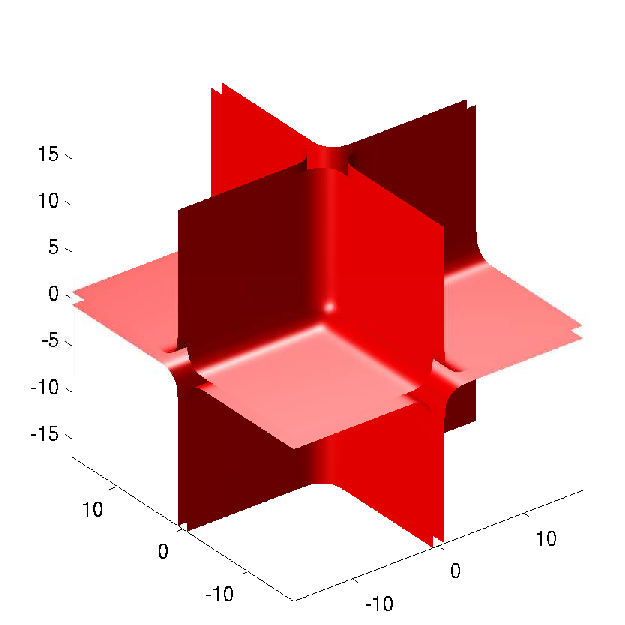
\includegraphics[trim=1em 0em 1em 0em, clip, width=0.25\textwidth]{\additivefigsdir/3d-kernel/3d_add_kernel_1} &
\hspace{-0.2in} 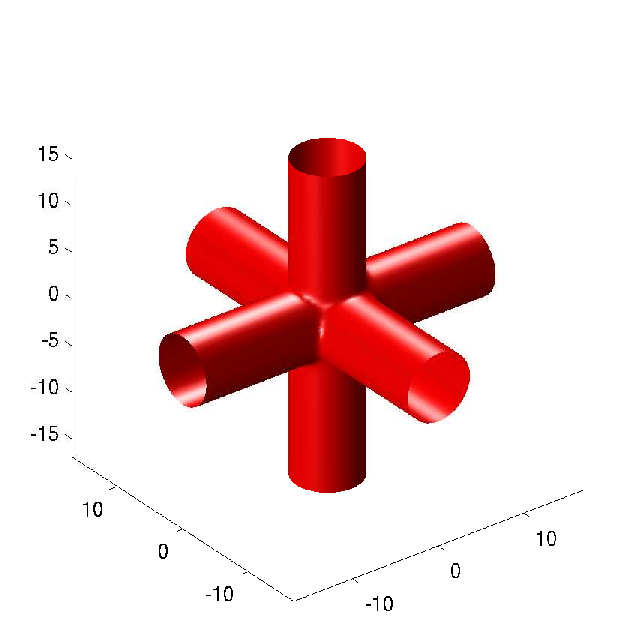
\includegraphics[trim=1em 0em 1em 0em, clip, width=0.25\textwidth]{\additivefigsdir/3d-kernel/3d_add_kernel_2} &
\hspace{-0.2in} 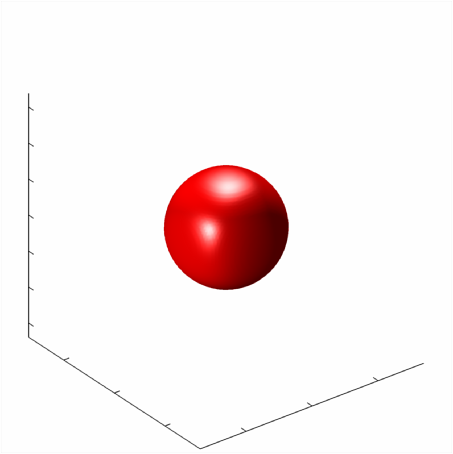
\includegraphics[trim=1em 0em 1em 0em, clip, width=0.25\textwidth]{\additivefigsdir/3d-kernel/3d_add_kernel_3} & 
\hspace{-0.2in} 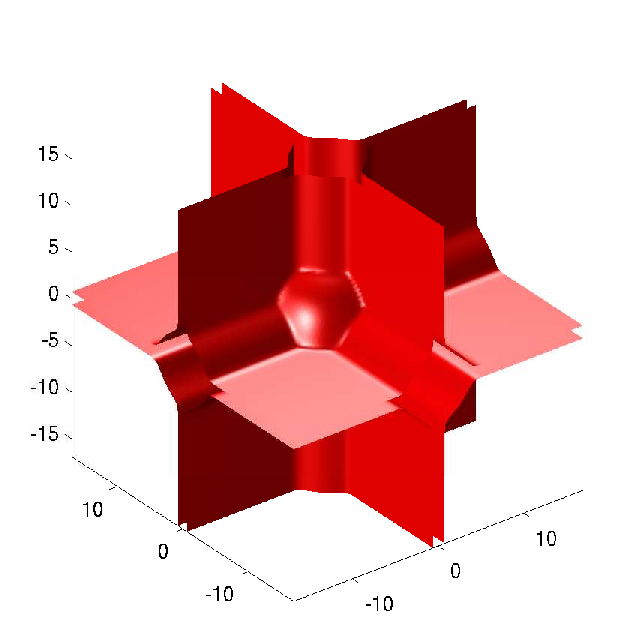
\includegraphics[trim=1em 0em 1em 0em, clip, width=0.25\textwidth]{\additivefigsdir/3d-kernel/3d_add_kernel_321}\\
1st-order terms &
2nd-order terms & 
3rd-order terms & 
All interactions \\
$k_1 + k_2 + k_3$ & $k_1k_2 + k_2k_3 + k_1k_3$ & $k_1k_2k_3$ & \\
& & Squared-exp kernel & Additive kernel\\
\end{tabular}
\caption[Isocontours of additive kernels in 3 dimensions]
{Isocontours of additive kernels in 3 dimensions.
The third-order kernel only considers nearby points relevant, while the lower-order kernels allow the output to depend on distant points, as long as they share one or more input value.}
\label{fig:kernels3d}
\end{figure}

Additive kernels have a much more complex structure, and allow extrapolation based on distant parts of the input space, without spreading the mass of the kernel over the whole space.  For example, additive kernels of the second order allow strong non-local interactions between any points which are similar in any two input dimensions.
\Cref{fig:kernels3d} provides a geometric comparison between squared-exponential kernels and additive kernels in 3 dimensions.

In \cref{ch:kernels}, \cref{sec:additivity-multiple-dimensions} gives an example of how additive kernels extrapolate differently than local kernels.


\section{Dropout in Gaussian Processes}

Dropout is a method for regularizing neural networks \citep{hinton2012improving, srivastava2013improving}.
Training with dropout entails randomly and independently ``dropping'' (setting to zero) some proportion $p$ of features or inputs, in order to improve the robustness of the resulting network by reducing co-dependence between neurons.
To maintain similar overall activation levels, weights are multiplied by $\nicefrac{1}{p}$ at test time. Alternatively, feature activations are multiplied by $\nicefrac{1}{p}$ during training.
At test time, the set of models defined by all possible ways of dropping-out neurons is averaged over, usually in an approximate way.

\citet{baldi2013understanding} and \citet{wang2013fast} analyzed dropout in terms of the effective prior induced by this procedure in several models, such as linear and logistic regression.
In this section, we examine the priors on functions that result from performing dropout in the one-hidden-layer neural network implicitly defined by a \gp{}.

Recall that \gp{}s can be derived as an infinitely-wide one-layer neural network, with fixed activation functions $\feat(\vx)$, and independent random weights $\valpha$ with finite variance $\sigma^2_{\valpha}$:
%
\begin{align}
& f(\vx) = \frac{1}{K}{\mathbf \vnetweights}\tra \hPhi(\vx) = \frac{1}{K} \sum_{i=1}^K \netweights_i \hphi_i(\vx)
\\
\implies & f(\vx) \distas{K \to \infty} \GPt{\expectargs{}{\valpha\tra \feat(\vx)}}{\sigma^2_{\valpha} \feat(\vx)\tra\feat(\vx')}
\label{eq:one-layer-gp-two}
\end{align}
%
Mercer's theorem implies that we can write any \gp{} prior equivalently in this way.
Now that we've expressed a \gp{} as a neural network, we can examine the prior we get from performing dropout in this network.

\subsection{Dropout on Hidden Units}

First, we'll examine the prior we get from independently dropping features from $\hPhi(\vx)$ by setting some of the weights $\valpha$ to zero with probability $p$.
For simplicity, we'll assume that $\expectargs{}{\valpha} = \vzero$.
If the weights initially have finite variance $\sigma^2_{\alpha}$ before dropout, then after dropout they'll have variance
%$\expectargs{}{ \alpha_i} = \vzero, 
%\varianceargs{}{\alpha_i} = \sigma^2$,
%then the distribution of weights after each one has been dropped out with probability $p$ is:
\begin{align}
r_i \simiid \textnormal{Ber}(p)
\qquad
%\expectargs{}{ r_i \alpha_i} = p\mu, \quad 
\varianceargs{}{r_i \alpha_i} = p \sigma_{\alpha}^2 \;.
\end{align}
%Since only the first two moments of the weight variance matter, the resulting \gp{} remain
Because \cref{eq:one-layer-gp-two} is a result of the central limit theorem, it does not depend on the form of the distribution on $\valpha$, only its mean and variance.
Thus, dropping out features of an infinitely-wide \MLP{} does not change the model at all, except to rescale the output variance, since no individual feature can have more than infinitesimal contribution to the network output.
%If we were to rescale the weights by a factor other than $p^{-1/2}$, we would only rescale the output variance of the model, leaving all other aspects identical.
%Is there a better way to drop out features that would lead to robustness?
Indeed, multiplying all weights by $p^{-1/2}$, the initial variance is restored:
\begin{align}
%\expectargs{}{ \frac{1}{p} r_i \alpha_i } = \frac{p}{p}\mu = \mu, \quad 
\varianceargs{}{ \frac{1}{p^\frac{1}{2}} r_i \alpha_i} = \frac{p}{p} \sigma_{\alpha}^2 = \sigma_{\alpha}^2 \;.
\end{align}
In which case dropout on the hidden units has no effect at all.



\subsection{Dropout on Inputs}

In a \gp{} with kernel ${k(\vx, \vx') = \prod_{d=1}^D k_d(x_d, x_d')}$, exact averaging over all possible ways of dropping out inputs with probability $\nicefrac{1}{2}$ results in a mixture of \gp{}s, each depending on only a subset of the inputs:
\begin{align}
p \left( f(\vx) \right)
= \frac{1}{2^D} \sum_{\vr \in \{0,1\}^D}  \textnormal{\gp} \left(f(\vx) \given 0, \prod_{d=1}^D k_d(x_d, x_d')^{r_d} \right)
\label{eq:dropout-mixture}
\end{align}
We present two results ways to gain intuition about this model.

First, if the kernel on each dimension has the form ${k_d(x_d, x_d') = g \left( \frac{x_d - x_d'}{\lengthscale_d} \right)}$, as does the \kSE{} kernel, then any input dimension can be dropped out by setting its lengthscale $\lengthscale_d$ to $\infty$.
Thus, dropout on the inputs of a \gp{} corresponds to a spike-and-slab prior on lengthscales, with each dimension independently having $w_d = \infty$ with probability $\nicefrac{1}{2}$.

Another way to understand the resulting prior is to note that the dropout mixture \eqref{eq:dropout-mixture} has the same covariance as
\begin{align}
f(\vx) \sim \textnormal{\gp} \left(0, \frac{1}{2^{-2D}} \sum_{\vr \in \{0,1\}^D}  \prod_{d=1}^D k_d(x_d, x_d')^{r_d} \right)
\label{eq:additive-gps}
\end{align}

Therefore, dropout on the inputs to a \gp{} can be approximated by the all-subsets additive kernel.
This suggests an interpretation of additive kernels as an approximation to a mixture of models, each of which depends on only a subset of the input variables.


\section{Related Work}

Since additive models are a relatively natural and easy-to-analyze model class, the literature on similar model classes is extensive.
We try to give a broad overview in this section.

\subsubsection{Additive \sgp{}s}

Since the non-local structure capturable by additive kernels is necessarily axis-aligned, we can naturally consider that an initial transformation of the input space might allow us to recover non-axis aligned additivity in functions.
This avenue was explored by \citet{gilboa2013scaling}, who developed a linearly-transformed first-order additive \gp{} model, called projection-pursuit \gp{} regression.  They further showed that inference in this model was possible in $\mathcal{O}(N)$ time.

\citet{durrande2011additive} also examined the properties of additive \gp{}s, and proposed a layer-wise optimization strategy for kernel hyperparameters in these models.

\citet{plate1999accuracy} constructed an additive \gp{} using only the first-order and $D$th-order terms.
This model is motivated by the desire to trade off the interpretability of first-order models with the flexibility of full-order models.
Our experiments show that often, the intermediate degrees of interaction contribute most of the variance.

A related functional \ANOVA{} \gp{} model \citep{kaufman2010bayesian} decomposes the \emph{mean} function into a weighted sum of \gp{}s.
However, the effect of a particular degree of interaction cannot be quantified by that approach.
Also, computationally, the Gibbs sampling approach used in \citep{kaufman2010bayesian} is disadvantageous.
%[TODO: read and mention \citep{friedman1981projection} from Hannes]

\citet{christoudias2009bayesian} previously showed how mixtures of kernels can be learnt by gradient descent in the Gaussian process framework.
They call this \emph{Bayesian localized multiple kernel learning}.
However, their approach learns a mixture over a small, fixed set of kernels, while our method learns a mixture over all possible products of those kernels.


\subsubsection{Hierarchical Kernel Learning}

A similar model class was recently explored by \citet{DBLP:journals/corr/abs-0909-0844} called Hierarchical Kernel Learning (\HKL{}).
%Finally, on real datasets, HKL is outperformed by the standard \SEGP{} \citep{DBLP:journals/corr/abs-0909-0844}.
\HKL{} uses a regularized optimization framework to learn a weighted sum over an exponential number of kernels which can be computed in polynomial time.
%
\begin{figure}[ht!]
\centering
\begin{tabular}{c|c}
Hierarchical Kernel Learning & All-orders additive \gp{} \\
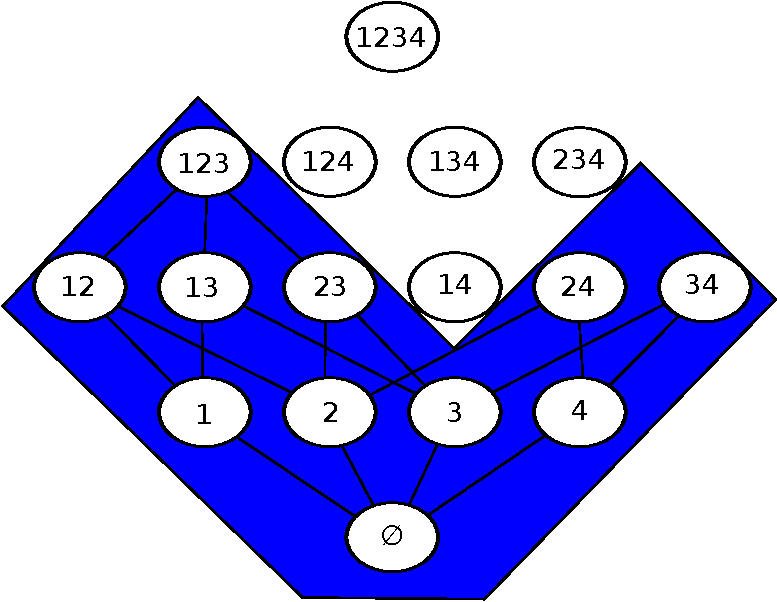
\includegraphics[height=0.35\textwidth]{\additivefigsdir/compare_models/hkl.pdf} &
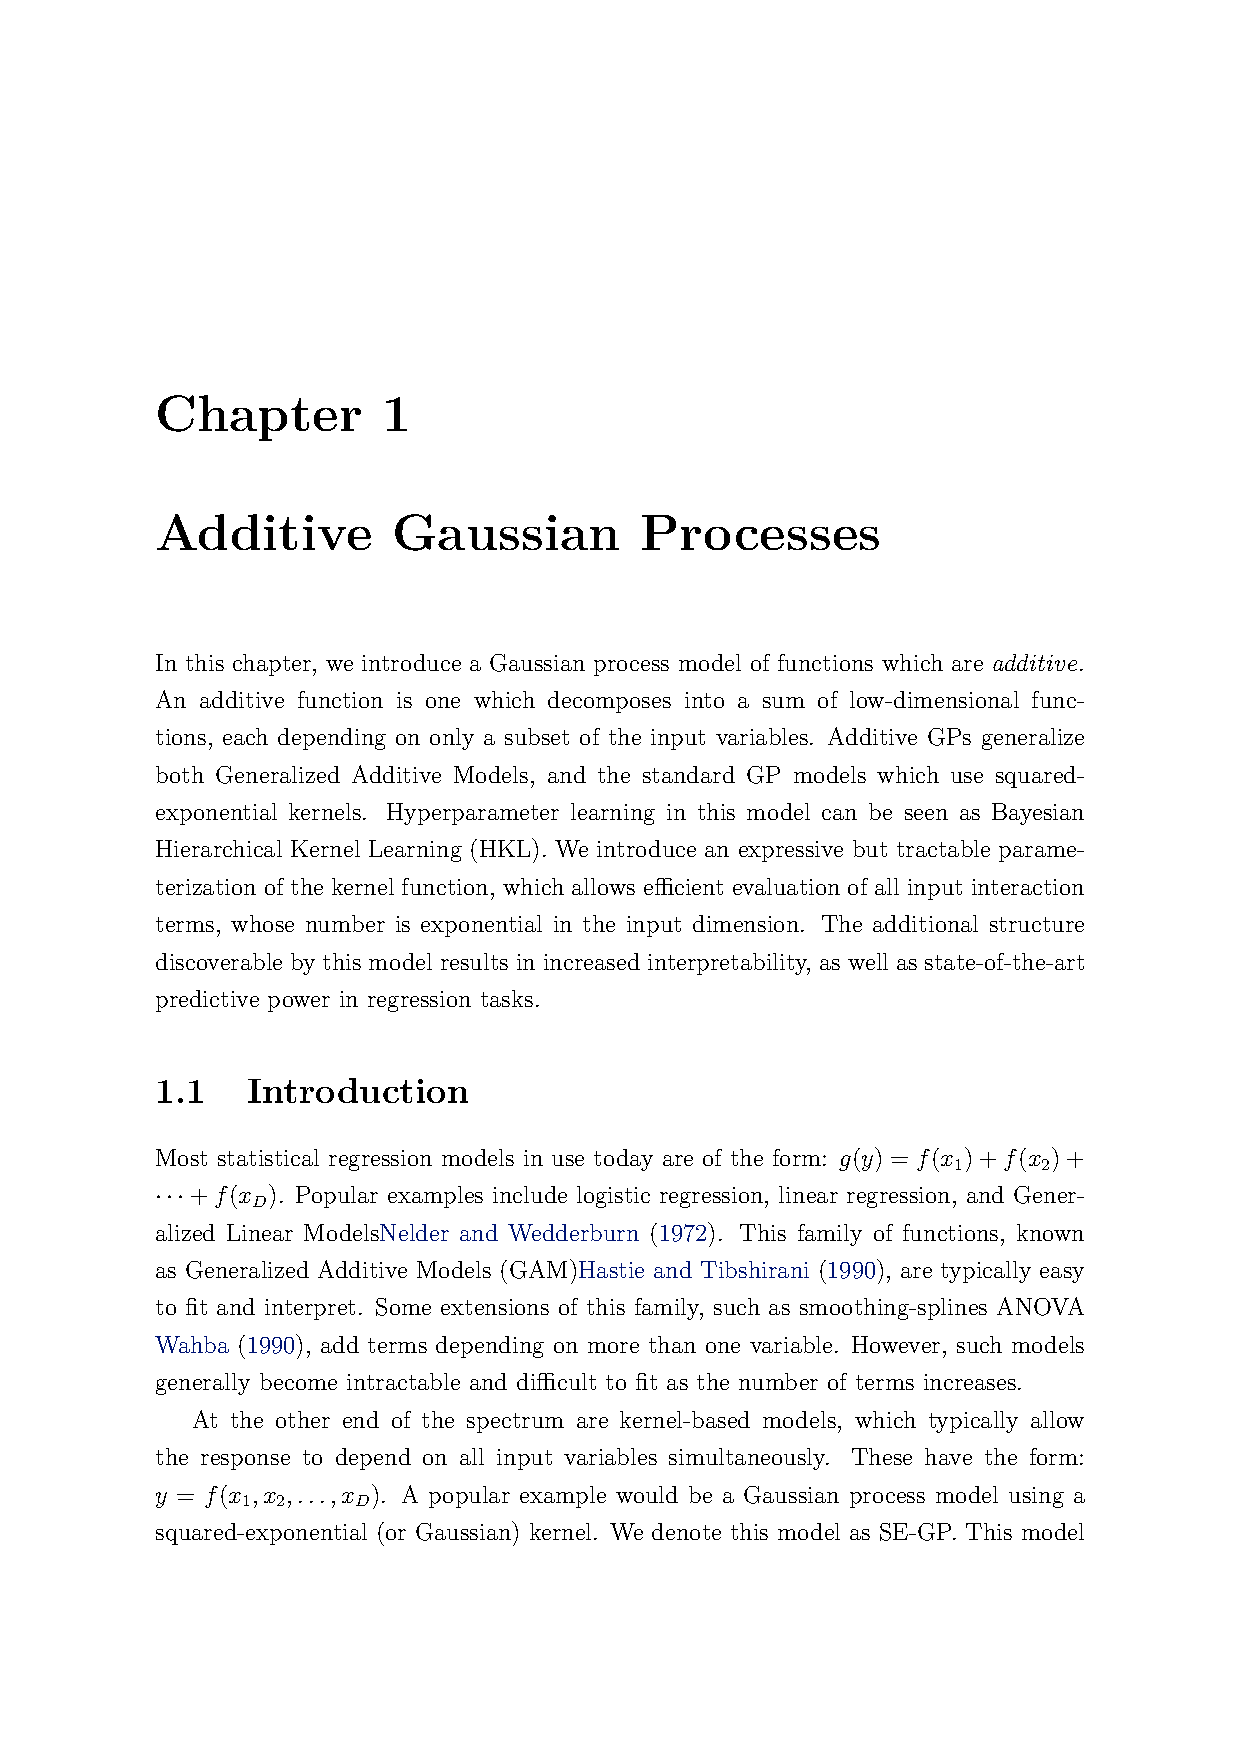
\includegraphics[height=0.35\textwidth]{\additivefigsdir/compare_models/additive.pdf}
\\ \hline \\
 Squared-exp GP & First-order additive \gp{} \\
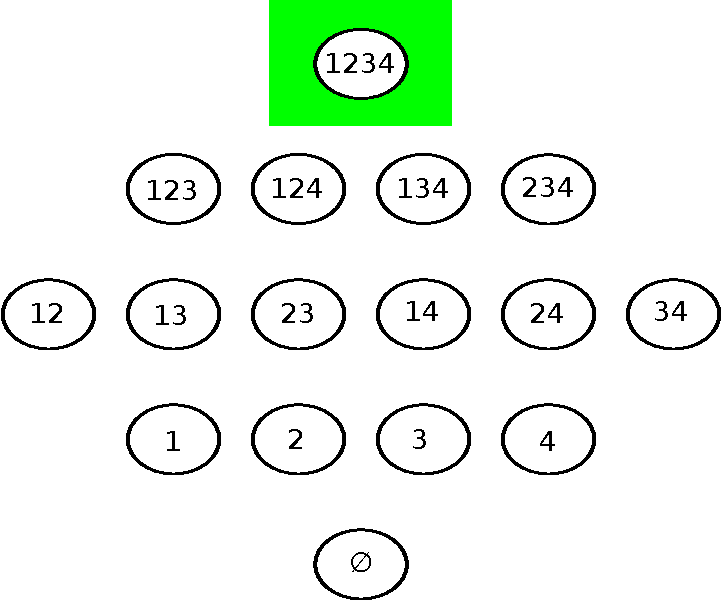
\includegraphics[height=0.35\textwidth]{\additivefigsdir/compare_models/ard.pdf} &
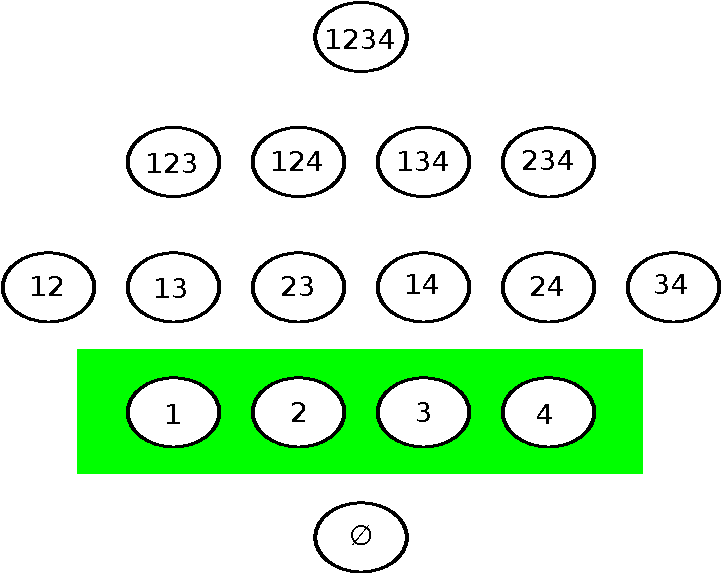
\includegraphics[height=0.35\textwidth]{\additivefigsdir/compare_models/gam.pdf} \\
\end{tabular}
\caption[A comparison of different additive model classes]
{
%A comparison of model flexibility between HKL, additive GPs, the GP-Generalized Additive Model, and the squared-exponential GP model.  
A comparison of different additive model classes.
Nodes represent different interaction terms, ranging from first-order to fourth-order interactions.
Coloured boxes represent the weightings of different terms.
\emph{Top left: }\HKL{} can select a hull of interaction terms, but must use a pre-determined weighting over those terms.
\emph{Top right:} the additive \gp{} model can weight each order of interaction separately.
\emph{Bottom row:} Neither \HKL{} nor the additive model dominate one another in terms of flexibility, however the \SEGP{} and first-order additive \gp{} models are special cases of the all-orders additive \gp{}. }
\label{hulls-figure}
\end{figure}
%
This method chooses among \textit{hull} of kernels, defined as a subset of all terms such that if $\prod_{j \in J} k_j(\bf x, x')$ is included in the subset, then so are all terms $\prod_{j \in J / i} k_j(\bf x, x')$, for all $i \in J$.
%For details, see \citep{DBLP:journals/corr/abs-0909-0844}.
%Given each dimension's kernel, and a pre-defined weighting over all terms, \HKL{} performs model selection by searching over hulls of interaction terms.
% \subsubsection{All-subsets kernel with uniform weightings}
%\citet{DBLP:journals/corr/abs-0909-0844} fixes the relative weighting between orders of interaction with a single term $\alpha$, 
\HKL{} computes the sum over all orders in $\mathcal{O}(D)$ time by the formula:
\begin{equation}
\label{eqn:uniform}
k_{a}({\bf x, x'}) = v^2 \prod_{d=1}^D \left(1 + \alpha k_{d}(x_{d}, x_{d}') \right)
\end{equation}
%which has computational complexity .
%However, this formulation 
which forces the weight of all $n$th order terms to be weighted by $\alpha^n$.


Figure~\ref{hulls-figure} contrasts the \HKL{} model class with the additive \gp{} model.
Neither method is strictly more flexible than the other.
The main difficulty with the approach of \citet{DBLP:journals/corr/abs-0909-0844} is that the kernel parameters are hard to set, other than by cross-validation.
%In contrast, our method optimizes the parameters of each dimension's base kernel, as well as the relative weighting of each order of interaction. 


\subsubsection{Support Vector Machines}

\citet{vapnik1998statistical} introduced the support vector \ANOVA{} decomposition, which has the same form as our additive kernel.
They recommend approximating the sum over all $D$ orders with only one term ``of appropriate order'', presumably because of the difficulty of setting the parameters of an \SVM{}.
\citet{stitson1999support} performed experiments which favourably compared the predictive accuracy of the support vector \ANOVA{} decomposition against polynomial and spline kernels.
They too allowed only one order to be active, and set parameters by cross-validation.
%
%  The order of the kernel, kernel parameters, the allowable regression error $\epsilon$, and the cost hyperparameter $c$ were all set by a lengthy cross-validation process.

%\subsection{Smoothing Splines ANOVA}
\subsubsection{Other Related Models}

A closely related procedure from \citet{wahba1990spline} is smoothing-splines \ANOVA{} (\SSANOVA{}).
An \SSANOVA{} model is a weighted sum of splines along each dimension, plus a sum of splines over all pairs of dimensions, all triplets, etc, with each individual interaction term having a separate weighting parameter.
Because the number of terms to consider grows exponentially in the order, in practice, only terms of first and second order are usually considered.
%Learning in SS-ANOVA is usually done via penalized-maximum likelihood with a fixed sparsity hyperparameter.
%\citep{shawe2004kernel} define ANOVA kernels thusly: "The ANOVA kernel of degree d is like the all-subsets kernel except that it is restricted to subsets of the given cardinality $d$."

% estimated by generalized cross-validation\citep{craven1978smoothing}. 
%MARS\citep{friedman1991multivariate} is another spline-based regression method.

This more general model class, in which each interaction term is estimated separately, is known in the physical sciences as High Dimensional Model Representation (\HDMR{}).
\citet{rabitz1999general} review some properties and applications of this model class.

The main benefits of the model setup and parameterization proposed in this chapter are the ability to include all $D$ orders of interaction with differing weights, and the ability to learn kernel parameters individually per input dimension, allowing automatic relevance determination to operate.



\section{Experiments}
\label{sec:additive-experiments}

\subsubsection{Parameterization}
A $D$-dimensional \kSE-\ARD{} kernel has $D$ lengthscale parameters and the output variance.
An first-order additive $\kSE$ model has $2 \times D$ parameters.
A fully-parametrized model including all orders of interaction, with a separate output variance for each scale will have $3 \times D$ parameters.
Because each additional parameter increases the tendency to overfit, we recommend allowing only one kernel parameter per input dimension. 
%
%Since there always exists a parameterization of the additive function corresponding to the product kernel, we initialize the hyperparameter search for the additive kernel by first learning parameters for the equivalent product kernel.  This ensures that we start our search in a reasonable area of hyperparameter space.
%
In our experiments, we parametrized each one-dimensional kernel with only the lengthscale, fixing the output variance to be 1.

\subsubsection{Methods}

%On a diverse collection of datasets, 
We compare six different methods.
In the results tables below, \gp{} Additive refers to a \gp{} using the additive kernel with squared-exp base kernels.
For speed, we limited the maximum order of interaction in the additive kernels to 10.
\gp{}-1st denotes an additive \gp{} model with only first-order interactions - a sum of one-dimensional kernels.
\gp{} Squared-Exp is a \gp{} model with a squared-exponential \ARD{} kernel.
\HKL{} was run using the all-subsets kernel, which corresponds to the same set of kernels as considered by the additive \gp{} with a squared-exp base kernel.

For all \gp{} models, we fit kernel parameters by the standard method of maximizing training-set marginal likelihood, using \LBFGS{} \citep{nocedal1980updating} for 500 iterations, allowing five random restarts.
In addition to learning kernel parameters, we fit a constant mean function to the data.
In the classification experiments, approximate \gp{} inference was done using Expectation Propagation \citep{minka2001expectation}.

For the regression experiments, we also compared against the structure search method from \cref{ch:grammar}, run up to depth 10, using the \SE{} and \RQ{} base kernel families.

\subsection{Datasets}

We compared these methods on a diverse set of regression and classification datasets from the UCI repository~\citep{UCI}.  Their size and dimension are given in \cref{table:regression-dataset-stats,table:classification-dataset-stats}:

\begin{table}[h]
\caption{Regression Dataset Statistics}
\label{tbl:Regression Dataset Statistics}
\begin{center}
\begin{tabular}{l | lllll}
Method & bach & concrete & pumadyn & servo & housing \\ \hline
Dimension      & 8    & 8        & 8       & 4     & 13 \\
Number of datapoints       & 200  & 500      & 512     & 167   & 506
\end{tabular}
\end{center}
\label{table:regression-dataset-stats}
\end{table}
%
\begin{table}[h]
\caption{Classification Dataset Statistics}
\label{tbl:Classification Dataset Statistics}
\begin{center}
\begin{tabular}{l | llllll}
Method & breast & pima & sonar & ionosphere & liver & heart\\ \hline
Dimension      & 9      & 8    & 60    & 32         & 6     & 13 \\
Number of datapoints      & 449    & 768  & 208   & 351        & 345   & 297
\end{tabular}
\end{center}
\label{table:classification-dataset-stats}
\end{table}

\subsubsection{Bach Synthetic Dataset}
In addition to standard UCI repository datasets, we generated a synthetic dataset following the same recipe as \citet{DBLP:journals/corr/abs-0909-0844}.
This dataset was designed to demonstrate the advantages of \HKL{} over \gp{}-\SE{}.
%From a covariance matrix drawn from a Wishart distribution with 1024 degrees of freedom, we select 8 variables.
It is generated by passing correlated Gaussian-distributed inputs $x_1, x_2, \dots, x_8$ through the quadratic function
%
\begin{align}
f(\vx) = \sum_{i=1}^4 \sum_{j=1+1}^4 x_i x_j + \epsilon \qquad \epsilon \sim \Nt{0}{\sigma_\epsilon}
\end{align}
%
%which sums all 2-way products of the first 4 variables, and adds Gaussian noise $\epsilon$.
This dataset is well-modeled by an additive kernel which includes all two-way interactions over the first 4 variables, but does not depend on the extra 4 irrelevant inputs.%, as well as the higher-order interactions.
%TODO: Move description to grammar experiments?

If the dataset is large enough, \HKL{} can construct a hull around only the 16 cross-terms optimal for predicting the output.
\gp{}-\SE{}, in contrast, can learn to ignore the noisy copy variables, but cannot learn to ignore the higher-order interactions between dimensions.
However, a \gp{} with an additive kernel can learn both to ignore irrelevant variables, and to ignore missing orders of interaction.
With enough data, the marginal likelihood will favour hyperparameters specifying such a model.
%In this example, the additive \gp{} is able to recover the relevant structure.
 
 
\subsection{Results}
\Cref{tbl:Regression Mean Squared Error,tbl:Regression Negative Log Likelihood,tbl:Classification Percent Error,tbl:Classification Negative Log Likelihood} show mean performance across 10 train-test splits.
Because \HKL{} does not specify a noise model, it could not be included in the likelihood comparisons.

% --- Automatically generated by resultsToLatex2.m ---
% Exported at 19-Jan-2012 10:55:19
\begin{table}[h!]
\caption[Comparison of predictive error on regression problems]
{Regression Mean Squared Error}
\label{tbl:Regression Mean Squared Error}
\begin{center}
\begin{tabular}{l | r r r r r}
Method & \rotatebox{0}{ bach  }  & \rotatebox{0}{ concrete  }  & \rotatebox{0}{ pumadyn-8nh }  & \rotatebox{0}{ servo }  & \rotatebox{0}{ housing }  \\ \hline
Linear Regression & $1.031$ & $0.404$ & $0.641$ & $0.523$ & $0.289$ \\
\gp{}-1st & $1.259$ & $0.149$ & $0.598$ & $0.281$ & $0.161$ \\
\HKL{} & $\mathbf{0.199}$ & $0.147$ & $0.346$ & $0.199$ & $0.151$ \\
\gp{} Squared-exp & $\mathbf{0.045}$ & $0.157$ & $0.317$ & $0.126$ & $\mathbf{0.092}$ \\
\gp{} Additive & $\mathbf{0.045}$ & $\mathbf{0.089}$ & $\mathbf{0.316}$ & $\mathbf{0.110}$ & $0.102$ \\
Structure Search & $\mathbf{0.044}$ & $\mathbf{0.087}$ & $\mathbf{0.315}$ & $\mathbf{0.102}$ & $\mathbf{0.082}$
\end{tabular}
\end{center}
\end{table}
% End automatically generated LaTeX
%
% --- Automatically generated by resultsToLatex2.m ---
% Exported at 19-Jan-2012 10:55:19
\begin{table}[h!]
\caption[Comparison of predictive likelihood on regression problems]
{Regression Negative Log Likelihood}
\label{tbl:Regression Negative Log Likelihood}
\begin{center}
\begin{tabular}{l | r r r r r}
Method & \rotatebox{0}{ bach  }  & \rotatebox{0}{ concrete  }  & \rotatebox{0}{ pumadyn-8nh }  & \rotatebox{0}{ servo }  & \rotatebox{0}{ housing }  \\ \hline
Linear Regression & $2.430$ & $1.403$ & $1.881$ & $1.678$ & $1.052$ \\
\gp{}-1st & $1.708$ & $0.467$ & $1.195$ & $0.800$ & $0.457$ \\
GP Squared-exp & $\mathbf{-0.131}$ & $0.398$ & $0.843$ & $0.429$ & $0.207$ \\
GP Additive & $\mathbf{-0.131}$ & $\mathbf{0.114}$ & $\mathbf{0.841}$ & $\mathbf{0.309}$ & $0.194$ \\
Structure Search & $\mathbf{-0.141}$ & $\mathbf{0.065}$ & $\mathbf{0.840}$ & $\mathbf{0.265}$ & $\mathbf{0.059}$
\end{tabular}
\end{center}
\end{table}
% End automatically generated LaTeX
%
% --- Automatically generated by resultsToLatex2.m ---
% Exported at 03-Jun-2011 00:23:25
\begin{table}[h!]
\caption[Comparison of predictive error on classification problems]
{Classification percent error}
\label{tbl:Classification Percent Error}
\begin{center}
\begin{tabular}{l | r r r r r r}
Method & \rotatebox{0}{ breast }  & \rotatebox{0}{ pima }  & \rotatebox{0}{ sonar }  & \rotatebox{0}{ ionosphere }  & \rotatebox{0}{ liver }  & \rotatebox{0}{ heart }  \\ \hline
Logistic Regression & $7.611$ & $24.392$ & $26.786$ & $16.810$ & $45.060$ & $\mathbf{16.082}$ \\
\gp{}-1st & $\mathbf{5.189}$ & $\mathbf{22.419}$ & $\mathbf{15.786}$ & $\mathbf{8.524}$ & $\mathbf{29.842}$ & $\mathbf{16.839}$ \\
\HKL{} & $\mathbf{5.377}$ & $24.261$ & $\mathbf{21.000}$ & $9.119$ & $\mathbf{27.270}$ & $\mathbf{18.975}$ \\
\gp{} Squared-exp & $\mathbf{4.734}$ & $\mathbf{23.722}$ & $\mathbf{16.357}$ & $\mathbf{6.833}$ & $\mathbf{31.237}$ & $\mathbf{20.642}$ \\
\gp{} Additive & $\mathbf{5.566}$ & $\mathbf{23.076}$ & $\mathbf{15.714}$ & $\mathbf{7.976}$ & $\mathbf{30.060}$ & $\mathbf{18.496}$ \\
\end{tabular}
\end{center}
\end{table}
% End automatically generated LaTeX
%
% --- Automatically generated by resultsToLatex2.m ---
% Exported at 03-Jun-2011 00:23:28
\begin{table}[h!]
\caption[Comparison of predictive likelihood on classification problems]
{Classification negative log-likelihood}
\label{tbl:Classification Negative Log Likelihood}
\begin{center}
\begin{tabular}{l | r r r r r r}
Method & \rotatebox{0}{ breast }  & \rotatebox{0}{ pima }  & \rotatebox{0}{ sonar }  & \rotatebox{0}{ ionosphere }  & \rotatebox{0}{ liver }  & \rotatebox{0}{ heart }  \\ \hline
Logistic Regression & $0.247$ & $0.560$ & $4.609$ & $0.878$ & $0.864$ & $0.575$ \\
\gp{}-1st & $\mathbf{0.163}$ & $\mathbf{0.461}$ & $\mathbf{0.377}$ & $\mathbf{0.312}$ & $\mathbf{0.569}$ & $\mathbf{0.393}$ \\
\gp{} Squared-exp & $\mathbf{0.146}$ & $0.478$ & $\mathbf{0.425}$ & $\mathbf{0.236}$ & $\mathbf{0.601}$ & $0.480$ \\
\gp{} Additive & $\mathbf{0.150}$ & $\mathbf{0.466}$ & $\mathbf{0.409}$ & $\mathbf{0.295}$ & $\mathbf{0.588}$ & $\mathbf{0.415}$ \\
\end{tabular}
\end{center}
\end{table}
% End automatically generated LaTeX

The model with best performance on each dataset is in bold, along with all other models that were not significantly different under a paired $t$-test.
%The additive model never performs significantly worse than any other model, and sometimes performs significantly better than all other models.
The additive and structure search methods usually outperformed the other methods, especially on regression problems.
The structure search outperforms the additive \gp{}, but at the cost of a slow search over kernels.

%The difference between all methods is larger in the case of regression experiments.

The additive \gp{} performed best on datasets well-explained by low orders of interaction, and approximately as well as the \SE{}-\gp{} model on datasets which were well explained by high orders of interaction (see \cref{tbl:all_orders}).
Because the additive \gp{} is a superset of both the \gp{}-1st model and the \kSE{}-\gp{} model, instances where the additive \gp{} performs slightly worse are presumably due to over-fitting, or due to the hyperparameter optimization becoming stuck in a local maximum. % Absence of over-fitting may explain the relatively strong performance of GP-GAM on classification tasks.  
Performance could be expected to benefit from approximately integrating over the kernel parameters.

The performance of \HKL{} is consistent with the results in \citep{DBLP:journals/corr/abs-0909-0844}, performing competitively but slightly worse than \SE{}-\gp{}.%  This is especially clear in the case of the regression tasks.


\subsection{Source Code}
Additive Gaussian processes are particularly appealing in practice because their use requires only the specification of the base kernel; all other aspects of \gp{} inference remain the same.
Note that we are also free to choose a different covariance function along each dimension.

All of the experiments in this chapter were performed using the standard \GPML{} toolbox, available at \url{http://www.gaussianprocess.org/gpml/code/}.
Code to perform all experiments is available at \url{http://github.com/duvenaud/additive-gps}





\section{Conclusion}

%We present a simple model which generalizes two widely-used classes of models.  A large increase in modeling power is gained at only modest computational cost.
In this chapter, we presented a parameterization of higher-order additive \gp{}s allowing for tractable inference.
%This a simple family of models which generalizes two widely-used classes of models.
%Additive \gp{}s also introduce a tractable new type of structure into the \gp{} framework.
Our experiments indicate that, to varying degrees, additive structure is present in real datasets.
When it is present, modeling this structure allows our model to perform better than standard \gp{} models.
In the case where no such structure exists, the higher-order interaction terms present in the kernel can recover arbitrarily flexible models, as well.

The additive \gp{} also affords extra interpretability: the variance parameters on each order of interaction indicate which sorts of structure are present the data.

%Compared to \HKL{}, which is the only other tractable procedure able to capture the same types of structure, our method benefits from being able to learn individual kernel parameters, as well as the weightings of different orders of interaction.
%Our experiments show that additive \gp{}s are a state-of-the-art regression model.



\outbpdocument{
\bibliographystyle{plainnat}
\bibliography{references.bib}
}





%\begin{figure}
%\centering
%\begin{tabular}{cc}
%\hspace{-0.1in}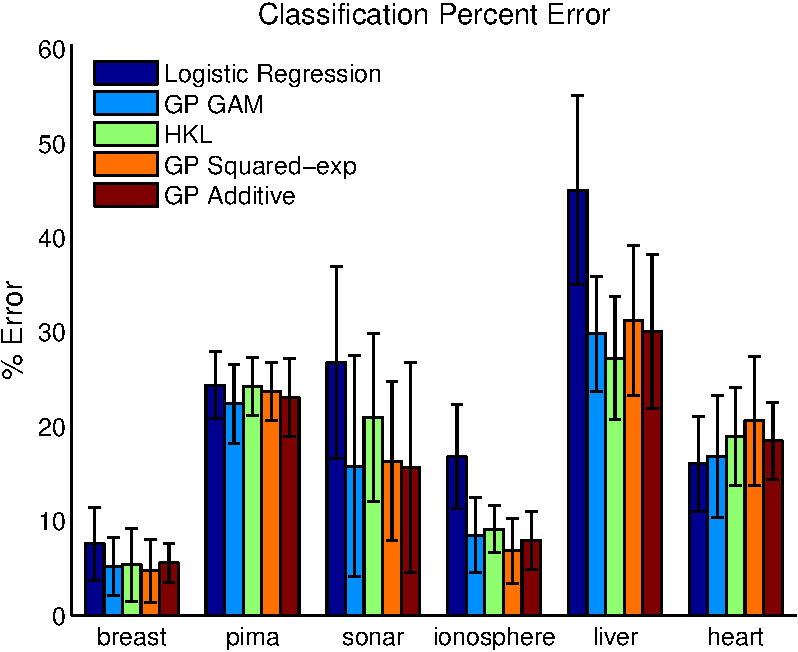
\includegraphics[width=0.475\textwidth]{\additivefigsdir/class_graph.pdf} &
%\hspace{-0.1in}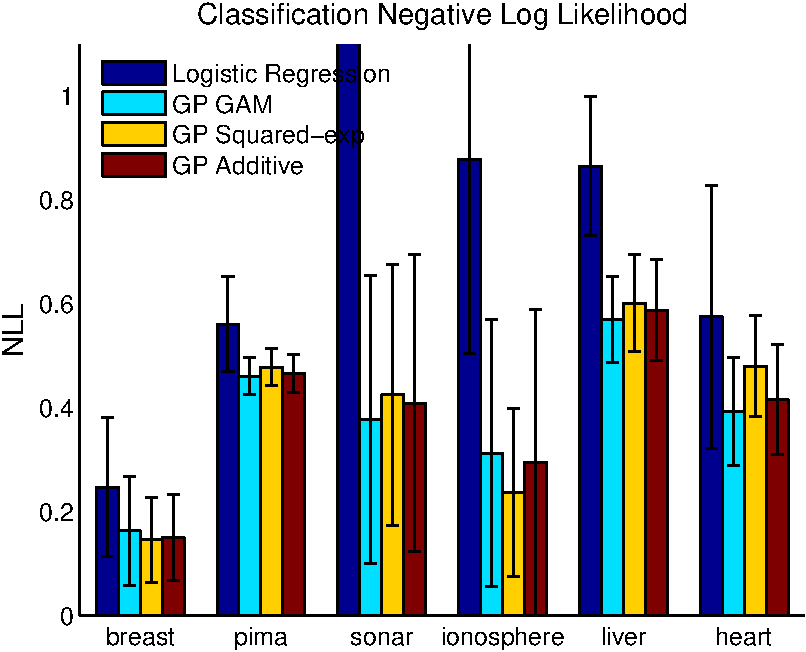
\includegraphics[width=0.475\textwidth]{\additivefigsdir/class_graph_ll.pdf}\\
%\hspace{-0.1in}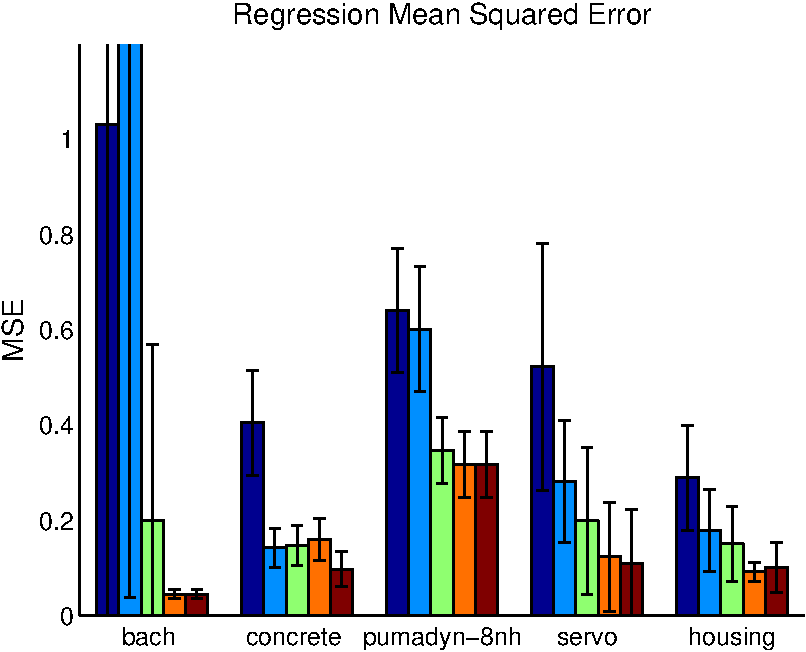
\includegraphics[width=0.475\textwidth]{\additivefigsdir/reg_graph.pdf}& 
%\hspace{-0.1in}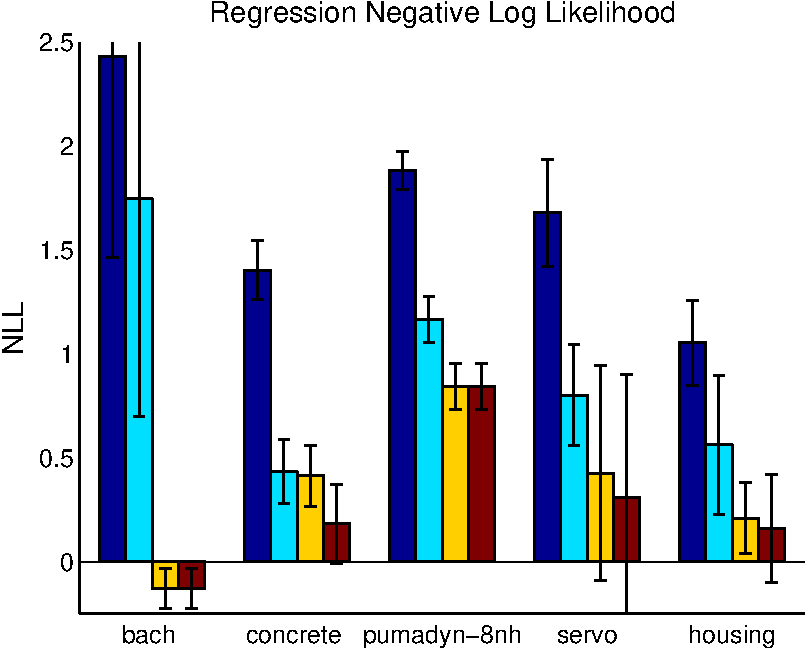
\includegraphics[width=0.475\textwidth]{\additivefigsdir/reg_graph_ll.pdf}\\ 
%\end{tabular}
%\label{fig:results}
%\end{figure}


%\section{Discussion}
%% --- Automatically generated by hypers_to_latex.m ---
% Exported at 12-May-2011 16:56:21
\begin{table}[h]
\caption{{\small
Hyperparameters for housing dataset
}}
\label{tbl:housing}
\begin{center}
\begin{tabular}{l | r r r r r r r r r r r r r}
Variable: & $x_1$  & $x_2$  & $x_3$  & $x_4$  & $x_5$  & $x_6$  & $x_7$  & $x_8$  & $x_9$  & $x_10$  & $x_11$  & $x_12$  & $x_13$  \\ \hline
ARD Lengthscale & $1508.26$  & $504.64$  & $296.62$  & $3.91$  & $0.08$  & $2.21$  & $5.77$  & $2.77$  & $424.77$  & $0.74$  & $233.78$  & $605.23$  & $3.75$  \\ 
\hline
ADD Lengthscale & $392.41$  & $147.62$  & $183.48$  & $12.16$  & $0.04$  & $2.33$  & $5.71$  & $0.49$  & $402.78$  & $0.68$  & $322.01$  & $1027.36$  & $1.48$  \\
ADD Variance & $0.29$ & $0.29$ & $0.29$ & $0.44$ & $0.02$ & $19.14$ & $0.25$ & $0.97$ & $0.29$ & $10.77$ & $0.29$ & $0.29$ & $0.37$ \\ \hline
Order of Interaction: & \nth{1} & \nth{2} & \nth{3} & \nth{4} & \nth{5} & \nth{6} & \nth{7} & \nth{8} & \nth{9} & \nth{10} \\
ADD Order Variance & $0.1$\% & $0.1$\% & $0.1$\% & $0.0$\% & $0.0$\% & $0.0$\% & $0.0$\% & $0.0$\% & $0.0$\% & $99.8$\% \\ \hline
\end{tabular}
\end{center}
\end{table}
% End automatically generated LaTeX

%% --- Automatically generated by hypers_to_latex.m ---
% Exported at 12-May-2011 16:56:20
\begin{table}[h]
\caption{{\small
Hyperparameters for pima dataset
}}
\label{tbl:pima}
\begin{center}
\begin{tabular}{l | r r r r r r r r}
Variable: & $x_1$  & $x_2$  & $x_3$  & $x_4$  & $x_5$  & $x_6$  & $x_7$  & $x_8$  \\ \hline
ARD Lengthscale & $0.30$  & $0.05$  & $4.15$  & $3.62$  & $0.26$  & $1.78$  & $326.52$  & $0.76$  \\ 
\hline
ADD Lengthscale & $0.23$  & $0.05$  & $3.75$  & $6.37$  & $0.27$  & $1.81$  & $107.98$  & $0.58$  \\
ADD Variance & $2.47$ & $0.03$ & $0.86$ & $0.75$ & $0.35$ & $1.56$ & $0.71$ & $60.36$ \\ \hline
Order of Interaction: & \nth{1} & \nth{2} & \nth{3} & \nth{4} & \nth{5} & \nth{6} & \nth{7} & \nth{8} \\
ADD Order Variance & $0.0$\% & $0.1$\% & $0.1$\% & $0.3$\% & $0.0$\% & $29.0$\% & $0.1$\% & $70.4$\% \\ \hline
\end{tabular}
\end{center}
\end{table}
% End automatically generated LaTeX



%As a special case, additive kernels with only one degree of interaction can be computed in something like linear time [cite Yunus?]
 % E = elsympol(Kd(:,:,[1:j-1,j+1:D]),max(R)-1);



 
 
%\subsection{Polynomial Kernels}

%A simple variation on the all-subsets kernel would be one which includes repeated terms, of the form
%\begin{equation}
%k_{h_n}({\bf x, x'}) = v_n^2 \sum_{i_1, \dots, i_n} \prod_{d=1}^n k_{i_d}(x_{i_d}, x_{i_d}') = v_n^2 \prod_{d=1}^n \sum_{i_1, \dots, i_n}^n k_{i_d}(x_{i_d}, x_{i_d}')
%\end{equation}
%This formulation allows repeated terms, such as $x_i^2$ and is equivalent to the polynomial kernel\citep{shawe2004kernel}.  However, this formulation cases the length scale of each dimension to vary with the order of interaction considered.




%[Equation for derivatives]





%The fact that our model is additive does not mean that it ignores multiplicative, or higher-order interactions


%
% A header that lets you compile a chapter by itself, or inside a larger document.
% Adapted from http://stackoverflow.com/questions/3655454/conditional-import-in-latex
%
%
%Use \inbpdocument and \outbpdocument in your individual files, in place of \begin{document} and \end{document}. In your main file, put in a \def \ismaindoc {} before including or importing anything.
%
% David Duvenaud
% June 2011
% 
% ======================================
%
%


\ifx\ismaindoc\undefined
	\newcommand{\inbpdocument}{
		\def \ismaindoc {}
		% Use this header if we are compiling by ourselves.
		\documentclass[a4paper,11pt,authoryear,index]{common/PhDThesisPSnPDF}
		
%\usepackage{draftwatermark}
%\SetWatermarkLightness{0.95}

% ******************************************************************************
% ****************************** Custom Margin *********************************

% Add `custommargin' in the document class options to use this section
% Set {innerside margin / outerside margin / topmargin / bottom margin}  and
% other page dimensions

\ifsetMargin
\else
    \RequirePackage[left=37mm,right=30mm,top=35mm,bottom=30mm]{geometry}
    \setFancyHdr % To apply fancy header after geometry package is loaded
\fi


%\chead{Unfinished draft}
%\cfoot{\texttt{Unfinished draft - compiled on \today{} at \currenttime}}

% *****************************************************************************
% ******************* Fonts (like different typewriter fonts etc.)*************

% Add `customfont' in the document class option to use this section

\ifsetFont
\else
    % Set your custom font here and use `customfont' in options. Leave empty to
    % load computer modern font (default LaTeX font).  

    \RequirePackage{libertine} 
\fi

% *****************************************************************************
% *************************** Bibliography  and References ********************

%\usepackage{cleveref} %Referencing without need to explicitly state fig /table

% Add `custombib' in the document class option to use this section
\ifsetBib % True, Bibliography option is chosen in class options
\else % If custom bibliography style chosen then load bibstyle here

   \RequirePackage[square, sort, numbers, authoryear]{natbib} % CustomBib

% If you would like to use biblatex for your reference management, as opposed to the default `natbibpackage` pass the option `custombib` in the document class. Comment out the previous line to make sure you don't load the natbib package. Uncomment the following lines and specify the location of references.bib file

% \RequirePackage[backend=biber, style=numeric-comp, citestyle=numeric, sorting=nty, natbib=true]{biblatex}
% \bibliography{References/references} %Location of references.bib only for biblatex

\fi


% changes the default name `Bibliography` -> `References'
\renewcommand{\bibname}{References}


% *****************************************************************************
% *************** Changing the Visual Style of Chapter Headings ***************
% Uncomment the section below. Requires titlesec package.

%\RequirePackage{titlesec}
%\newcommand{\PreContentTitleFormat}{\titleformat{\chapter}[display]{\scshape\Large}
%{\Large\filleft{\chaptertitlename} \Huge\thechapter}
%{1ex}{}
%[\vspace{1ex}\titlerule]}
%\newcommand{\ContentTitleFormat}{\titleformat{\chapter}[display]{\scshape\huge}
%{\Large\filleft{\chaptertitlename} \Huge\thechapter}{1ex}
%{\titlerule\vspace{1ex}\filright}
%[\vspace{1ex}\titlerule]}
%\newcommand{\PostContentTitleFormat}{\PreContentTitleFormat}
%\PreContentTitleFormat


% *****************************************************************************
% **************************** Custom Packages ********************************
% *****************************************************************************


% ************************* Algorithms and Pseudocode **************************

%\usepackage{algpseudocode} 


% ********************Captions and Hyperreferencing / URL **********************

% Captions: This makes captions of figures use a boldfaced small font. 
%\RequirePackage[small,bf]{caption}

\RequirePackage[labelsep=space,tableposition=top]{caption} 
%\renewcommand{\figurename}{Figure} %to support older versions of captions.sty
\captionsetup{belowskip=12pt,aboveskip=4pt}

% ************************ Formatting / Footnote *******************************

%\usepackage[perpage]{footmisc} %Range of footnote options 


% ****************************** Line Numbers **********************************

%\RequirePackage{lineno}
%\linenumbers

% ************************** Graphics and figures *****************************

%\usepackage{rotating}
%\usepackage{wrapfig}
%\usepackage{float}
\usepackage{subfig} %note: subfig must be included after the `caption` package. 


% ********************************* Table **************************************

%\usepackage{longtable}
%\usepackage{multicol}
%\usepackage{multirow}
%\usepackage{tabularx}


% ***************************** Math and SI Units ******************************

\usepackage{amsfonts}
\usepackage{amsmath}
\usepackage{amssymb}
%\usepackage{siunitx} % use this package module for SI units


% ******************************************************************************
% ************************* User Defined Commands ******************************
% ******************************************************************************

% *********** To change the name of Table of Contents / LOF and LOT ************

%\renewcommand{\contentsname}{My Table of Contents}
%\renewcommand{\listfigurename}{List of figures}
%\renewcommand{\listtablename}{List of tables}


% ********************** TOC depth and numbering depth *************************

\setcounter{secnumdepth}{2}
\setcounter{tocdepth}{2}

% ******************************* Nomenclature *********************************

% To change the name of the Nomenclature section, uncomment the following line

%\renewcommand{\nomname}{Symbols}


% ********************************* Appendix ***********************************

% The default value of both \appendixtocname and \appendixpagename is `Appendices'. These names can all be changed via: 

%\renewcommand{\appendixtocname}{List of appendices}
%\renewcommand{\appendixname}{Appndx}

		% All my custom preamble stuff.  Shouldn't overlap with anything in official-preamble


% Paths to figure and table directories.
\newcommand{\symmetryfigsdir}{figures/symmetries}
\newcommand{\topologyfiguresdir}{figures/topology}
\newcommand{\infinitefiguresdir}{figures/infinite}
\newcommand{\grammarfiguresdir}{figures/grammar}
\newcommand{\introfigsdir}{figures/intro}
\newcommand{\gplvmfiguresdir}{figures/gplvm}
\newcommand{\warpedfiguresdir}{figures/warped-mixtures}
\newcommand{\deeplimitsfiguresdir}{figures/deep-limits}
\newcommand{\quadraturefigsdir}{figures/quadrature}
\newcommand{\additivefigsdir}{figures/additive}
\newcommand{\decompfigsdir}{figures/decomp}
\newcommand{\examplefigsdir}{figures/worked-example}


\usepackage{bm}  % for warped mixtures - is this necessary?
\usepackage{booktabs}
\usepackage{tabularx}
\usepackage{multirow}
\usepackage{datetime}
\renewcommand{\tabularxcolumn}[1]{>{\arraybackslash}m{#1}}
\usepackage{relsize}
\usepackage{graphicx}
\usepackage{amsmath,amssymb,textcomp}
\usepackage{nicefrac}
\usepackage{amsthm}
\usepackage{tikz}
\usetikzlibrary{arrows}
\usetikzlibrary{calc}
\usepackage{nth}
\usepackage{rotating}
\usepackage{array}
\usepackage{fp}
\usepackage[hyperpageref]{backref}
\def\foo{\hspace{\fill}\mbox{}\linebreak[0]\hspace*{\fill}}
\renewcommand*{\backref}[1]{}
\renewcommand*{\backrefalt}[4]{%
\ifcase #1 %
%
\or
\foo(page #2)%
\else
\foo(pages #2)%
\fi
}

\usepackage{cleveref}
\crefname{equation}{equation}{equations}


%% For submission, make all render blank.
\input{common/commenting.tex}
%\renewcommand{\LATER}[1]{}
%\renewcommand{\fLATER}[1]{}
%\renewcommand{\TBD}[1]{}
%\renewcommand{\fTBD}[1]{}
%\renewcommand{\PROBLEM}[1]{}
%\renewcommand{\fPROBLEM}[1]{}
%\renewcommand{\NA}[1]{}


% HUMBLE WORDS: shown slightly smaller when in normal text
% Thanks to Christian Steinruecken!
\input{common/humble.tex}


% TODO: Clean up duplicates
\declareHumble{ANOVA}{ANOVA}
\declareHumble{ARD}{ARD}
\declareHumble{BIC}{BIC}
\declareHumble{BMC}{BMC}
\declareHumble{bq}{BQ}
\declareHumble{CRP}{CRP}
\declareHumble{dirpro}{DP}
\declareHumble{HDMR}{HDMR}
\declareHumble{GAM}{GAM}
\declareHumble{GEM}{GEM}
\declareHumble{GMM}{GMM}
\declareHumble{gplvm}{GP-LVM}
\declareHumble{gpml}{GPML}
\declareHumble{GPML}{GPML}
\declareHumble{gprn}{GPRN}
\declareHumble{gpt}{GP}
\declareHumble{gp}{GP}
\declareHumble{HKL}{HKL}
\declareHumble{HMC}{HMC}
\declareHumble{ibp}{IBP}
\declareHumble{iGMM}{iGMM}
\declareHumble{iwmm}{iWMM}
\declareHumble{kCP}{CP}
\declareHumble{kCW}{CW}
\declareHumble{kC}{C}
\declareHumble{KDE}{KDE}
\declareHumble{kLin}{Lin}
\declareHumble{KPCA}{KPCA}
\declareHumble{kPer}{Per}
\declareHumble{kRQ}{RQ}
\declareHumble{kSE}{SE}
\declareHumble{kWN}{WN}
\declareHumble{Lin}{Lin}
\declareHumble{LBFGS}{L-BFGS}
\declareHumble{mcmc}{MCMC}
\declareHumble{MKL}{MKL}
\declareHumble{MLP}{MLP}
\declareHumble{MSE}{MSE}
\declareHumble{Per}{Per}
\declareHumble{RMSE}{RMSE}
\declareHumble{RQ}{RQ}
\declareHumble{SBQ}{SBQ}
\declareHumble{seard}{SE-ARD}
\declareHumble{sefull}{SE-\textnormal{full}}
\declareHumble{SEGP}{SE-GP}
\declareHumble{SE}{SE}
\declareHumble{SNR}{SNR}
\declareHumble{SSANOVA}{SS-ANOVA}
\declareHumble{SVM}{SVM}

\newcommand{\kSig}{\boldsymbol\sigma}

\def\subexpr{{\cal S}}
\def\baseker{{\cal B}}
\def\numWinners{k}

\def\ie{i.e.\ }
\def\eg{e.g.\ }
\def\etc{etc.\ }
\let\oldemptyset\emptyset
\let\emptyset 0




% Unify notation between neural-net land and GP-land.
\newcommand{\hphi}{h}
\newcommand{\hPhi}{\vh}
\newcommand{\walpha}{w}
\newcommand{\wboldalpha}{\bw}
\newcommand{\wcapalpha}{\vW}
\newcommand{\lengthscale}{w}

\newcommand{\layerindex}{\ell}



\newcommand{\gpdrawbox}[1]{
\setlength\fboxsep{0pt}
\hspace{-0.15in} 
\fbox{
\includegraphics[width=0.464\columnwidth]{\deeplimitsfiguresdir/deep_draws/deep_gp_sample_layer_#1}
}}



\newcommand{\procedurename}{ABCD}
\newcommand{\genText}[1]{{\sf #1}}



\newcommand{\asdf}{$^{\textnormal{th}}$}

\newcommand{\binarysum}{\sum_{\bf{x} \in \{0,1\}^D}}
\newcommand{\expect}{\mathbb{E}}
\newcommand{\expectargs}[2]{\mathbb{E}_{#1} \left[ {#2} \right]}
\newcommand{\var}{\mathbb{V}}
\newcommand{\varianceargs}[2]{\mathbb{V}_{#1} \left[ {#2} \right]}
\newcommand{\cov}{\operatorname{cov}}
\newcommand{\Cov}{\operatorname{Cov}}
\newcommand{\covargs}[2]{\cov \left[ {#1}, {#2} \right]}
\newcommand{\variance}{\mathbb{V}}
\newcommand{\vecop}[1]{\operatorname{vec} \left( {#1} \right)}

\newcommand{\covarianceargs}[2]{\Cov_{#1} \left[ {#2} \right]}
\newcommand{\colvec}[2]{\left[ \begin{array}{c} {#1} \\ {#2} \end{array} \right]}
\newcommand{\tbtmat}[4]{\left[ \begin{array}{cc} {#1} & {#2} \\ {#3} & {#4} \end{array} \right]}

%\newcommand{\covskinny}[2]{\var\!\left(#1\middle\vert#2\right)} 

\newcommand{\acro}[1]{{\humble{#1}}}
%\newcommand{\vect}[1]{\boldsymbol{#1}}
\newcommand{\vect}[1]{{\bf{#1}}}
\newcommand{\mat}[1]{\mathbf{#1}}
\newcommand{\pderiv}[2]{\frac{\partial #1}{\partial #2}}
\newcommand{\npderiv}[2]{\nicefrac{\partial #1}{\partial #2}}

\newcommand{\pha}{^{\phantom{:}}}

\newcommand{\argmin}{\operatornamewithlimits{argmin}}
\newcommand{\argmax}{\operatornamewithlimits{argmax}}

% The following designed for probabilities with long arguments

\newcommand{\Prob}[2]{P\!\left(\,#1\;\middle\vert\;#2\,\right)}
\newcommand{\ProbF}[3]{P\!\left(\,#1\!=\!#2\;\middle\vert\;#3\,\right)}
\newcommand{\p}[2]{p\!\left(#1\middle\vert#2\right)}
\newcommand{\po}[1]{p\!\left(#1\right)}
\newcommand{\pF}[3]{p\!\left(\,#1\!=\!#2\;\middle\vert\;#3\,\right)} 
\newcommand{\mean}[2]{{m}\!\left(#1\middle\vert#2\right)}



\newcommand{\valpha}{\boldsymbol{\alpha}}
\newcommand{\va}{\vect{a}}
\newcommand{\vA}{\vect{A}}
\newcommand{\vB}{\mat{B}}
\newcommand{\vb}{\vect{b}}
\newcommand{\vC}{\mat{C}}
\newcommand{\vc}{\vect{c}}
\newcommand{\vecf}{\boldsymbol{f}}
\newcommand{\vell}{\vect{\ell}}
\newcommand{\vepsilon}{\boldsymbol{\epsilon}}
\newcommand{\veps}{\boldsymbol{\epsilon}}
\newcommand{\ve}{\boldsymbol{\epsilon}}
\newcommand{\vf}{\vecf}
\newcommand{\vg}{\vect{g}}
\newcommand{\vh}{\vect{h}}
\newcommand{\vI}{\mat{I}}
\newcommand{\vK}{\mat{K}}
\newcommand{\vk}{\vect{k}}
\newcommand{\vL}{\mat{L}}
\newcommand{\vl}{\vect{l}}
\newcommand{\vmu}{\boldsymbol{\mu}}
\newcommand{\vone}{\vect{1}}
\newcommand{\vphi}{\boldsymbol{\phi}}
\newcommand{\vpi}{\boldsymbol{\pi}}
\newcommand{\vq}{\vect{q}}
\newcommand{\vR}{\mat{R}}
\newcommand{\vr}{\vect{r}}
\newcommand{\vsigma}{\boldsymbol{\sigma}}
\newcommand{\vSigma}{\mat{\Sigma}}
\newcommand{\vS}{\mat{S}}
\newcommand{\vs}{\vect{s}}
\newcommand{\vtheta}{\boldsymbol{\theta}}
\newcommand{\vu}{\vect{u}}
\newcommand{\vV}{\mat{V}}
\newcommand{\vW}{\mat{W}}
\newcommand{\vw}{\vect{w}}
\newcommand{\vX}{\mat{X}}
\newcommand{\vx}{\vect{x}}
\newcommand{\vY}{\mat{Y}}
\newcommand{\vy}{\vect{y}}
\newcommand{\vzero}{\vect{0}}
\newcommand{\vZ}{\mat{Z}}
\newcommand{\vz}{\vect{z}}


\newcommand{\netweights}{\alpha}
\newcommand{\vnetweights}{\valpha}

\newcommand{\He}{\mathcal{H}}
\newcommand{\normx}[2]{\left\|#1\right\|_{#2}}
\newcommand{\Hnorm}[1]{\normx{#1}{\He}}
\newcommand{\mmd}{{\rm MMD}}


\newcommand{\mf}{\bar{\vf}}

%\newcommand{\mf}{\mu} %{\bar{\ell}}
\newcommand{\lf}{f} % Likelihood function
\newcommand{\st}{_\star}

% from simpler log-bq writeup
\newcommand{\lftwo}{{\log \ell}}
\newcommand{\mftwo}{{\bar \ell}}
\newcommand{\loggp}{{\log\acro{GP}}}%| \bX, \vy )}}
\newcommand{\loggpdist}{{\acro{GP}(\lftwo)}}%| \vX, \vy )}}


\newcommand{\inv}{^{{\mathsmaller{-1}}}}
\newcommand{\tohalf}{^{{\mathsmaller{\nicefrac{1}{2}}}}}

\newcommand{\Normal}{\mathcal{N}}
\newcommand{\N}[3]{\mathcal{N}\!\left(#1 \middle| #2,#3\right)}
\newcommand{\Nt}[2]{\mathcal{N}\!\left(#1,#2\right)}
\newcommand{\NT}[2]{\mathcal{N}\!\left(#1,#2\right)}
\newcommand{\GPdist}[3]{\mathcal{GP}\!\left(#1 \, \middle| \, #2, #3 \right)}
\newcommand{\bN}[3]{\mathcal{N}\big(#1 \middle| #2,#3\big)}
\newcommand{\boldN}[3]{\text{\textbf{\mathcal{N}}}\big(#1;#2,#3\big)}
\newcommand{\ones}[1]{\mat{1}_{#1}}
\newcommand{\eye}[1]{\mat{E}_{#1}}
\newcommand{\tra}{^{\mathsf{T}}}
%\newcommand{\tra}{^{\top}}
%\mathsf{T}
\newcommand{\trace}{\operatorname{tr}}
\newcommand{\shift}{\operatorname{shift}}
\renewcommand{\mod}{\operatorname{mod}}
\newcommand{\deq}{:=}
\newcommand{\oneofk}{\operatorname{one-of-k}}
%\newcommand{\degree}{^\circ}

\newcommand{\GPt}[2]{\mathcal{GP}\!\left(#1,#2\right)}
%\newcommand{\GPt}[2]{\gp\!\left(#1,#2\right)}

\DeclareMathOperator{\tr}{tr}
\DeclareMathOperator{\chol}{chol}
\DeclareMathOperator{\diag}{diag}

\newenvironment{narrow}[2]{%
  \begin{list}{}{%
  \setlength{\topsep}{0pt}%
  \setlength{\leftmargin}{#1}%
  \setlength{\rightmargin}{#2}%
  \setlength{\listparindent}{\parindent}%
  \setlength{\itemindent}{\parindent}%
  \setlength{\parsep}{\parskip}}%
\item[]}{\end{list}}



\newcommand{\dist}{\ \sim\ }
\def\given{\,|\,}

% Table stuff
\newcolumntype{C}[1]{>{\centering\let\newline\\\arraybackslash\hspace{0pt}}m{#1}}
\newcolumntype{L}[1]{>{\raggedright\let\newline\\\arraybackslash\hspace{0pt}}m{#1}}
\newcolumntype{R}[1]{>{\raggedleft\let\newline\\\arraybackslash\hspace{0pt}}m{#1}}


\def\ie{i.e.\ }
\def\eg{e.g.\ }
\def\iid{i.i.d.\ }
%\def\simiid{\sim_{\mbox{\tiny iid}}}
\def\simiid{\overset{\mbox{\tiny iid}}{\sim}}
\def\simind{\overset{\mbox{\tiny \textnormal{ind}}}{\sim}}
\def\eqdist{\stackrel{\mbox{\tiny d}}{=}}
%\newcommand{\distas}[1]{\mathbin{\overset{#1}{\kern \z@ \sim}}}
%TODO: fix this - it worked outside the thesis!
\newcommand{\distas}[1]{\mathbin{\overset{#1}{\sim}}}

\def\Reals{\mathbb{R}}

\def\Uniform{\mbox{\rm Uniform}}
\def\Bernoulli{\mbox{\rm Bernoulli}}
\def\GP{\mathcal{GP}}
\def\GPLVM{\mathcal{GP-LVM}}




% Kernel stuff

\def\iva{\vect{\inputVar}}
\def\ivaone{\inputVar}
\def\inputVar{x}
\def\InputVar{X}
\def\InputSpace{\mathcal{X}}
\def\outputVar{y}
\def\OutputSpace{\mathcal{Y}}
\def\function{f}
\def\kernel{k}
\def\KernelMatrix{K}
\def\SumKernel{\sum}
\def\ProductKernel{\prod}
\def\expression{e}
\def\feat{\vh}

\newcommand{\kerntimes}{ \! \times \!}
\newcommand{\kernplus}{ \, + \,}


% Proof stuff
\theoremstyle{plain}
\newtheorem{theorem}{Theorem}[section]
\newtheorem{lemma}[theorem]{Lemma}
\newtheorem{prop}[theorem]{Proposition}
\newtheorem{proposition}{Proposition}
\newtheorem*{cor}{Corollary}

% For infinite bq
\newcommand{\iv}{\theta}
\newcommand{\viv}{\vtheta}

% For intro chapter
\newcommand{\funcval}{\vf(\vX)}
\newcommand{\testpoint}{{\vx^\star}}

\newcommand{\underwrite}[2]{{\underbrace{#1}_{\textnormal{#2}}}}



% For kernel figures
\newcommand{\fhbig}{2cm}%
\newcommand{\fwbig}{3cm}%
\newcommand{\kernpic}[1]{\includegraphics[height=\fhbig,width=\fwbig]{\grammarfiguresdir/structure_examples/#1}}%
\newcommand{\kernpicr}[1]{\rotatebox{90}{\includegraphics[height=\fwbig,width=\fhbig]{\grammarfiguresdir/structure_examples/#1}}}%
\newcommand{\addkernpic}[1]{{\includegraphics[height=\fhbig,width=\fwbig]{\grammarfiguresdir/additive_multi_d/#1}}}%
\newcommand{\largeplus}{\tabbox{{\Large+}}}%
\newcommand{\largeeq}{\tabbox{{\Large=}}}%
\newcommand{\largetimes}{\tabbox{{\Large$\times$}}}%
\newcommand{\fixedx}{$x$ (with $x' = 1$)}%


		% ************************ Thesis Information & Meta-data **********************

%% The title of the thesis
%\title{Structured Gaussian Process Models} 
%\title{Automatic Model Construction \\ through \\ Structured Gaussian Processes}
%\title{Automatic Model-Building \\ through \\ Structured Gaussian Processes}
%\title{Automatic Modeling \\ with \\ Structured Gaussian Processes}    
\title{Automatic Model Construction \\ with Gaussian Processes}
%\title{Automatic Model Construction}
%\title{Automating Statistical Model Construction}


%\texorpdfstring is used for PDF metadata. Usage:
%\texorpdfstring{LaTeX_Version}{PDF Version (non-latex)} eg.,
%\texorpdfstring{$sigma$}{sigma}

%% The full name of the author
\author{David Kristjanson Duvenaud}

%% Department (eg. Department of Engineering, Maths, Physics)
%\dept{Department of Engineering}

%% University and Crest
\university{University of Cambridge}
\crest{
\includegraphics[width=0.25\textwidth]{University_Crest}}

%% You can redefine the submission text:
% Default as per the University guidelines: This dissertation is submitted for
% the degree of Doctor of Philosophy
%\renewcommand{\submissiontext}{change the default text here if needed}

%% Full title of the Degree 
\degree{Doctor of Philosophy}
 
%% College affiliation (optional)
\college{Pembroke College}

%% Submission date
\degreedate{June 2014} 

%% Meta information
\subject{LaTeX} \keywords{{LaTeX} {PhD Thesis} {Engineering} {University of Cambridge}}



		\begin{document}
	}	
	\newcommand{\outbpdocument}[1]{

		% Fake chapters so references aren't broken
\label{ch:intro}                
\label{ch:kernels}
\label{ch:grammar}
\label{ch:description}
\label{ch:additive}
\label{ch:deeplimits}
\label{ch:discussion}
		%\bibliographystyle{common/CUEDthesis}
		\bibliographystyle{plainnat}
		\bibliography{references.bib}
		\end{document}
	}	
\else
	%If we're inside another document, no need to re-start the document.
	\ifx\inbpdocument\undefined
		\newcommand{\inbpdocument}{}
		\newcommand{\outbpdocument}[1]{}
	\fi
\fi

\inbpdocument


\chapter{Deep Gaussian Processes}
\label{ch:deep-limits}

\begin{quotation}
``I asked myself: On any given day, would I rather be wrestling with a sampler, or proving theorems?''

\hspace*{\fill} \emph{ -- Peter Orbanz}, personal communication
\end{quotation}

%A less structured, but more flexible alternative to the \gp{} models explored in this thesis
For modeling high-dimensional functions, a popular alternative to the Gaussian process models explored earlier in this thesis are deep neural networks.
When training deep neural networks, choosing appropriate architectures and regularization strategies is important for good predictive performance.
In this chapter, we propose to study this problem by viewing deep neural networks as priors on functions.
By viewing neural networks this way, one can analyze their properties without reference to any particular dataset, loss function, or training method.
%Instead, we one ask what sorts of information-processing structures these priors give rise to, and check whether those structures are the same sort which we expect to find in useful models.

%To shed light on this problem, we analyze the analogous problem of constructing useful priors on compositions of functions.
As a starting point, we will relate neural networks to Gaussian processes, and examine a class of infinitely-wide, deep neural networks called \emph{deep Gaussian processes}: compositions of functions drawn from \gp{} priors.
Deep \gp{}s are an attractive model class to study for several reasons.
First, \citet{damianou2012deep} showed that the probabilistic nature of deep \gp{}s guards against overfitting.
Second, \citet{hensman2014deep} showed that stochastic variational inference is possible in deep \gp{}s, allowing mini-batch training on large datasets.
Third, the availability of an approximation to the marginal likelihood allows one to automatically tune the model architecture without the need for cross-validation.
%Together, these results suggest that deep \gp{}s are a promising alternative to neural nets.
%For the analysis in this chapter, 
Finally, deep \gp{}s are attractive from a model-analysis point of view, because they remove some of the details of finite neural networks. %, such as the number of hidden units

Our analysis will show that in standard architectures, the representational capacity of standard deep networks tends to decrease as the number of layers increases, retaining only a single degree of freedom in the limit.
We propose an alternate network architecture that connects the input to each layer that does not suffer from this pathology.
We also examine \emph{deep kernels}, obtained by composing arbitrarily many fixed feature transforms.

The ideas contained in this chapter were developed through discussions with Oren Rippel, Ryan Adams and Zoubin Ghahramani, and appear in \citet{DuvRipAdaGha14}.



%\section{Relations to Neural Networks}
%\section{Relating Neural Networks to Deep Gaussian\\ \mbox{Processes}}

\section{Relating deep neural networks to deep \sgp{}s}
\label{sec:relating}

This section gives a precise definition of deep \gp{}s, reviews the precise relationship between neural networks and Gaussian processes, and gives two equivalent ways of constructing neural networks which give rise to deep \gp{}s.



\subsection{Definition of deep \sgp{}s}

We define a deep \gp{} as a distribution on functions constructed by composing functions drawn from \gp{} priors.
An example of a deep \gp{} is a composition of vector-valued functions, with each function drawn independently from \gp{} priors:
%
\begin{align}
\vf^{(1:L)}(\vx) = \vf^{(L)}(\vf^{(L-1)}(\dots \vf^{(2)}(\vf^{(1)}(\vx)) \dots)) \\
%\nonumber\\
\textnormal{with each} \quad f_d^{(\layerindex)}  \simind \gp{} \left( 0, k^{(\layerindex)}_d(\vx, \vx') \right) \nonumber
\label{eq:deep-gp}
\end{align}
%
%\citet{damianou2012deep} also use the term to refer to deep latent-variable models i

Multilayer neural networks also implement compositions of vector-valued functions, one per layer.
Therefore, understanding general properties of function compositions might helps us to gain insight into deep neural networks.


%\subsection{A neural net with one hidden layer}
%\vspace{-0.05in}
\subsection{Single-hidden-layer models}

First, we relate neural networks to standard ``shallow'' Gaussian processes, using the standard neural network architecture known as the multi-layer perceptron (\MLP{})~\citep{rosenblatt1962principles}.
In the typical definition of an \MLP{} with one hidden layer, the hidden unit activations are defined as:
%
\begin{align}
\vh(\vx) = \sigma \left( \vb + \munitparams \vx \right)
\end{align}
%
where $\vh$ are the hidden unit activations, $\vb$ is a bias vector, $\munitparams$ is a weight matrix and $\sigma$ is a one-dimensional nonlinear function, usually a sigmoid, applied element-wise. The output vector $\vf(\vx)$ is simply a weighted sum of these hidden unit activations:
%
\begin{align}
\vf(\vx) = \mnetweights \sigma \left( \vb + \munitparams \vx \right)  = \mnetweights \vh(\vx)
\label{eq:one-layer-nn}
\end{align}
%
where $\mnetweights$ is another weight matrix.

%There exists a correspondence between one-layer \MLP{}s and \gp{}s 
\citet[chapter 2]{neal1995bayesian} showed that some neural networks with infinitely many hidden units, one hidden layer, and unknown weights correspond to Gaussian processes.
More precisely, for any model of the form
%
\begin{align}
f(\vx) = \frac{1}{K}{\mathbf \vnetweights}\tra \hPhi(\vx) = \frac{1}{K} \sum_{i=1}^K \netweights_i \hphi_i(\vx),
\label{eq:one-layer-gp}
\end{align}
%
with fixed%
\footnote{The above derivation gives the same result if the parameters of the hidden units are random, since in the infinite limit, their distribution on outputs is always the same with probability one.
However, to avoid confusion, we refer to layers with infinitely-many nodes as ``fixed''.
}
 features $\left[ \hphi_1(\vx), \dots, \hphi_K(\vx) \right]\tra = \hPhi(\vx)$ and i.i.d. $\netweights$'s with zero mean and finite variance $\sigma^2$, the central limit theorem implies that as the number of features $K$ grows, any two function values $f(\vx)$ and $f(\vx')$ have a joint distribution approaching a Gaussian:
%
\begin{align}
\lim_{K \to \infty} p\left( \colvec{f(\vx)}{f(\vx')} \right) = \Nt{\colvec{0}{0}}{
\frac{\sigma^2}{K} \left[ \begin{array}{cc}
\sum_{i=1}^K \hphi_i(\vx)\hphi_i(\vx) &
\sum_{i=1}^K \hphi_i(\vx)\hphi_i(\vx') \\
\sum_{i=1}^K \hphi_i(\vx')\hphi_i(\vx) &
\sum_{i=1}^K \hphi_i(\vx')\hphi_i(\vx')
\end{array} \right] }
\end{align}
A joint Gaussian distribution between any set of function values is the definition of a Gaussian process.
%Thus we can say that $f \sim \GPt{0}{

The result is surprisingly general:
it puts no constraints on the features (other than having uniformly bounded activation), nor does it require that the feature weights $\vnetweights$ be Gaussian distributed.  
An \MLP{} with a finite number of nodes also gives rise to a \gp{}, but only if the distribution on $\vnetweights$ is Gaussian.


One can also work backwards to derive a one-layer \MLP{} from any \gp{}:
Mercer's theorem, discussed in \cref{sec:mercer}, implies that any positive-definite kernel function corresponds to an inner product of features: $k(\vx, \vx') = \hPhi(\vx) \tra \hPhi(\vx')$.
%An \MLP{} having a finite number of fixed hidden nodes gives rise to a \gp{} if and only if the weights $\vnetweights$ are jointly Gaussian distributed.

Thus, in the one-hidden-layer case, the correspondence between \MLP{}s and \gp{}s is straightforward:
the implicit features $\hPhi(\vx)$ of the kernel correspond to hidden units of an \MLP{}.


% For tikz figures in deep limits
\newcommand{\numdims}[0]{3}
\newcommand{\numhidden}[0]{3}
\newcommand{\upnodedist}[0]{1cm}
\newcommand{\bardist}[0]{\hspace{-0.2cm}}

\def\layersep{2.3cm}
\def\nodesep{1.3cm}
\def\nodesize{1cm}


\newcommand{\neuronfunc}[2]{
\FPeval{\result}{clip(#1+#2)}
\includegraphics[width=1cm, clip, trim=0mm 0mm 0mm 0mm]{../figures/deep-limits/two-d-draws/sqexp-draw-\result}
}

\tikzstyle{input neuron}=[neuron, fill=green!15]
\tikzstyle{output neuron}=[neuron, fill=red!15]
\tikzstyle{hidden neuron}=[neuron, fill=blue!15]

\newcommand{\indfeat}{h}
%\newcommand{\indfeat}{\phi}

\begin{figure}[t]
\begin{tabular}{c|c}
Neural net corresponding to a \gp{} & Net corresponding to a \gp{} with a deep kernel \\
\\
\null\hspace{-0.25cm}
\begin{tikzpicture}[shorten >=1pt,->,draw=black!50, node distance=\layersep]
    \tikzstyle{every pin edge}=[<-,shorten <=1pt]
    \tikzstyle{neuron}=[circle,fill=black!25,minimum size=17pt,inner sep=0pt]
    \tikzstyle{annot} = [text width=4em, text centered]

    % Draw the input layer nodes
    \foreach \name / \y in {1,...,\numdims}
    % This is the same as writing \foreach \name / \y in {1/1,2/2,3/3,4/4}
        \node[input neuron, minimum size=\nodesize
        %, pin=left:Input \#\y
        ] (I-\name) at (0,-\nodesep*\y) {$x_\y$};

    % Draw the hidden layer nodes
    % Draw the hidden layer nodes
    \foreach \name / \y in {1,2}
        \path[yshift=0.5cm]
            node[hidden neuron, minimum size=\nodesize] (H-\name) at (\layersep,-\nodesep*\y) {$\indfeat_{\y}$};
    
	\foreach \name / \y in {3}
	    \path[yshift=0.5cm]
    	    node[hidden neuron, minimum size=\nodesize] (H-\name) at (\layersep,-\nodesep*4) {$\indfeat_\infty$};

    % Draw the output layer node
    \foreach \name / \y in {1,...,\numdims}
    	\node[output neuron, minimum size=\nodesize] (O-\name) at (2*\layersep,-\nodesep*\y) {$f_{\y}$};

    % Connect every node in the input layer with every node in the hidden layer.
    \foreach \source in {1,...,\numdims}
        \foreach \dest in {1,...,\numhidden}
            \path (I-\source) edge (H-\dest);

    % Connect every node in the hidden layer with the output layer
    \foreach \source in {1,...,\numhidden}
        \foreach \dest in {1,...,\numdims}
    	    \path (H-\source) edge (O-\dest);

    % Annotate the layers
    \node[annot,below of=H-2, node distance=1.15cm] {$\vdots$};
    \node[annot,above of=I-1, node distance=\upnodedist] {Inputs};
    \node[annot,above of=H-1, node distance=\upnodedist] {Fixed};
    \node[annot,above of=O-1, node distance=\upnodedist] {Random};
\end{tikzpicture}
&
\begin{tikzpicture}[shorten >=1pt,->,draw=black!50, node distance=\layersep]
    \tikzstyle{every pin edge}=[<-,shorten <=1pt]
    \tikzstyle{neuron}=[circle,fill=black!25,minimum size=17pt,inner sep=0pt]
    \tikzstyle{annot} = [text width=4em, text centered]

    % Draw the input layer nodes
    \foreach \name / \y in {1,...,\numdims}
    % This is the same as writing \foreach \name / \y in {1/1,2/2,3/3,4/4}
        \node[input neuron, minimum size=\nodesize
        %, pin=left:Input \#\y
        ] (I-\name) at (0,-\nodesep*\y) {$x_\y$};

    % Draw the first hidden layer nodes
    \foreach \name / \y in {1,2}%...,\numhidden}
        \path[yshift=0.5cm]
            node[hidden neuron, minimum size=\nodesize] (H-\name) at (\layersep,-\nodesep*\y) {$\indfeat^{(1)}_{\y}$};
	\foreach \name / \y in {3}
	    \path[yshift=0.5cm]
    	    node[hidden neuron, minimum size=\nodesize] (H-\name) at (\layersep,-\nodesep*4) {$\indfeat^{(1)}_\infty$};
            

    % Draw the secdond hidden layer nodes
    \foreach \name / \y in {1,2}%...,\numhidden}
        \path[yshift=0.5cm]
            node[hidden neuron, minimum size=\nodesize] (H2-\name) at (2*\layersep,-\nodesep*\y) {$\indfeat^{(2)}_{\y}$};
	\foreach \name / \y in {3}
	    \path[yshift=0.5cm]
    	    node[hidden neuron, minimum size=\nodesize] (H2-\name) at (2*\layersep,-\nodesep*4) {$\indfeat^{(2)}_\infty$};

    % Draw the output layer node
    \foreach \name / \y in {1,...,\numdims}
    	\node[output neuron, minimum size=\nodesize
    	%,pin={[pin edge={->}]right:Output }
    	] (O-\name) at (3*\layersep,-\nodesep*\y) {$f_{\y}$};

    % Connect every node in the input layer with every node in the
    % hidden layer.
    \foreach \source in {1,...,\numdims}
        \foreach \dest in {1,...,\numhidden}
            \path (I-\source) edge (H-\dest);
            
    \foreach \source in {1,...,\numhidden}
        \foreach \dest in {1,...,\numhidden}
            \path (H-\source) edge (H2-\dest);            

    % Connect every node in the hidden layer with the output layer
    \foreach \source in {1,...,\numhidden}
        \foreach \dest in {1,...,\numdims}
    	    \path (H2-\source) edge (O-\dest);

    % Annotate the layers
    \node[annot,above of=I-1, node distance=\upnodedist] {Inputs};
    \node[annot,below of=H-2, node distance=1.15cm] {$\vdots$};    
    \node[annot,above of=H-1, node distance=\upnodedist] {Fixed};
    \node[annot,below of=H2-2, node distance=1.15cm] {$\vdots$};
    \node[annot,above of=H2-1, node distance=\upnodedist] {Fixed};
    \node[annot,above of=O-1, node distance=\upnodedist] {Random};
\end{tikzpicture}
\end{tabular}
\caption[Neural network architectures giving rise to \sgp{}s]
{
\emph{Left:} \gp{}s can be derived as a one-hidden-layer \MLP{} with infinitely many fixed hidden units having unknown weights.
\emph{Right:} Multiple layers of fixed hidden units gives rise to a \gp{} with a deep kernel, but not a deep \gp{}.
}
\label{fig:gp-architectures}
\end{figure}



\subsection{Multiple hidden layers}
Next, we examine infinitely-wide \MLP{}s having multiple hidden layers.
There are several ways to construct such networks, giving rise to different priors on functions.

In an \MLP{} with multiple hidden layers, activation of the $\layerindex$th layer units are given by
% the recurrence
%
\begin{align}
\vh^{(\layerindex)}(\vx) = \sigma \left( \vb^{(\layerindex)} + \munitparams^{(\layerindex)} \vh^{(\layerindex-1)}(\vx) \right) \;.
\label{eq:nextlayer}
\end{align}
This architecture is shown on the right of \cref{fig:gp-architectures}.
%In this model, each hidden layer's output feeds directly into the next layer's input, weighted by the corresponding element of $\munitparams^{(\layerindex)}$.  
%
For example, if we extend the model given by \cref{eq:one-layer-nn} to have two layers of feature mappings, the resulting model becomes
%
\begin{align}
f(\vx) = \frac{1}{K}{\mathbf \vnetweights}\tra \hPhi^{(2)}\left( \hPhi^{(1)}(\vx) \right) \;.
% = \frac{1}{K} \sum_{i=1}^K \netweights_i \hphi_i(\vx),
\label{eq:mutli-layer-nn}
\end{align}

If the features $\vh^{(1)}(\vx)$ and $\vh^{(2)}(\vx)$ are fixed with only the last-layer weights ${\vnetweights}$ unknown, this model corresponds to a shallow \gp{} with a \emph{deep kernel}, given by
\begin{align}
k(\vx, \vx') = \left[ \hPhi^{(2)} ( \hPhi^{(1)}(\vx) ) \right] \tra \hPhi^{(2)} (\hPhi^{(1)}(\vx') ) \, .
\end{align}

Deep kernels, explored in \cref{sec:deep_kernels}, imply a fixed representation as opposed to a prior over representations.
Thus, unless we richly parameterize these kernels, their capacity to learn an appropriate representation will be limited in comparison to more flexible models such as deep neural networks or deep \gp{}s. %since only the output weights ${\vnetweights}$ can adapt to the problem  which is what we wish to analyze in this chapter.



 
\subsection{Two network architectures equivalent to deep \sgp{}s}

\def\halfshift{0.0cm}

\begin{figure}[t!]
\centering
\begin{tabular}{c}
%\multicolumn{2}{c}{} \\
%\multicolumn{2}{c}{
A neural net with fixed activation functions corresponding to a 3-layer deep \gp{}\\ %$\vy = \vf^{(2)} \left( \vf^{(1)}(\vx) \right)$ \\
\\
%\multicolumn{2}{c}{
\begin{tikzpicture}[shorten >=1pt,->,draw=black!50, node distance=\layersep]
    \tikzstyle{every pin edge}=[<-,shorten <=1pt]
    \tikzstyle{neuron}=[circle,fill=black!25,minimum size=17pt,inner sep=0pt]
    \tikzstyle{annot} = [text width=4em, text centered]

    % Draw the input layer nodes
    \foreach \name / \y in {1,...,\numdims}
    % This is the same as writing \foreach \name / \y in {1/1,2/2,3/3,4/4}
        \node[input neuron, minimum size=\nodesize
        %, pin=left:Input \#\y
        ] (I-\name) at (0,-\nodesep*\y) {$x_\y$};

    % Draw the hidden layer nodes
    \foreach \name / \y in {1,2}%...,\numhidden}
        \path[yshift=0.5cm]
            node[hidden neuron, minimum size=\nodesize] (H-\name) at (\layersep,-\nodesep*\y) {$\indfeat^{(1)}_{\y}$};
   	\foreach \name / \y in {3}
	    \path[yshift=0.5cm]
    	    node[hidden neuron, minimum size=\nodesize] (H-\name) at (\layersep,-\nodesep*4) {$\indfeat^{(1)}_\infty$};


    % Draw the hidden layer nodes
    \foreach \name / \y in {1,2}%...,\numhidden}
        \path[yshift=0.5cm]
            node[hidden neuron, minimum size=\nodesize] (H2-\name) at (3*\layersep,-\nodesep*\y) {$\indfeat^{(2)}_{\y}$};
   	\foreach \name / \y in {3}
	    \path[yshift=0.5cm]
    	    node[hidden neuron, minimum size=\nodesize] (H2-\name) at (3*\layersep,-\nodesep*4) {$\indfeat^{(2)}_\infty$};
    	    
    % Draw the hidden layer nodes
    \foreach \name / \y in {1,2}%...,\numhidden}
        \path[yshift=0.5cm]
            node[hidden neuron, minimum size=\nodesize] (H3-\name) at (5*\layersep,-\nodesep*\y) {$\indfeat^{(3)}_{\y}$};
   	\foreach \name / \y in {3}
	    \path[yshift=0.5cm]
    	    node[hidden neuron, minimum size=\nodesize] (H3-\name) at (5*\layersep,-\nodesep*4) {$\indfeat^{(3)}_\infty$};    	    

    % Draw the output layer node
    \foreach \name / \y in {1,...,\numdims}
    	\node[output neuron, minimum size=\nodesize
    	%,pin={[pin edge={->}]right:Output }
    	] (O1-\name) at (2*\layersep,-\nodesep*\y) {$f^{(1)}_{\y}$};

    % Draw the output layer node
    \foreach \name / \y in {1,...,\numdims}
    	\node[output neuron, minimum size=\nodesize
    	%,pin={[pin edge={->}]right:Output }
    	] (O2-\name) at (4*\layersep,-\nodesep*\y) {$f^{(2)}_{\y}$};
    	
    % Draw the output layer node
    \foreach \name / \y in {1,...,\numdims}
    	\node[output neuron, minimum size=\nodesize
    	%,pin={[pin edge={->}]right:Output }
    	] (O3-\name) at (6*\layersep,-\nodesep*\y) {$f^{(3)}_{\y}$};    	

    % Connect every node in the input layer with every node in the
    % hidden layer.
    \foreach \source in {1,...,\numdims}
        \foreach \dest in {1,...,\numhidden}
            \path (I-\source) edge (H-\dest);
            
    \foreach \source in {1,...,\numhidden}
        \foreach \dest in {1,...,\numdims}
            \path (H-\source) edge (O1-\dest);         
            
    \foreach \source in {1,...,\numdims}
        \foreach \dest in {1,...,\numhidden}
            \path (O1-\source) edge (H2-\dest);        
            
    \foreach \source in {1,...,\numdims}
        \foreach \dest in {1,...,\numhidden}
            \path (O2-\source) edge (H3-\dest);                      
            
    \foreach \source in {1,...,\numhidden}
        \foreach \dest in {1,...,\numdims}
    	    \path (H3-\source) edge (O3-\dest);            

    % Connect every node in the hidden layer with the output layer
    \foreach \source in {1,...,\numhidden}
        \foreach \dest in {1,...,\numdims}
    	    \path (H2-\source) edge (O2-\dest);

    % Annotate the layers
    \node[annot,above of=I-1, node distance=\upnodedist] {Inputs};
    \node[annot,below of=I-3, node distance=\upnodedist] {$\vx$};
    \node[annot,above of=H-1, node distance=\upnodedist] {Fixed};
    \node[annot,below of=O1-3, node distance=\upnodedist] {$\vf^{(1)}(\vx)$};
    \node[annot,above of=O1-1, node distance=\upnodedist] {Random};
    \node[annot,above of=H2-1, node distance=\upnodedist] {Fixed};
    \node[annot,below of=O2-3, node distance=\upnodedist] {$\vf^{(1:2)}(\vx)$};
    \node[annot,above of=O2-1, node distance=\upnodedist] {Random};
    \node[annot,above of=H3-1, node distance=\upnodedist] {Fixed};
    \node[annot,above of=O3-1, node distance=\upnodedist] {Random};
    \node[annot,below of=O3-3, node distance=\upnodedist] {$\vy$};
    \node[annot,below of=H-2, node distance=1.15cm] {$\vdots$};    
    \node[annot,below of=H2-2, node distance=1.15cm] {$\vdots$};    
    \node[annot,below of=H3-2, node distance=1.15cm] {$\vdots$}; 
\end{tikzpicture}
%}
\\[0.5em]
\hline
\\[-0.5em]
A net with nonparametric activation functions corresponding to a 3-layer deep \gp{}\\
\\
%\begin{tabular}{c}
\begin{tikzpicture}[shorten >=1pt,->,draw=black!50, node distance=\layersep]
%    \tikzstyle{interarrows}=[->, thick, black!50]
    \tikzstyle{every pin edge}=[<-,shorten <=1pt]
%    \tikzstyle{input neuron}=[neuron, minimum size=\nodesize];
    \tikzstyle{neuron}=[circle, draw = black, inner sep=0pt, line width = 1pt]
    \tikzstyle{input neuron}=[circle, minimum size=\nodesize, fill=green!15]
    \tikzstyle{output neuron}=[neuron, minimum size=\nodesize, text width = 1cm];
    \tikzstyle{hidden neuron}=[neuron, minimum size=\nodesize, text width = 1cm];
    \tikzstyle{annot} = [text width=4em, text centered]

    % Draw the input layer nodes
    \foreach \name / \y in {1,...,\numdims}
        \node[input neuron] (I-\name) at (0,-\nodesep*\y) {$x_\y$};

    % Draw the hidden layer nodes
    \foreach \name / \y in {1,...,\numhidden}
        \path[yshift=\halfshift] node[hidden neuron] (H-\name) at (\layersep,-\nodesep*\y) { \neuronfunc{\y}{0}};

    % Draw the hidden layer nodes
    \foreach \name / \y in {1,...,\numhidden}
        \path[yshift=\halfshift] node[hidden neuron] (H2-\name) at (2*\layersep,-\nodesep*\y) {\neuronfunc{\y}{4}};

    % Draw the output layer node
    \foreach \name / \y in {1,...,\numdims}
    	\node[output neuron] (O-\name) at (3*\layersep,-\nodesep*\y) {\neuronfunc{\y}{8}};

    % Connect every node in the input layer with every node in the hidden layer.
    \foreach \source in {1,...,\numdims}
        \foreach \dest in {1,...,\numhidden}
            \path (I-\source) edge (H-\dest);
            
    \foreach \source in {1,...,\numhidden}
        \foreach \dest in {1,...,\numhidden}
            \path (H-\source) edge (H2-\dest);            

    % Connect every node in the hidden layer with the output layer
    \foreach \source in {1,...,\numhidden}
        \foreach \dest in {1,...,\numdims}
    	    \path (H2-\source) edge (O-\dest);
    	    %arrows={-angle 90}

    % Annotate the layers
    \node[annot,above of=I-1, node distance=\upnodedist] {Inputs};
    \node[annot,below of=I-\numdims, node distance=\upnodedist] {$\vx$};    
    \node[annot,above of=H-1, node distance=\upnodedist, text width = 2cm] {\gp{}};
    \node[annot,above of=H2-1, node distance=\upnodedist, text width = 2cm] {\gp{}};
    \node[annot,below of=H-\numhidden, node distance=\upnodedist, text width = 2cm] {$\vf^{(1)}(\vx)$};
    \node[annot,below of=H2-\numhidden, node distance=\upnodedist, text width = 2cm] {$\vf^{(1:2)}(\vx)$};
    \node[annot,above of=O-1, node distance=\upnodedist] {\gp{}};
    \node[annot,below of=O-\numdims, node distance=\upnodedist, text width = 1cm] {$\vy$};
\end{tikzpicture}
%\end{tabular}
\end{tabular}
\caption[Neural network architectures giving rise to deep \sgp{}s]
{
Two equivalent views of deep \gp{}s as neural networks.
\emph{Top:} A neural network whose every other layer is a weighted sum of an infinite number of fixed hidden units, whose weights are initially unknown.
\emph{Bottom:} A neural network with a finite number of hidden units, each with a different unknown non-parametric activation function.
The activation functions are visualized by draws from 2-dimensional \gp{}s, although their input dimension will actually be the same as the output dimension of the previous layer.
}
\label{fig:deep-gp-architectures}
\end{figure}


There are two equivalent neural network architectures that correspond to deep \gp{}s: one having fixed nonlinearities, and another having \gp{}-distributed nonlinearities.

To construct a neural network corresponding to a deep \gp{} using only fixed nonlinearities, 
one can start with the infinitely-wide deep \gp{} shown in \cref{fig:gp-architectures}(right), and introduce a finite set of nodes in between each infinitely-wide set of fixed basis functions.
This architecture is shown in the top of \cref{fig:deep-gp-architectures}.
The $D^{(\layerindex)}$ nodes $\vf^{(\layerindex)}(\vx)$ in between each fixed layer are weighted sums (with random weights) of the fixed hidden units of the layer below, and the next layer's hidden units depend only on these $D^{(\layerindex)}$ nodes.

This alternating-layer architecture has an interpretation as a series of linear information bottlenecks.
To see this, substitute \cref{eq:one-layer-nn} into \cref{eq:nextlayer} to get
%
\begin{align}
\hPhi^{(\layerindex)}(\vx) = \sigma \left( \vb^{(\layerindex)} + \left[ \munitparams^{(\layerindex)} \mnetweights^{(\layerindex-1)} \right] \hPhi^{(\layerindex-1)}(\vx) \right)
\end{align}
%
where $\mnetweights^{(\ell-1)}$ is the weight matrix connecting $\hPhi^{(\ell-1)}$ to $\vf^{(\ell - 1)}$.
Thus, ignoring the intermediate outputs $\vf^{(\layerindex)}(\vx)$, a deep \gp{} is an infinitely-wide, deep \MLP{} with each pair of layers connected by random, rank-$D_\layerindex$ matrices given by $\munitparams^{(\layerindex)} \mnetweights^{(\layerindex-1)}$.

The second, more direct way to construct a network architecture corresponding to a deep \gp{} is to integrate out all $\mnetweights^{(\layerindex)}$, and view deep \gp{}s as a neural network with a finite number of nonparametric, \gp{}-distributed basis functions at each layer, in which $\vf^{(1:\layerindex)}(\vx)$ represent the output of the hidden nodes at the $\layerindex^{th}$ layer.
This second view lets us compare deep \gp{} models to standard neural net architectures more directly.
\Cref{fig:gp-architectures}(bottom) shows an example of this architecture.


%\subsection{Relating initialization strategies, regularization, and priors}

%Traditional training of deep networks requires both an an initialization strategy, and a regularization method.  In a Bayesian model, the prior implicitly defines both of these things.

%For example, one feature of \gp{} models with a clear analogue to initialization strategies in deep networks is automatic relevance determination. 
%\paragraph{The effects of automatic relevance determination}  One feature of Gaussian process models that doesn't have a clear anologue in the neural-net literature is automatic relevance determination (ARD).  Recall that 
%In the ARD procedure, the lengthscales of each dimension are scaled to maximize the marginal likelihood of the GP.  In standard one-layer GP regression, it has the effect of smoothing out the posterior over functions in directions in which the data does not change.

%\paragraph{Sparse Initialization}
%\cite{martens2010deep} used “sparse initialization”, in which each hidden unit had 15 non-zero incoming connections.  %They say ``this allows the units to be both highly differentiated as well as unsaturated, avoiding the problem in dense initializations where the connection weights must all be scaled very small in order to prevent saturation, leading to poor differentiation between units''.
%
%While it is not clear if deep GPs have analogous problems with saturation of connection weights, we note that 
%An anologous initialization strategy would be to put a heavy-tailed prior on the lengthscales in the squared-exp kernel.


%\subsection{What kinds of functions do deep GPs prefer?}
%Isotropic kernels such as the squared-exp encode the assumption that the function varies independently in all directions.  
%This implies that using an isotropic kernel to model a function that does \emph{not} vary in all direction independently is 'wasting marginal likelihood' by not making strong enough assumptions.  
%
%Thus, deep GPs prefer to have hidden layers on whose outputs the higher-layer functions vary independently.  In this way, we can say that the deep GP model prefers independent features.

%Combining these two properties of isotropic kernels, we can say that a deep GP will attempt to transform its input into a representation with as few degrees of freedom as possible, and for which the output function varies independently across each dimension.




\section{Characterizing deep Gaussian process priors}
\label{sec:characterizing-deep-gps}

This section develops several theoretical results characterizing the behavior of deep \gp{}s as a function of their depth.
Specifically, we show that the size of the derivative of a one-dimensional deep \gp{} becomes log-normal distributed as the network becomes deeper.
We also show that the Jacobian of a multivariate deep \gp{} is a product of independent Gaussian matrices having independent entries.
These results will allow us to identify a pathology that emerges in very deep networks in \cref{sec:formalizing-pathology}.


\subsection{One-dimensional asymptotics}
\label{sec:1d}

%One way to understand the properties of functions drawn from deep \gp{}s and deep networks is by looking at the distribution of the derivative of these functions. We first focus on the one-dimensional case.

In this section, we derive the limiting distribution of the derivative of an arbitrarily deep, one-dimensional \gp{} having a squared-exp kernel:  %in order to shed light on the ways in which a deep \gp{}s are non-Gaussian, and the ways in which lower layers affect the computation performed by higher layers.
%
\newcommand{\onedsamplepic}[1]{
\includegraphics[trim=2mm 5mm 7mm 6.4mm, clip, width=0.235\columnwidth]{\deeplimitsfiguresdir/1d_samples/latent_seed_0_1d_large/layer-#1}}%
\newcommand{\onedsamplepiccon}[1]{
\includegraphics[trim=2mm 5mm 7mm 6.4mm, clip, width=0.235\columnwidth]{\deeplimitsfiguresdir/1d_samples/latent_seed_0_1d_large_connected/layer-#1}}%
%
\begin{figure}
\centering
\setlength{\tabcolsep}{1.5pt}
\begin{tabular}{ccccc}
& 1 Layer & 2 Layers & 5 Layers & 10 Layers \\
\raisebox{0.6cm}{\rotatebox{90}{$f^{(1:\ell)}(x)$}} &
\onedsamplepic{1} &
\onedsamplepic{2} &
\onedsamplepic{5} &
\onedsamplepic{10} \\[-3pt]
 & $x$ & $x$ & $x$ & $x$
\end{tabular}
\caption[A one-dimensional draw from a deep \sgp{} prior]
{A function drawn from a one-dimensional deep \gp{} prior, shown at different depths.
The $x$-axis is the same for all plots.
After a few layers, the functions begin to be either nearly flat, or quickly-varying, everywhere.
This is a consequence of the distribution on derivatives becoming heavy-tailed.
As well, the function values at each layer tend to cluster around the same few values as the depth increases.
This happens because once the function values in different regions are mapped to the same value in an intermediate layer, there is no way for them to be mapped to different values in later layers.}
\label{fig:deep_draw_1d}
\end{figure}
%
\begin{align}
\kSE(x, x') = \sigma^2 \exp \left( \frac{-(x - x')^2}{2\lengthscale^2} \right) \;.
\label{eq:se_kernel}
\end{align}
%
The parameter $\sigma^2$ controls the variance of functions drawn from the prior, and the lengthscale parameter $\lengthscale$ controls the smoothness.  
The derivative of a \gp{} with a squared-exp kernel is point-wise distributed as $\Nt{0}{\nicefrac{\sigma^2}{\lengthscale^2}}$.  
Intuitively, a draw from a \gp{} is likely to have large derivatives if the kernel has high variance and small lengthscales.
 
By the chain rule, the derivative of a one-dimensional deep \gp{} is simply a product of the derivatives of each layer, which are drawn independently by construction.
The distribution of the absolute value of this derivative is a product of half-normals, each with mean $\sqrt{\nicefrac{2 \sigma^2}{\pi \lengthscale^2}}$.
%
%\begin{align}
%\frac{\partial f(x)}{\partial x} & \distas{iid} \Nt{0}{\frac{\sigma^2_f}{\lengthscale^2}} \\
%\implies 
%\left| \frac{\partial f(x)}{\partial x} \right| & \distas{iid} \textnormal{half}\Nt{\sqrt{\frac{2 \sigma^2_f}{\pi\lengthscale^2}}}{\frac{\sigma^2_f}{\lengthscale^2} \left( 1 - \frac{2}{\pi} \right)}
%\end{align}
%
If one chooses kernel parameters such that ${\nicefrac{\sigma^2}{\lengthscale^2} = \nicefrac{\pi}{2}}$, then the expected magnitude of the derivative remains constant regardless of the depth.

%then ${\expectargs{}{\left| \nicefrac{\partial f(x)}{\partial x} \right|} = 1}$, and so ${\expectargs{}{\left| \nicefrac{\partial f^{(1:L)}(x)}{\partial x} \right|} = 1}$ for any $L$.
%  If $\nicefrac{\sigma^2_f}{\lengthscale^2}$ is less than $\nicefrac{\pi}{2}$, the expected derivative magnitude goes to zero, and if it is greater, the expected magnitude goes to infinity as a function of $L$.  

The distribution of the log of the magnitude of the derivatives has finite moments:
%
\begin{align}
m_{\log} = \expectargs{}{\log \left| \frac{\partial f(x)}{\partial x} \right|} & = 2 \log \left( \frac{\sigma}{\lengthscale} \right) - \log2 - \gamma \nonumber \\
%\varianceargs{}{\log \left| \frac{\partial f(x)}{\partial x} \right|} & = \frac{1}{4}\left[ \pi^2 + 2 \log^2 2  - 2 \gamma( \gamma + log4 ) + 8 \left( \gamma + \log2 - \log \left(\frac{\sigma_f}{\lengthscale}\right)\right) \log\left(\frac{\sigma_f}{\lengthscale}\right) \right]
v_{\log} = \varianceargs{}{\log \left| \frac{\partial f(x)}{\partial x} \right|} & = \frac{\pi^2}{4} + \frac{\log^2 2}{2}  - \gamma^2 - \gamma \log4 + 2 \log\left(\frac{\sigma}{\lengthscale}\right) \left[ \gamma + \log2 - \log \left(\frac{\sigma}{\lengthscale}\right) \right]
\end{align}
%
where $\gamma \approxeq 0.5772$ is Euler's constant.  Since the second moment is finite, by the central limit theorem, the limiting distribution of the size of the gradient approaches a log-normal as L grows:
%
\begin{align}
\log \left| \frac{\partial f^{(1:L)}(x)}{\partial x} \right| 
 = \log \prod_{\layerindex=1}^L \left| \frac{\partial f^{(\layerindex)}(x)}{\partial x} \right| 
 = \sum_{\layerindex=1}^L \log \left| \frac{\partial f^{(\layerindex)}(x)}{\partial x} \right| 
% \implies
%\log \left| \frac{\partial f^{1:L}(x)}{\partial x} \right| & \distas{L \rightarrow \infty} \Nt{L \sqrt{\frac{2 \sigma^2_f}{\pi\lengthscale^2}}}{L \frac{\sigma^2_f}{\lengthscale^2} \left( 1 - \frac{2}{\pi} \right)}
%\log \left| \frac{\partial f^{(1:L)}(x)}{\partial x} \right| & 
\distas{L \rightarrow \infty} \Nt{ L m_{\log} }{L^2 v_{\log}}
\end{align}
%
Even if the expected magnitude of the derivative remains constant, the variance of the log-normal distribution grows without bound as the depth increases.

Because the log-normal distribution is heavy-tailed and its domain is bounded below by zero, the derivative will become very small almost everywhere, with rare but very large jumps.  
\Cref{fig:deep_draw_1d} shows this behavior in a draw from a 1D deep \gp{} prior.
This figure also shows that once the derivative in one region of the input space becomes very large or very small, it is likely to remain that way in subsequent layers.
%
%Does it convege to some sort of jump process?  
%Note that there is another limit - if $\nicefrac{\sigma^2_f}{\lengthscale_{d_1}^2} < \nicefrac{\pi}{2}$, then the mean of the size of the gradient goes to zero, but the variance approaches a finite constant.







%\subsection{The Jacobian of deep GP is a product of independent normal matrices}
\subsection{Distribution of the Jacobian}
\label{sec:theorem}
Next, we characterize the distribution on Jacobians of multivariate functions drawn from deep \gp{} priors, finding them to be products of independent Gaussian matrices with independent entries.

\begin{lemma}
\label{thm:deriv-ind}
The partial derivatives of a function mapping $\mathbb{R}^D \rightarrow \mathbb{R}$ drawn from a \gp{} prior with a product kernel are independently Gaussian distributed.
\end{lemma}
%
%\vspace{-0.25in}
\begin{proof}
Because differentiation is a linear operator, the derivatives of a function drawn from a \gp{} prior are also jointly Gaussian distributed.
The covariance between partial derivatives with respect to input dimensions $d_1$ and $d_2$ of vector $\vx$ are given by \citet{Solak03derivativeobservations}:
%
\begin{align}
\cov \left( \frac{\partial f(\vx)}{\partial x_{d_1}}, \frac{\partial f(\vx)}{\partial x_{d_2}} \right) 
= \frac{\partial^2 k(\vx, \vx')}{\partial x_{d_1} \partial x_{d_2}'} \bigg|_{\vx=\vx'}
\label{eq:deriv-kernel}
\end{align}
%
If our kernel is a product over individual dimensions $k(\vx, \vx') = \prod_d^D k_d(x_d, x_d')$, 
%as in the case of the squared-exp kernel, 
then the off-diagonal entries are zero, implying that all elements are independent.
\end{proof}

%\vspace{-0.1in}
For example, in the case of the multivariate squared-exp kernel, the covariance between derivatives has the form:
%
\begin{align}
%k_{SE}(\vx, \vx') = 
& f(\vx) \sim \textnormal{GP}\left( 0, 
\sigma^2 \prod_{d=1}^D \exp \left(-\frac{1}{2} \frac{(x_d - x_d')^2}{\lengthscale_d^2} \right) \right) \nonumber \\
& \implies 
\cov \left( \frac{\partial f(\vx)}{\partial x_{d_1}}, \frac{\partial f(\vx)}{\partial x_{d_2}} \right) =
%\frac{\partial^2 k_{SE}(\vx, \vx')}{\partial x_{d_1} \partial x_{d_2}'} \bigg|_{\vx=\vx'} =
\begin{cases} 
\frac{\sigma^2}{\lengthscale_{d_1}^2} & \mbox{if } d_1 = d_2 \\ 
0 & \mbox{if } d_1 \neq d_2 \end{cases}
\end{align}


\begin{lemma}
\label{thm:matrix}
The Jacobian of a set of $D$ functions $\mathbb{R}^D \rightarrow \mathbb{R}$ drawn from independent \gp{} priors, each having product kernel is a $D \times D$ matrix of independent Gaussian R.V.'s
\end{lemma}
%
%\vspace{-0.2in}
\begin{proof}
The Jacobian of the vector-valued function $\vf(\vx)$ is a matrix $J$ with elements ${J_{ij}(\vx) = \frac{ \partial f_i (\vx) }{\partial x_j}}$.
%
%\begin{align}
%J_{ij} = \dfrac{\partial f_i (\vx) }{\partial x_j}
%\end{align}
%\begin{align}
%\Jx^\layerindex(\vx) =\begin{bmatrix} \dfrac{\partial f^\layerindex_1 (\vx) }{\partial x_1} & \cdots & \dfrac{\partial f^\layerindex_1 (\vx)}{\partial x_D} \\ \vdots & \ddots & \vdots \\ \dfrac{\partial f^\layerindex_D (\vx)}{\partial x_1} & \cdots & \dfrac{\partial f^\layerindex_D (\vx)}{\partial x_D}  \end{bmatrix}
%\end{align}
%
%
Because the \gp{}s on each output dimension $f_1(\vx), f_2(\vx), \dots, f_D(\vx)$ are independent by construction, it follows that each row of $J$ is independent.
Lemma \ref{thm:deriv-ind} shows that the elements of each row are independent Gaussian.
Thus all entries in the Jacobian of a \gp{}-distributed transform are independent Gaussian R.V.'s.
\end{proof}



\begin{theorem}
\label{thm:prodjacob}
The Jacobian of a deep \gp{} with a product kernel is a product of independent Gaussian matrices, with each entry in each matrix being drawn independently.
\end{theorem}
%
%\vspace{-0.2in}
\begin{proof}
When composing $L$ different functions, we denote the \emph{immediate} Jacobian of the function mapping from layer $\layerindex -1$ to layer $\layerindex$ as $J^{(\layerindex)}(\vx)$, and the Jacobian of the entire composition of $L$ functions by $J^{(1:L)}(\vx)$.
%
By the multivariate chain rule, the Jacobian of a composition of functions is given by the product of the immediate Jacobian matrices of each function.  
%
Thus the Jacobian of the composed (deep) function $\vf^{(L)}(\vf^{(L-1)}(\dots \vf^{(3)}( \vf^{(2)}( \vf^{(1)}(\vx)))\dots))$ is
%
% $J^L(f^{(L-1)}(\vx) \ldots J^2(f^{(1)}(\vx))J^1(\vx)$
%
\begin{align}
 J^{(1:L)}(\vx) 
% = \frac{\partial \fdeep(x) }{\partial x} 
%= \frac{\partial f^1(x) }{\partial x} \frac{\partial f^{(2)}(x) }{\partial f^{(1)}(x)} \cdots \frac{\partial f^L(x) }{\partial f^({L-1})(x)}
%= \prod_{\layerindex = 1}^{L} J^L (x)
= J^{(L)} J^{(L-1)} \dots J^{(3)} J^{(2)} J^{(1)}.
%= J^{(L)} J^{(L-1)} \dots J^{(3)}(\vf^{(1:2)}(\vx)) J^{(2)}(\vf^{(1)}(\vx)) J^{(1)}(\vx).
\label{eq:jacobian-of-deep-gp}
\end{align}
%
By lemma \ref{thm:matrix}, each ${J^{(\layerindex)}_{i,j} \simind \mathcal{N}}$, so the complete Jacobian is a product of independent Gaussian matrices, with each entry of each matrix drawn independently.
\end{proof}

%\Cref{thm:prodjacob} 
This result allows us to analyze the representational properties of a deep Gaussian process by examining the properties of products of independent Gaussian matrices.






\section{Formalizing a pathology}
\label{sec:formalizing-pathology}

A common use of deep neural networks is building useful representations of data manifolds.
What properties make a representation useful?
\citet{rifai2011higher} argued that good representations of data manifolds are invariant in directions orthogonal to the data manifold.
They also argued that, conversely, a good representation must also change in directions tangent to the data manifold, in order to preserve relevant information.
\Cref{fig:hidden} visualizes a representation having these two properties.

%\newcolumntype{L}[1]{>{\raggedright\let\newline\\\arraybackslash\hspace{0pt}}m{#1}}
\begin{figure}[h]
\centering
%\begin{tabular}{L{\columnwidth}}
%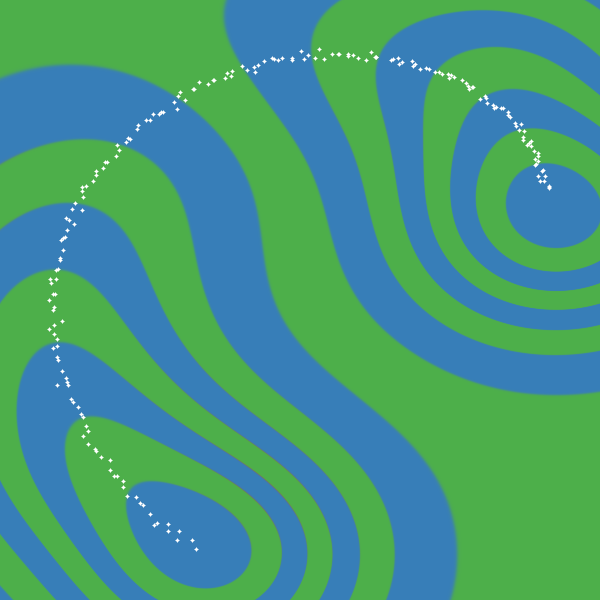
\includegraphics[width=0.45\columnwidth]{\deeplimitsfiguresdir/hidden_good} &
\begin{tikzpicture}[pile/.style={thick, ->, >=stealth'}]
    \node[anchor=south west,inner sep=0] at (0,0) {
    	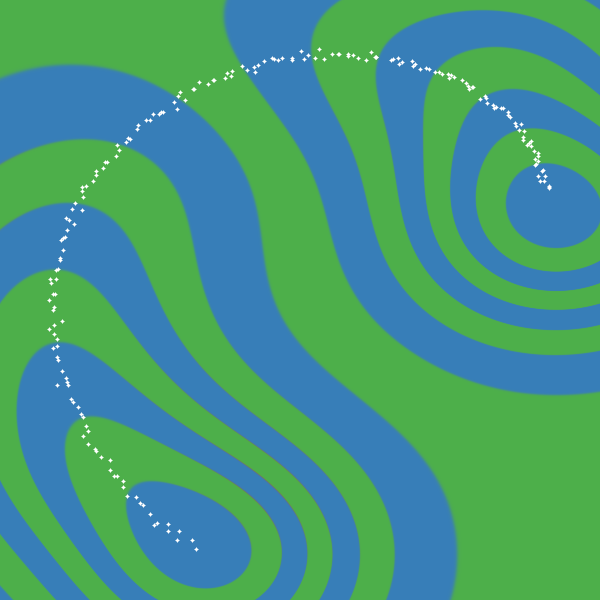
\includegraphics[clip, trim = 0cm 12cm 0cm 0.0cm, width=0.6\columnwidth]{\deeplimitsfiguresdir/hidden_good}
    };
    \coordinate (D) at (1.6,1.5);
    \coordinate (Do) at (2.5, 0.8);
    \coordinate (Dt) at (3,3);
    
    \draw[pile] (D) -- (Dt) node[above, text width=5em] { tangent };
    \draw[pile] (D) -- (Do) node[right, text width=5em] { orthogonal };
\end{tikzpicture}
%A noise-tolerant representation  of \\ a one-dimensional manifold (white)
%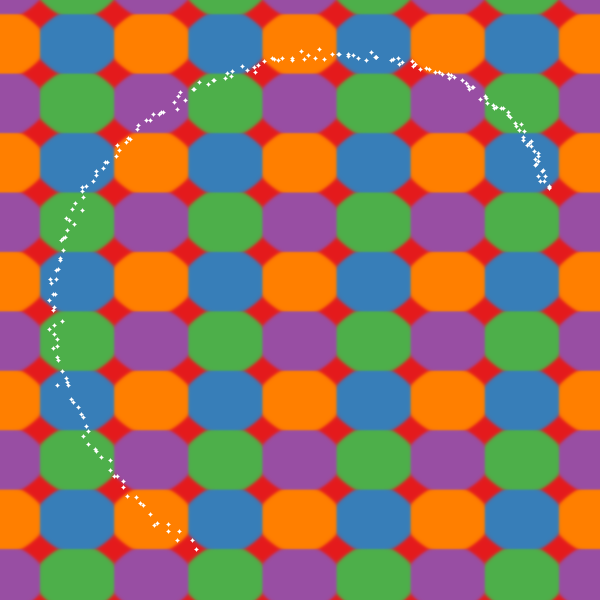
\includegraphics[clip, trim = 0cm 12cm 0cm 0.0cm, width=0.9\columnwidth]{\deeplimitsfiguresdir/hidden_bad} \\
%b) A na\"{i}ve representation (colors) \\ of a one-dimensional manifold (white)
%\end{tabular}
\caption[Desirable properties of representations of manifolds]
{Representing a 1-D data manifold.
%A representation is a function mapping the input space to some set of outputs.
Colors are a function of the computed representation of the input space.
The representation (blue \& green) changes little in directions orthogonal to the manifold (white), making it robust to noise in those directions.
The representation also varies in directions tangent to the data manifold, preserving information for later layers. 

%, and reducing the number of parameters needed to represent a datapoint.
%Representation b) changes in all directions, preserving potentially useless information.}% The representation on the right might be useful if the data were spread out in over plane.
}
\label{fig:hidden}
\end{figure}

As in \citet{rifai2011contractive}, we characterize the representational properties of a function by the singular value spectrum of the Jacobian.
The number of relatively large singular values of the Jacobian indicate the number of directions in data-space in which the representation varies significantly.
%
\newcommand{\spectrumpic}[1]{
\includegraphics[trim=4mm 1mm 4mm 2.5mm, clip, width=0.475\columnwidth]{\deeplimitsfiguresdir/spectrum/layer-#1}}%
\begin{figure}
\centering
\begin{tabular}{ccc}
& 2 Layers & 6 Layers \\
\begin{sideways} { \quad Normalized singular value} \end{sideways} & \hspace{-0.2in} \spectrumpic{2} & \hspace{-0.1in} \spectrumpic{6} \\
 & { Singular value index} & { Singular value index}
\end{tabular}
\caption[Distribution of singular values of the Jacobian of a deep \sgp{}]
{%The normalized singular value spectrum of the Jacobian of a deep \gp{} warping $\Reals^5 \to \Reals^5$.
The distribution of normalized singular values of the Jacobian of a function drawn from a 5-dimensional deep \gp{} prior 25 layers deep~(\emph{Left}) and 50 layers deep~(\emph{Right}).
As nets get deeper, the largest singular value tends to become much larger than the others.
This implies that with high probability, these functions vary little in all directions but one, making them unsuitable for computing representations of manifolds of more than one dimension.
%As depth increases, the distribution on singular values also becomes heavy-tailed.
}
\label{fig:deep_spectrum}
\end{figure}%
%
\begin{figure}%
\centering
\begin{tabular}{cc}
No transformation: $p(\vx)$ & 1 Layer: $p \left( \vf^{(1)}(\vx) \right)$ \\
\gpdrawbox{1} & \gpdrawbox{2} \\
4 Layers: $p \left( \vf^{(1:4)}(\vx) \right)$ & 6 Layers: $p \left( \vf^{(1:6)}(\vx) \right)$ \\
\gpdrawbox{4} & \gpdrawbox{6}
\end{tabular}
\caption[Points warped by a draw from a deep \sgp{}]
{Points warped by a function drawn from a deep \gp{} prior.
\emph{Top left:} Points drawn from a 2-dimensional Gaussian distribution, color-coded by their location.
\emph{Subsequent panels:} Those same points, successively warped by compositions of functions drawn from a \gp{} prior.
As the number of layers increases, the density concentrates along one-dimensional filaments.
Warpings using random finite neural networks exhibit the same pathology, but also tend to concentrate density into 0-dimensional manifolds (points) due to saturation of all of the hidden units.}
\label{fig:filamentation}
\end{figure}%
%
\Cref{fig:deep_spectrum} shows the distribution of the singular value spectrum of draws from 5-dimensional deep \gp{}s of different depths.\footnote{\citet{rifai2011contractive} analyzed the Jacobian at location of the training points, but because the priors we are examining are stationary, the distribution of the Jacobian is identical everywhere.}
As the nets gets deeper, the largest singular value tends to dominate, implying there is usually only one effective degree of freedom in the representations being computed.

\Cref{fig:filamentation} demonstrates a related pathology that arises when composing functions to produce a deep density model.
The density in the observed space eventually becomes locally concentrated onto one-dimensional manifolds, or \emph{filaments}.
This again suggests that, when the width of the network is relatively small, deep compositions of independent functions are unsuitable for modeling manifolds whose underlying dimensionality is greater than one.

%for file in `ls`; do convert $file $file; done
\newcommand{\mappic}[1]{ \includegraphics[width=0.475\columnwidth]{\deeplimitsfiguresdir/map/latent_coord_map_layer_#1} } 
\newcommand{\mappiccon}[1]{ \includegraphics[width=0.475\columnwidth]{\deeplimitsfiguresdir/map_connected/latent_coord_map_layer_#1} }
\begin{figure}
\centering
\begin{tabular}{cc}
\hspace{-0.15in} Identity Map: $\vy = \vx$ &
\hspace{-0.15in} 1 Layer: $\vy = \vf^{(1)}(\vx)$ \\
\hspace{-0.15in} \mappic{0} & \mappic{1} \\
\hspace{-0.15in} 10 Layers: $\vy = \vf^{(1:10)}(\vx)$ &
\hspace{-0.15in} 40 Layers: $\vy = \vf^{(1:40)}(\vx)$ \\
\hspace{-0.15in} \mappic{10} & \mappic{40}
\end{tabular}
\caption[Visualization of a feature map drawn from a deep \sgp{}]
{A visualization of the feature map implied by a function $\vf$ drawn from a deep \gp{}.
Colors are a function of the 2D representation $\vy = \vf(\vx)$ that each point is mapped to. % by the deep function. %that each point is mapped to after being warped by a deep \gp{}.
The number of directions in which the color changes rapidly corresponds to the number of large singular values in the Jacobian.
Just as the densities in \cref{fig:filamentation} became locally one-dimensional, there is usually only one direction that one can move $\vx$ in locally to change $\vy$.
This means that $\vf$ is unlikely to be a suitable representation for decision tasks that depend on more than one aspect of $\vx$.  Also note that the overall shape of the mapping remains the same as the number of layers increase.
For example, a roughly circular shape remains in the top-left corner even after 40 independent warpings.}
\label{fig:deep_map}
\end{figure}
%
To visualize this pathology in another way, \cref{fig:deep_map} illustrates a color-coding of the representation computed by a deep \gp{}, evaluated at each point in the input space.
After 10 layers, we can see that locally, there is usually only one direction that one can move in $\vx$-space in order to change the value of the computed representation, or to cross a decision boundary.
This means that such representations are likely to be unsuitable for decision tasks that depend on more than one property of the input.

To what extent are these pathologies present in the types of neural networks commonly used in practice?
In simulations, we found that for deep functions with a fixed hidden dimension $D$, the singular value spectrum remained relatively flat for hundreds of layers as long as $D > 100$.
Thus, these pathologies are unlikely to severely effect the relatively shallow, wide networks most commonly used in practice.





\section{Fixing the pathology}
\label{sec:fix}

As suggested by \citet[chapter 2]{neal1995bayesian}, we can fix the pathologies exhibited in figures \cref{fig:filamentation} and \ref{fig:deep_map} by simply making each layer depend not only on the output of the previous layer, but also on the original input $\vx$.  
We refer to these models as \emph{input-connected} networks, and denote deep functions having this architecture with the subscript $C$, as in $f_C(\vx)$.
Formally, this functional dependence can be written as
\begin{align}
\vf_C^{(1:L)}(\vx) = \vf^{(L)} \left( \vf_C^{(1:L-1)}(\vx), \vx \right), \quad \forall L
\end{align}
%
\Cref{fig:input-connected} shows a graphical representation of the two connectivity architectures.

\begin{figure}[h]%
\def\nodeseptwo{1.9cm}%
\def\nodesize{.35cm}%
\def\numhiddentwo{3}%
\centering
\begin{tabular}{ccc}
a) Standard \MLP{} connectivity & &
b) Input-connected architecture\\
\hspace{-4mm}
\begin{tikzpicture}[draw=black!80]
    \tikzstyle{neuron}=[circle,minimum size=17pt, draw = black!80, fill = white, thick]
    \tikzstyle{input neuron}=[neuron, fill=green!50];
    \tikzstyle{output neuron}=[neuron, fill=red!50];
    \tikzstyle{hidden neuron}=[neuron, fill=blue!50];
    \tikzstyle{pile} =[thick, ->, >=stealth', shorten <=7pt, shorten >=8pt];

    % Define the input layer node
    \coordinate (I) at (0, 0);

    % Define the hidden layer nodes
    \foreach \name / \y in {1,...,\numhiddentwo} {
        \coordinate (H-\name) at (\nodeseptwo*\y, 0);
    }

    \path[pile] (I) edge (H-1) {};
    % Connect every node            
    \foreach \name in {2,...,\numhiddentwo} {
	 	\pgfmathsetmacro\hindex{\name - 1}
		\path[pile] (H-\hindex) edge (H-\name) {};
    }

    \draw (I) node[neuron] {};
    \draw (I) node[below = 0.5cm]  {$\vx$};

    % Draw the hidden layer nodes
    \foreach \name / \y in {1,...,\numhiddentwo} {
		\draw (H-\name) node[neuron]  {};
        \draw (H-\name) node[below = 0.34cm] {$\vf^{(\y)}(\vx)$};
    }
\end{tikzpicture} &
\hspace{0.5cm} &
\begin{tikzpicture}[draw=black!80]
    \tikzstyle{neuron}=[circle,minimum size=17pt, draw = black!80, fill = white, thick]
    \tikzstyle{input neuron}=[neuron, fill=green!50];
    \tikzstyle{output neuron}=[neuron, fill=red!50];
    \tikzstyle{hidden neuron}=[neuron, fill=blue!50];
    \tikzstyle{pile} =[thick, ->, >=stealth', shorten <=7pt, shorten >=8pt];

    % Define the input layer node
    \coordinate (I) at (0, 0);

    % Define the hidden layer nodes
    \foreach \name / \y in {1,...,\numhiddentwo} {
        \coordinate (H-\name) at (\nodeseptwo*\y, 0);
    }

    % Connect every node            
    \path[pile] (I) edge (H-1) {};
    \foreach \name in {2,...,\numhiddentwo} {
		\pgfmathsetmacro\hindex{\name - 1}
		\path[pile] (H-\hindex) edge (H-\name) {};
        \path[pile] (I) edge [bend left] (H-\name) {};
    }

    \draw (I) node[neuron] {};
    \draw (I) node[below = 0.5cm]  {$\vx$};

    % Draw the hidden layer nodes
    \foreach \name / \y in {1,...,\numhiddentwo} {
		\draw (H-\name) node[neuron]  {};
       	\draw (H-\name) node[below = 0.34cm] {$\vf_C^{(\y)}(\vx)$};
    }
\end{tikzpicture}
\end{tabular}
\caption[Two different architectures for deep neural networks]
{Two different architectures for deep neural networks.
\emph{Left:} The standard architecture connects each layer's outputs to the next layer's inputs.
\emph{Right:} The input-connected architecture also connects the original input $\vx$ to each layer.}
\label{fig:input-connected}
\end{figure}%

Similar connections between non-adjacent layers can also be found the primate visual cortex \citep{maunsell1983connections}.
Visualizations of the resulting prior on functions are shown in \cref{fig:deep_draw_1d_connected,fig:no_filamentation,fig:deep_map_connected}.


\begin{figure}[h]
\centering
\setlength{\tabcolsep}{1.5pt}
\begin{tabular}{ccccc}
& 1 Layer & 2 Layers & 5 Layers & 10 Layers \\
\raisebox{0.6cm}{\rotatebox{90}{$f_C^{(1:L)}(x)$}} &
\onedsamplepiccon{1} &
\onedsamplepiccon{2} &
\onedsamplepiccon{5} &
\onedsamplepiccon{10} \\[-3pt]
 & $x$ & $x$ & $x$ & $x$
\end{tabular}
\caption[A draw from a 1D deep \sgp{} prior with each layer connected to the input]
{A draw from a 1D deep \gp{} prior having each layer also connected to the input.
The $x$-axis is the same for all plots.
Even after many layers, the functions remain relatively smooth in some regions, while varying rapidly in other regions.
Compare to standard-connectivity deep \gp{} draws shown in \cref{fig:deep_draw_1d}.}
\label{fig:deep_draw_1d_connected}
\end{figure}
%
\newcommand{\gpdrawboxcon}[1]{
\setlength\fboxsep{0pt}
\hspace{-0.2in} 
\fbox{
\includegraphics[width=0.464\columnwidth]{\deeplimitsfiguresdir/deep_draws_connected/deep_sample_connected_layer#1}
}}
%
\begin{figure}
\centering
\begin{tabular}{cc}
3 Connected layers: $p \left( \vf_C^{(1:3)}(\vx) \right)$ & 6 Connected layers: $p \left( \vf_C^{(1:6)}(\vx) \right)$ \\
\gpdrawboxcon{3} &
\gpdrawboxcon{6}
\end{tabular}
\caption[Points warped by a draw from an input-connected deep \sgp{}]
{Points warped by a draw from a deep \sgp{} with each layer connected to the input $\vx$.
%\emph{Top left:} Points drawn from a 2-dimensional Gaussian distribution, color-coded by their location.
%\emph{Subsequent panels:} Those same points, successively warped by functions drawn from a \gp{} prior.
As depth increases, the density becomes more complex without concentrating only along one-dimensional filaments.}
\label{fig:no_filamentation}
\end{figure}
%
\begin{figure}
\centering
\newcommand{\spectrumpiccon}[1]{
\includegraphics[trim=4mm 1mm 4mm 2.5mm, clip, width=0.475\columnwidth]{\deeplimitsfiguresdir/spectrum/con-layer-#1}} 
\begin{tabular}{ccc}
 & 25 layers &  50 layers \\
\hspace{-0.5cm} \begin{sideways} {\quad Normalized singular value} \end{sideways} & \hspace{-0.2in} \spectrumpiccon{25} & \hspace{-0.16in} \spectrumpiccon{50} \\
 & {Singular value number} & {Singular value number}
\end{tabular}
\caption[Distribution of singular values of an input-connected deep \sgp{}]
{The distribution of singular values drawn from 5-dimensional input-connected deep \gp{} priors, 25 layers deep (\emph{Left}) and 50 layers deep (\emph{Right}).
Compared to the standard architecture, the singular values are more likely to remain the same size as one another, meaning that the model outputs are more often sensitive to several directions of variation in the input.}
\label{fig:good_spectrum}
\end{figure}
%
%
\begin{figure}
\centering
\begin{tabular}{cc}
\hspace{-0.15in} Identity map: $\vy = \vx$ &
\hspace{-0.15in} 2 Connected layers: $\vy = \vf^{(1:2)}(\vx)$ \\
\hspace{-0.15in} \mappic{0} & \mappiccon{2} \\
\hspace{-0.15in} 10 Connected layers: $\vy = \vf^{(1:10)}(\vx)$ &
\hspace{-0.15in} 20 Connected layers: $\vy = \vf^{(1:20)}(\vx)$ \\
\hspace{-0.15in} \mappiccon{10} & \mappiccon{20}
\end{tabular}
\caption[Feature map of an input-connected deep \sgp{}]
{The feature map implied by a function $\vf$ drawn from a deep \gp{} prior with each layer also connected to the input $\vx$, visualized at various depths.
Compare to the map shown in \cref{fig:deep_map}.
%Just as the densities in \cref{fig:no_filamentation} remained locally two-dimensional even after many warpings, 
In the mapping shown here there are sometimes two directions that one can move locally in $\vx$ to in order to change the value of $\vf(\vx)$.
This means that the input-connected prior puts significant probability mass on a greater variety of types of representations, some of which depend on all aspects of the input.
}
\label{fig:deep_map_connected}
\end{figure}


The Jacobian of an input-connected deep function is defined by the recurrence
%
\newcommand{\sbi}[2]{\left[ \! \begin{array}{c} #1 \\ #2 \end{array} \! \right]} 
%\newcommand{\sbi}[2]{\left[ #1 \quad \!\! #2 \right]} 
\begin{align}
{J_C^{(1:L)} = J^{(L)} \sbi{ J_C^{(1:L-1)}}{I_D}}.
\end{align}
%
%So the entire Jacobian has the form:
%
%\begin{align}
%J^{1:L}(x) = J^L \sbi{ J^{L-1} \sbi{ \dots J^{4} \sbi{ J^{3} \sbi{ J^2 J^1 }{ I_D }}{ I_D } \dots }{ I_D \\ %\vdots }}{ I_D}
%\end{align}
%
where $I_D$ is a $D$-dimensional identity matrix.
Thus the Jacobian of an input-connected deep \gp{} is a product of independent Gaussian matrices each with an identity matrix appended.
\Cref{fig:good_spectrum} shows that with this architecture, even 50-layer deep \gp{}s have well-behaved singular value spectra.

The pathology examined in this section is an example of the sort of analysis made possible by a well-defined prior on functions.
%As explained in \cref{sec:relating}, \gp{}s are examples of a particular limit of Bayesian neural networks.
The figures and analysis done in this section could be done using Bayesian neural networks with finite numbers of nodes, but would be more difficult.
In particular, care would need to be taken to ensure that the networks do not produce degenerate mappings due to saturation of the hidden units.





\section{Deep kernels}
\label{sec:deep_kernels}

\cite{ bengio2006curse} showed that kernel machines have limited generalization ability when they use ``local'' kernels such as the squared-exp.
However, as shown in \cref{ch:kernels,ch:grammar,ch:additive}, structured, non-local kernels can 
%be constructed through addition and multiplication which 
allow extrapolation.
Another way to build non-local kernels is by composing fixed feature maps, creating \emph{deep kernels}.
To return to an example given in \cref{sec:expressing-symmetries}, periodic kernels can be viewed as a 2-layer-deep kernel, in which the first layer maps $x \rightarrow [\sin(x), \cos(x)]$, and the second layer maps through basis functions corresponding to the implicitly feature map giving rise to an \kSE{} kernel.

This section builds on the work of \citet{cho2009kernel}, who derived several kinds of deep kernels by composing multiple layers of feature mappings.

%In addition to analyzing \MLP{}s with random weights, we can also analyze fixed feature mappings with different connectivity architectures.
 
%We can construct other useful kernels by composing fixed feature maps several times, creating deep kernels.


%Given a kernel $k_1(\vx, \vx') = \hPhi(\vx) \tra \hPhi(\vx')$, 
In principle, one can compose the implicit feature maps of any two kernels $k_a$ and $k_b$ to get a new kernel, which we denote by $\left( k_b \circ k_a \right)$:
%
\begin{align}
k_a(\vx, \vx') & = \hPhi_a(\vx) \tra \hPhi_a(\vx') \\
k_b(\vx, \vx') & = \hPhi_b(\vx) \tra \hPhi_b(\vx') \\
\left( k_b \circ k_a \right)(\vx, \vx') & = k_b \big(\hPhi_a(\vx), \hPhi_a(\vx') \big) 
 = \left[ \hPhi_b \left( \hPhi_a(\vx) \right)\right] \tra \hPhi_b \left(\hPhi_a(\vx') \right)
\end{align}
%
However, this composition might not always have a closed form if the number of hidden features of either kernel is infinite.

Fortunately, composing the squared-exp (\kSE{}) kernel with the implicit mapping given by any other kernel has a simple closed form.
If $k(\vx, \vx') = \hPhi(\vx)\tra \hPhi(\vx')$, then
%, this composition operation has a closed form for any starting kernel:% for any set of starting features $\hPhi_n(\vx)$:
%
\begin{align}
%k_1(\vx, \vx') & = \exp \left( -\frac{1}{2} ||\vx - \vx'||_2^2 \right) \\
\left( \kSE \circ k \right) \left( \vx, \vx' \right) & = k_{SE} \big( \hPhi(\vx), \hPhi(\vx') \big) \\
%& = \left( \hPhi^{SE} \left(\hPhi^{1}(\vx) \right) \right) \tra \hPhi^{SE} \left( \hPhi^{1}(\vx') \right) \\
& = \exp \left( -\frac{1}{2} || \hPhi(\vx) - \hPhi(\vx')||_2^2 \right) \\
%k_{n+1}(\vx, \vx') 
%& = \exp \left( -\frac{1}{2} \sum_i \left[ \hphi_n^{(i)}(\vx) - \hphi_n^{(i)}(\vx') \right]^2 \right) \\
& = \exp\left ( -\frac{1}{2} \left[ \hPhi(\vx) \tra \hPhi(\vx) - 2 \hPhi(\vx) \tra \hPhi(\vx') + \hPhi(\vx') \tra \hPhi(\vx') \right] \right)  \\
%k_2(\vx, \vx') & = \exp \left( -\frac{1}{2} \left[ \sum_i \hphi_i(\vx)^2 - 2 \sum_i \hphi_i(\vx) \hphi_i(\vx') + \sum_i \hphi_i(\vx')^2 \right] \right) \\
%k_{n+1}(\vx, \vx') 
& = \exp \left( -\frac{1}{2} \big[ k(\vx, \vx) - 2 k(\vx, \vx') + k(\vx', \vx') \big] \right) \; .
%k_{n+1}(\vx, \vx') 
%& = \exp \left( k_1(\vx, \vx') - 1 \right) \qquad \textnormal{(if $k_1(\vx, \vx) = 1$)} \nonumber
\end{align}
%
%\begin{figure}
%\centering
%\begin{tabular}{ccc}
%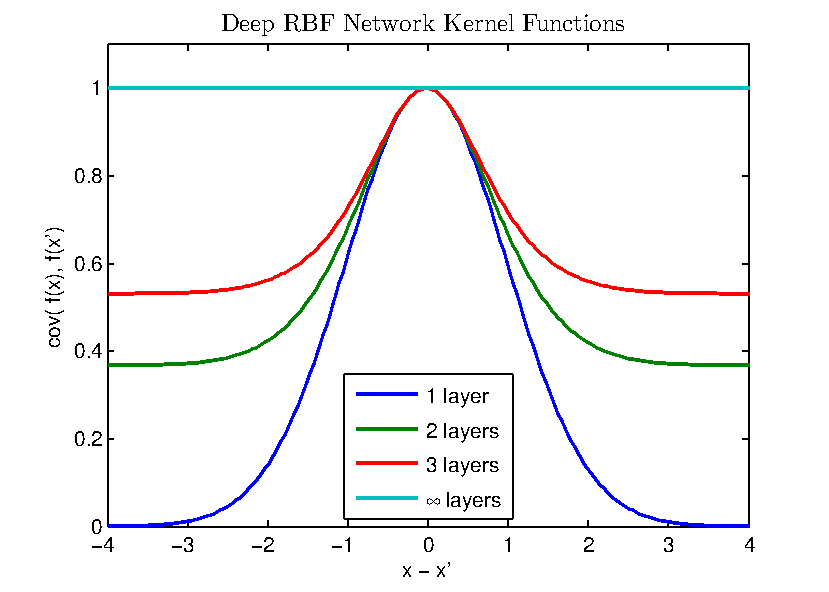
\includegraphics[width=0.5\columnwidth, clip, trim = 0cm 0cm 0cm 0.61cm]{\deeplimitsfiguresdir/deep_kernel} &
%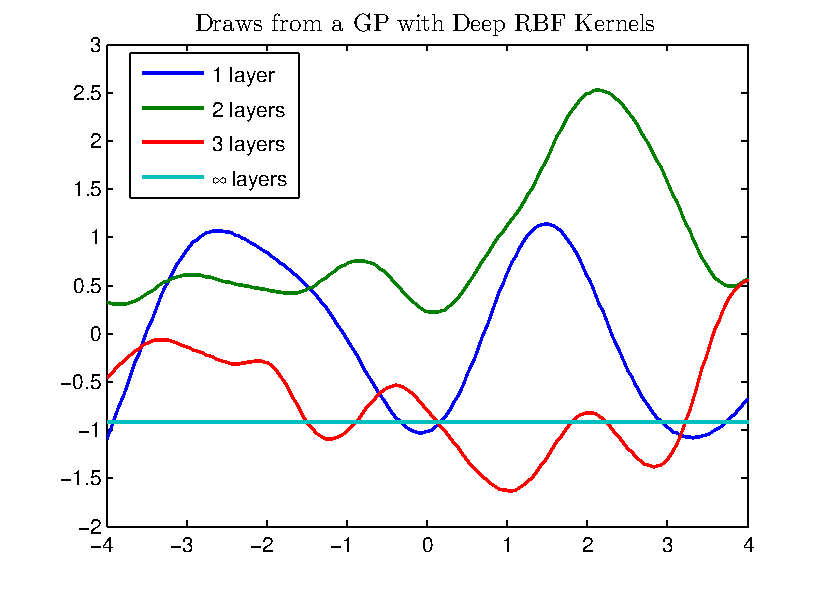
\includegraphics[width=0.5\columnwidth, clip, trim = 0cm 0cm 0cm 0.61cm]{\deeplimitsfiguresdir/deep_kernel_draws} \\
%Kernel derived from iterated feature transforms & Draws from the corresponding kernel
%\end{tabular}
%\caption{A degenerate kernel produced by repeatedly applying a feature transform.}
%\label{fig:deep_kernel}
%\end{figure}
%
%Thus, if $k_1(x,y) = e^{-||x - y||2}$, then the two-layer kernel is simply $k_2(x,y) = e^{k_1(x, y) - 1}$.  This formula is true for every layer: $k_{n+1}(x,y) = e^{k_n(x, y) - 1}$.
%
%Note that nothing in this derivation depends on details of $k_n$, except that $k_n( \vx, \vx) = 1$.
%Note that this result holds for any base kernel $k_n$, as long as $k_n( \vx, \vx) = 1$.
%  Because this is true for $k_2$ as well, this recursion holds in general, and we have that $k_{n+1}(x,y) = e^{k_n(x, y) - 1}$.  
This formula expresses the composed kernel $(\kSE \circ k)$ exactly in terms of evaluations of the original kernel $k$.

\subsection{Infinitely deep kernels}
What happens when one repeatedly composes feature maps many times, starting with the squared-exp kernel?
If the output variance of the \kSE{} is normalized to ${k(\vx,\vx) = 1}$, then the infinite limit of composition with \kSE{} converges to ${\left(\kSE \circ \kSE \circ \ldots \circ \kSE\right)(\vx,\vx') = 1}$ for all pairs of inputs.
A constant covariance corresponds to a prior on constant functions ${f(\vx) = c}$.

%Figure \ref{fig:deep_kernel_connected} shows this kernel at different depths, including the degenerate limit.  
%
%One interpretation of why repeated feature transforms lead to this degenerate prior is that each layer can only lose information about the previous set of features.  
%In the limit, the transformed features contain no information about the original input $\vx$.  Since the function doesn't depend on its input, it must be the same everywhere.

%\subsubsection{A non-degenerate construction}

As above, we can overcome this degeneracy by connecting the input $\vx$ to each layer.
To do so, we concatenate the composed feature vector at each layer, $\hPhi^{(1:\ell)}(\vx)$, with the input vector $\vx$ to produce an input-connected deep kernel $k_C^{(1:L)}$, defined by:
%
\begin{align}
%k_1(\vx, \vx') & = \exp \left( -\frac{1}{2} ||\vx - \vx'||_2^2 \right) \\
k_C^{(1:\ell + 1)}(\vx, \vx')
& = \exp \left( -\frac{1}{2} \left|\left| 
\left[ \! \begin{array}{c} \hPhi^{(1:\ell)}(\vx) \\ \vx \end{array} \! \right] - 
\left[ \! \begin{array}{c} \hPhi^{(1:\ell)}(\vx') \\ \vx' \end{array} \! \right] \right| \right|_2^2 \right) \\
%k_{n+1}(\vx, \vx') 
%& = \exp \left( -\frac{1}{2} \sum_i \left[ \hphi_i(\vx) - \hphi_i(\vx') \right]^2 -\frac{1}{2} || \vx - \vx' ||_2^2 \right) \\
%k_{n+1}(\vx, \vx') & = \exp\left ( -\frac{1}{2} \sum_i \left[ \hphi_i(\vx)^2 - 2 \hphi_i(\vx) \hphi_i(\vx') + \hphi_i(\vx')^2 \right]  -\frac{1}{2} || \vx - \vx' ||_2^2 \right) \\
%k_2(\vx, \vx') & = \exp \left( -\frac{1}{2} \left[ \sum_i \hphi_i(\vx)^2 - 2 \sum_i \hphi_i(\vx) \hphi_i(\vx') + \sum_i \hphi_i(\vx')^2 \right] \right) \\
%k_2(\vx, \vx') & = \exp \left( -\frac{1}{2} \left[ k_1(\vx, \vx) - 2 k_1(\vx, \vx') + k_1(\vx', \vx') \right] \right) \\
%k_{n+1}(\vx, \vx') 
%& = \exp \left( k_n(\vx, \vx') - 1 -\frac{1}{2} || \vx - \vx' ||_2^2 \right)
& = \exp \Big( -\frac{1}{2} \big[ k_C^{(1:\ell)}(\vx, \vx) - 2 k_C^{(1:\ell)}(\vx, \vx') 
 + k_C^{(1:\ell)}(\vx', \vx') {\color{black} - || \vx - \vx' ||_2^2} \big] \Big) \nonumber
\end{align}
%
Starting with the squared-exp kernel, this repeated mapping satisfies
\begin{align}
k_C^{(1:\infty)}(\vx, \vx') - \log \left( k_C^{(1:\infty)}(\vx, \vx') \right) = 1 + \frac{1}{2} || \vx - \vx' ||_2^2 \,.
\end{align}
%
\begin{figure}
\centering
\begin{tabular}{cc}
Input-connected deep kernels & Draws from corresponding \gp{}s \\
\hspace{-0.3cm}
\rotatebox{90}{$\qquad \qquad k(x, x')$}
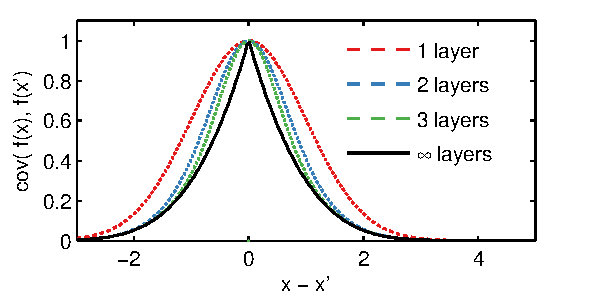
\includegraphics[width=0.465\columnwidth, clip, trim = 1.3cm 0.4cm 0.9cm 0.3cm]{\deeplimitsfiguresdir/deep_kernel_connected} &
\hspace{-0.3cm}
\rotatebox{90}{$\qquad \qquad f(x)$}
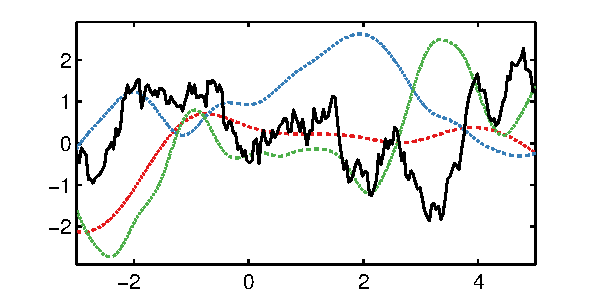
\includegraphics[width=0.44\columnwidth, clip, trim = 1.29cm 0.1cm 0.9cm 0.35cm]{\deeplimitsfiguresdir/deep_kernel_connected_draws} \\
$x - x'$ &  $x$
\end{tabular}
\caption[Infinitely deep kernels]{
\emph{Left:} Input-connected deep kernels of different depths.
By connecting the input $\vx$ to each layer, the kernel can still depend on its input even after arbitrarily many layers of composition.
\emph{Right:} Draws from \gp{}s with deep input-connected kernels.}
\label{fig:deep_kernel_connected}
\end{figure}
%
The solution to this recurrence is related to the Lambert W function~\citep{corless1996lambertw} and has no closed form.
In one input dimension, it has a similar shape to the Ornstein-Uhlenbeck covariance ${\OU(x,x') = \exp( -|x - x'| )}$ but with lighter tails.
Samples from a \gp{} prior having this kernel are not differentiable, and are locally fractal.
\Cref{fig:deep_kernel_connected} shows this kernel at different depths, as well as samples from the corresponding \gp{} priors.
%\item This kernel has smaller correlation than the squared-exp everywhere except at $\vx = \vx'$.  
%\item The tails have the same form as the squared-exp.

One can also consider two related connectivity architectures: one in which each layer is connected to the output layer, and another in which every layer is connected to all subsequent layers.
It is easy to show that in the limit of infinite depth of composing \kSE{} kernels, both these architectures converge to $k(\vx, \vx') = \delta( \vx, \vx' )$, the white noise kernel.



%\subsection{A fully-connected kernel}
%However, connecting every layer to every subsequent layer leades to a pathology:
%\begin{align}
%k_1(\vx, \vx') & = \exp \left( -\frac{1}{2} ||\vx - \vx'||_2^2 \right) \\
%k_{n+1}(\vx, \vx') & = \exp \left( -\frac{1}{2} \left|\left| \left[ \! \begin{array}{c} \hPhi_n(\vx) \\ \hPhi_{n-1}(\vx') \end{array} \! \right]  - \left[ \! \begin{array}{c} \hPhi_n(\vx') \\ \hPhi_{n-1}(\vx') \end{array} \! \right] \right| \right|_2^2 \right) \\
%k_{n+1}(\vx, \vx') & = \exp \left( -\frac{1}{2} \sum_i \left[ \hphi^{(i)}_n(\vx) - \hphi^{(i)}_n(\vx') \right]^2 -\frac{1}{2} \sum_i \left[ \hphi^{(i)}_{n-1}(\vx) - \hphi^{(i)}_{n-1}(\vx') \right]^2 \right)\\
%k_{n+1}(\vx, \vx') & = \exp\left ( -\frac{1}{2} \sum_i \left[ \hphi_i(\vx)^2 - 2 \hphi_i(\vx) \hphi_i(\vx') + \hphi_i(\vx')^2 \right]  -\frac{1}{2} || \vx - \vx' ||_2^2 \right) \\
%k_2(\vx, \vx') & = \exp \left( -\frac{1}{2} \left[ \sum_i \hphi_i(\vx)^2 - 2 \sum_i \hphi_i(\vx) \hphi_i(\vx') + \sum_i \hphi_i(\vx')^2 \right] \right) \\
%k_2(\vx, \vx') & = \exp \left( -\frac{1}{2} \left[ k_1(\vx, \vx) - 2 k_1(\vx, \vx') + k_1(\vx', \vx') \right] \right) \\
%k_{n+1}(\vx, \vx') & = \exp \left( k_n(\vx, \vx') - 1 \right) \exp \left( k_{n-1}(\vx, \vx') - 1 \right)
%k_{n+1}(\vx, \vx') & = \prod_{i=1}^n \prod_{j=1}^i \exp \left( k_i(\vx, \vx') - 1 \right)
%\end{align}
%Which has the solution $k_\infty = \delta( \vx = \vx' )$, a white noise kernel.


%\subsection{Connecting every layer to the end}
%There is a fourth possibilty (suggested by Carl), of connecting every layer to the output:
%\begin{align}
%k_n(\vx, \vx') & = \exp \left( -\frac{1}{2} || \hPhi_n(\vx) - \hPhi_n(\vx')||_2^2 \right) \\
%k_{n+1}(\vx, \vx') & = \exp \left( k_n(\vx, \vx') - 1 \right) \\
%k_{L}(\vx, \vx') & = \prod_{i=1}^L \exp \left( k_i(\vx, \vx') - 1 \right)
%\end{align}
%Which also has the solution $k_\infty = \delta( \vx = \vx' )$, a white noise kernel.


\subsection{When are deep kernels useful models?}

Kernels correspond to fixed feature maps, and so kernel learning is an example of implicit representation learning. %can compute %useful representations.
As we saw in \cref{ch:kernels,ch:grammar}, kernels can capture rich structure and can enable many types of generalization.
 %, such as affine invariance in images \citep{kondor2008group}.
%\cite{salakhutdinov2008using} used a deep neural network to learn feature transforms for kernels, which learn invariants in an unsupervised manner.
We believe that the relatively uninteresting properties of the deep kernels derived in this section simply reflect the fact that an arbitrary computation, even if it is ``deep'', is not likely to give rise to a useful representation unless combined with learning.
To put it another way, any fixed representation is unlikely to be useful unless it has been chosen specifically for the problem at hand.






\section{Related work}

\subsubsection{Deep Gaussian processes}
\citet[chapter 2]{neal1995bayesian} explored properties of arbitrarily deep Bayesian neural networks, including those that would give rise to deep \gp{}s.
He noted that infinitely deep random neural networks without extra connections to the input would be equivalent to a Markov chain, and therefore would lead to degenerate priors on functions.
He also suggested connecting the input to each layer in order to fix this problem.
Much of the analysis in this chapter can be seen as a more detailed investigation, and vindication, of these claims.

The first instance of deep \gp{}s being used in practice was \citep{lawrence2007hierarchical}, who presented a model called ``hierarchical \gplvm{}s'', in which time was mapped through a composition of multiple \gp{}s to produce observations.

%The term ``deep Gaussian processes'' first appeared in \citet{damianou2012deep}, where it referred to a latent variable model whose warping function was defined by a composition of \gp{}s.
The term ``deep Gaussian processes'' was first used by \citet{damianou2012deep}, who developed a variational inference method, analyzed the effect of automatic relevance determination, and showed that deep \gp{}S could learn with relatively little data.
%I propose that this model might be more clearly described as a ``deep \gplvm{}'', and that the term ``deep Gaussian process'' should be reserved for describing compositions of functions drawn from \gp{} priors.
%
They used the term ``deep \gp{}'' to refer both to supervised models (compositions of \gp{}s) and to unsupervised models (compositions of \gplvm{}s).
This conflation may be reasonable, since the activations of the hidden layers are themselves latent variables, even in supervised settings:
Depending on kernel parameters, each latent variable may or may not depend on the layer below.

In general, supervised models can also be latent-variable models.
For example, \citet{wang2012gaussian} investigated single-layer \gp{} regression models that had additional latent inputs.

\subsubsection{Nonparametric neural networks}
%Other Bayesian deep neural network models have been proposed by, for example, . % and Sum-product networks \cite{poon2011sum}  
\citet{adams2010learning} proposed a prior on arbitrarily deep Bayesian networks having an unknown and unbounded number of parametric hidden units in each layer.
Their architecture has connections only between adjacent layers, and so may have similar pathologies to the one discussed in the chapter as the number of layers increases.

\citet{wilson2012gaussian} introduced Gaussian process regression networks, which are defined as a matrix product of draws from \gp{}s priors, rather than a composition.
These networks have the form:
%The form of a \gprn{} is
%
\begin{align}
\vy(\vx) & = \vW(\vx) \vf(\vx) \qquad \textnormal{where each} \; f_{d}, W_{d,j} \simiid \GPt{\vzero}{\kSE + \kWN} .
\end{align}
%
We can easily define a ``deep'' Gaussian process regression network:
%
\begin{align}
\vy(\vx) = \vW^{(3)}(\vx) \vW^{(2)}(\vx) \vW^{(1)}(\vx) \vf(\vx)
\end{align}
%
which repeatedly adds and multiplies functions drawn from \gp{}s, in contrast to deep \gp{}s, which repeatedly compose functions.
This prior on functions has a similar form to the Jacobian of a deep \gp{} (\cref{eq:jacobian-of-deep-gp}), and so might be amenable to a similar analysis to that of section \ref{sec:characterizing-deep-gps}.

%
%This model has a similar form to the Jacobian of deep \gp{}, (since each row of the Jacobian is jointly a \gp{} but with with a kernel given by \eqref{eq:deriv-kernel}) except that the Jacobian is evaluated at the output from previous layers:
%
%\begin{align}
%\vy(\vx) = J^3(\vf^2(\vx)) J^2(\vf^1(\vx)) J^1(\vx)
%\end{align}
%

\subsubsection{Information-preserving architectures}
Deep density networks \citep{rippel2013high} are constructed through a series of parametric warpings of fixed dimension, with penalty terms encouraging the preservation of information about lower layers.
This is another promising approach to fixing the pathology discussed in \cref{sec:formalizing-pathology}.

\subsubsection{Recurrent networks}
\citet{bengio1994learning} and \citet{pascanu2012understanding} analyzed a related problem with gradient-based learning in recurrent networks, the ``exploding-gradients'' problem.
They noted that in recurrent neural networks, the size of the training gradient can grow or shrink exponentially as it is back-propagated, making gradient-based training difficult.

\citet{hochreiter1997long} addressed the exploding-gradients problem by introducing hidden units designed to have stable gradients.
This architecture is known as long short-term memory.

\subsubsection{Deep kernels}

The first systematic examination of deep kernels was done by \citet{cho2009kernel}, who derived closed-form composition rules for $\kSE$, polynomial, and arc-cosine kernels, and showed that deep arc-cosine kernels performed competitively in machine-vision applications when used in a \SVM{}.
%\citet{cho2012kernel} 

\citet{hermans2012recurrent} constructed deep kernels in a time-series setting, constructing kernels corresponding to infinite-width \emph{recurrent} neural networks.
They also proposed concatenating the implicit feature vectors from previous time-steps with the current inputs, resulting in an architecture analogous to the input-connected architecture proposed by \citet[chapter 2]{neal1995bayesian}.

\subsubsection{Analyses of deep learning}
\citet{montavon2010layer} performed a layer-wise analysis of deep networks, and noted that the performance of \MLP{}s degrades as the number of layers with random weights increases, a result consistent with the analysis of this chapter.

The experiments of \citet{saxe2011random} suggested that most of the good performance of convolutional neural networks could be attributed to the architecture alone.
Later, \citet{saxedynamics} looked at the dynamics of gradient-based training methods in deep \emph{linear} networks as a tractable approximation to standard deep (nonlinear) neural networks.  




%\section{Discussion}


%\paragraph{Recursive learning method}
%Just as layer-wise unsupervised pre-training encourages the projection of the data into a representation with independent features in the higher layers, so does the procedure outlined here.  This is because the isotropic kernel does not penalize independence between different dimensions, only the number of dimensions.


\subsubsection{Source code}
Source code to produce all figures is available at \url{http://www.github.com/duvenaud/deep-limits}.
This code is also capable of producing visualizations of mappings such as \cref{fig:deep_map,fig:deep_map_connected} using neural nets instead of \gp{}s at each layer.


\section{Conclusions}

%In this work, we established a number of propositions which help us gain insight into the properties of very deep models, and allow making informed choices regarding their architecture.

This chapter demonstrated that well-defined priors allow explicit examination of the assumptions being made about functions being modeled by different neural network architectures.
As an example of the sort of analysis made possible by this approach, we attempted to gain insight into the properties of deep neural networks by characterizing the sorts of functions likely to be obtained under different choices of priors on compositions of functions.
%established a number of propositions which help us gain insight into the properties of very deep models, and allow making informed choices regarding their architecture.

%First, we identified equivalences between multi-layer perceptions and deep \gp{}s --- namely, that a deep \gp{} can be written as an \MLP{}s with a finite number of nonparametric hidden units, or as an \MLP{} with infinitely-many parametric hidden units.
First, we identified deep Gaussian processes as an easy-to-analyze model corresponding to multi-layer preceptrons having nonparametric activation functions.
%  We also showed several other connections between deep \MLP{}s and different Gaussian process models. %equivalences between multi-layer perceptions and deep \gp{}s --- namely, that a deep \gp{} can be written as an \MLP{}s with a finite number of nonparametric hidden units, or as an \MLP{} with infinitely-many parametric hidden units.
%
%Second, we characterized the derivatives and Jacobians of deep \gp{}s through products of independent Gaussian matrices. % can be characterized using random matrix theory, which we applied to establish results regarding the distribution over the Jacobian of the composition transformation. 
We then showed that representations based on repeated composition of independent functions exhibit a pathology where the representations becomes invariant to all but one direction of variation. % This leads to extremely restricted expressiveness of such deep models in the limit of increasing number of layers. 
Finally, we showed that this problem could be alleviated by connecting the input to each layer.
%proposed a way to alleviate this problem: connecting the input to each layer of a deep representation allows us to construct priors on deep functions that do not exhibit the information-capacity pathology.
%
We also examined properties of deep kernels, corresponding to arbitrarily many compositions of fixed feature maps.
%Finally, we derived models obtained by performing dropout on Gaussian processes, finding a tractable approximation to exact dropout in \gp{}s.

Much recent work on deep networks has focused on weight initialization \citep{martens2010deep}, regularization \citep{lee2007sparse} and network architecture \citep{gens2013learning}.
%However, the interactions between these different design decisions can be complex and difficult to characterize.
%We propose to approach the design of deep architectures by examining the problem of assigning priors to nested compositions of functions.
% Although inference in fully Bayesian models is generally challenging, well-defined priors allow us to encode our beliefs into models in a data-independent way. 
If we can identify priors that give our models desirable properties, these might in turn suggest regularization, initialization, and architecture choices that also provide such properties.

Existing neural network practice also requires expensive tuning of model hyperparameters such as the number of layers, the size of each layer, and regularization penalties by cross-validation.
One advantage of deep \gp{}s is that the approximate marginal likelihood allows a principled method for automatically determining such model choices.




\outbpdocument{
%This will be ignored, it's just so that Gummi can find the bibliography.
\bibliographystyle{plainnat}
\bibliography{references.bib}
qwerty
}


%%*****************************************************************************************
%*********************************** Second Chapter **************************************
%*****************************************************************************************

\chapter{My Second Chapter}

\ifpdf
    \graphicspath{{Chapter2/Figs/Raster/}{Chapter2/Figs/PDF/}{Chapter2/Figs/}}
\else
    \graphicspath{{Chapter2/Figs/Vector/}{Chapter2/Figs/}}
\fi


\section[Short title]{Reasonably Long Section Title}

% Uncomment this line, when you have siunitx package loaded.
%The SI Units for dynamic viscosity is \si{\newton\second\per\metre\squared}.
I'm going to randomly include a picture Figure~\ref{fig:minion}.


If you have trouble viewing this document contact Krishna \href{mailto:kks32@cam.ac.uk}{kks32@cam.ac.uk}. 


\begin{figure}[htbp!] 
\centering    

\includegraphics[width=1.0\textwidth]{minion}
\caption[Minion]{This is just a long figure caption for the minion in Despicable Me from Pixar}
\label{fig:minion}
\end{figure}


\section*{Enumeration}
\begin{enumerate}
\item The first topic is dull
\item The second topic is duller
\begin{enumerate}
\item The first subtopic is silly
\item The second subtopic is stupid
\end{enumerate}
\item The third topic is dullest
\end{enumerate}

\section*{itemize}
\begin{itemize}
\item The first topic is dull
\item The second topic is duller
\begin{itemize}
\item The first subtopic is silly
\item The second subtopic is stupid
\end{itemize}
\item The third topic is dullest
\end{itemize}

\section*{description}
\begin{description}
\item[The first topic] is dull
\item[The second topic] is duller
\begin{description}
\item[The first subtopic] is silly
\item[The second subtopic] is stupid
\end{description}
\item[The third topic] is dullest
\end{description}


\clearpage

\tochide\section{Hidden Section}
\textbf{Lorem ipsum dolor sit amet}, \textit{consectetur adipiscing elit}. In magna nisi, aliquam id blandit id, congue ac est. Fusce porta consequat leo. Proin feugiat at felis vel consectetur. Ut tempus ipsum sit amet congue posuere. Nulla varius rutrum quam. Donec sed purus luctus, faucibus velit id, ultrices sapien. Cras diam purus, tincidunt eget tristique ut, egestas quis nulla. Curabitur vel iaculis lectus. Nunc nulla urna, ultrices et eleifend in, accumsan ut erat. In ut ante leo. Aenean a lacinia nisl, sit amet ullamcorper dolor. Maecenas blandit, tortor ut scelerisque congue, velit diam volutpat metus, sed vestibulum eros justo ut nulla. Etiam nec ipsum non enim luctus porta in in massa. Cras arcu urna, malesuada ut tellus ut, pellentesque mollis risus.Morbi vel tortor imperdiet arcu auctor mattis sit amet eu nisi. Nulla gravida urna vel nisl egestas varius. Aliquam posuere ante quis malesuada dignissim. Mauris ultrices tristique eros, a dignissim nisl iaculis nec. Praesent dapibus tincidunt mauris nec tempor. Curabitur et consequat nisi. Quisque viverra egestas risus, ut sodales enim blandit at. Mauris quis odio nulla. Cras euismod turpis magna, in facilisis diam congue non. Mauris faucibus nisl a orci dictum, et tempus mi cursus.

Etiam elementum tristique lacus, sit amet eleifend nibh eleifend sed \footnote{My footnote goes blah blah blah! \dots}. Maecenas dapibu augue ut urna malesuada, non tempor nibh mollis. Donec sed sem sollicitudin, convallis velit aliquam, tincidunt diam. In eu venenatis lorem. Aliquam non augue porttitor tellus faucibus porta et nec ante. Proin sodales, libero vitae commodo sodales, dolor nisi cursus magna, non tincidunt ipsum nibh eget purus. Nam rutrum tincidunt arcu, tincidunt vulputate mi sagittis id. Proin et nisi nec orci tincidunt auctor et porta elit. Praesent eu dolor ac magna cursus euismod. Integer non dictum nunc.


\begin{landscape}

\section*{Subplots}
I can cite Wall-E (see Fig.~\ref{fig:WallE}) and Minions in despicable me (Fig.~\ref{fig:Minnion}) or I can cite the whole figure as Fig.~\ref{fig:animations}


\begin{figure}
  \centering
  \subfloat[A Tom and Jerry]{\label{fig:TomJerry}
\includegraphics[width=0.3\textwidth]{TomandJerry}}                
  \subfloat[A Wall-E]{\label{fig:WallE}\includegraphics[width=0.3\textwidth]{WallE}}
  \subfloat[A Minion]{\label{fig:Minnion}\includegraphics[width=0.3\textwidth]{minion}}
  \caption{Best Animations}
  \label{fig:animations}
\end{figure}


\end{landscape}

%\chapter{My Third Chapter}

% **************************** Define Graphics Path **************************
\ifpdf
    \graphicspath{{Chapter3/Figs/Raster/}{Chapter3/Figs/PDF/}{Chapter3/Figs/}}
\else
    \graphicspath{{Chapter3/Figs/Vector/}{Chapter3/Figs/}}
\fi

\section{First Section of the Third Chapter}
And now I begin my third chapter here \dots

And now to cite some more people~\citet{Rea85,Ancey1996}

\subsection{First Subsection in the First Section}
\dots and some more 

\subsection{Second Subsection in the First Section}
\dots and some more \dots

\subsubsection{First subsub section in the second subsection}
\dots and some more in the first subsub section otherwise it all looks the same
doesn't it? well we can add some text to it \dots

\subsection{Third Subsection in the First Section}
\dots and some more \dots

\subsubsection{First subsub section in the third subsection}
\dots and some more in the first subsub section otherwise it all looks the same
doesn't it? well we can add some text to it and some more and some more and
some more and some more and some more and some more and some more \dots

\subsubsection{Second subsub section in the third subsection}
\dots and some more in the first subsub section otherwise it all looks the same
doesn't it? well we can add some text to it \dots

\section{Second Section of the Third Chapter}
and here I write more \dots

Now we can refer to the table using Table.~\ref{t:borders}.
\begin{table}[h]
\caption{Table with Borders}
\centering
\label{t:borders}
\begin{tabular}{|l|c| r|}

\hline
1 & 2 & 3 \\ \hline
4 & 5 & 6 \\ \hline
7 & 8 & 9 \\ \hline
\end{tabular}
\end{table}

%\input{Chapter4/chapter4}
%\input{Chapter5/chapter5}
%\input{Chapter6/chapter6}
%\input{Chapter7/chapter7}



% ********************************** Back Matter *******************************
% Backmatter should be commented out, if you are using appendices after References
%\backmatter 

% ********************************** Bibliography ******************************
\begin{spacing}{0.9}

% To use the conventional natbib style referencing
% Bibliography style previews: http://nodonn.tipido.net/bibstyle.php


\bibliographystyle{plainnat}
\cleardoublepage
\bibliography{references.bib} % Path to your References.bib file


% If you would like to use BibLaTeX for your references, pass `custombib' as 
% an option in the document class. The location of 'reference.bib' should be 
% specified in the preamble.tex file in the custombib section. 
% Comment out the lines related to natbib above and uncomment the following line.

% \printbibliography[heading=bibintoc, title={References}]


\end{spacing}

% ********************************** Appendices ********************************

\begin{appendices} % Using appendices environment for more functunality

%\chapter{Appendix Title} 
%\section*{Section Title}

\end{appendices}

% *************************************** Index ********************************
\printthesisindex % If index is present

\end{document}
